%%This is a very basic article template.
%%There is just one section and two subsections.
\documentclass[a4paper,twoside,openright,10pt]{report}
\usepackage{graphicx}
\usepackage{makeidx}
\usepackage{wrapfig}
\usepackage{pdflscape}
\usepackage{url}
\usepackage{multirow}
\usepackage{listings}
\usepackage{enumitem}
\usepackage[ma,mnf,master]{mccover}
\usepackage{subfig}
\makeindex



\maintitle{Classification in Imbalanced Datasets}
\authors{Thomas Debray}
\issnum{2002}{3}
\sernum{LUNFMA}{3017}{2002}



\begin{document}
%\frontcover
\pagenumbering{roman}	%roman page numbering till start of thesis

%Title Page
\pagestyle{empty} %No headings for the first pages.
\input{titlepage}

%preface
\setcounter{page}{0}	%start counting at 0
\cleardoublepage			%preface starts at odd page
\chapter*{Preface}
\addcontentsline{toc}{chapter}{Preface}
My master thesis investigates the problem of classification in imbalanced datasets provided by the Center of Evidence-Based Medecine (CEBAM, KULeuven). Hence, the research domain of this thesis can be identified by machine learning, statistics and medical diagnosis.
The thesis was supervised by Dr. Evgueni Smirnov, Dr. Georgi Nalbantov and Prof. Frank Buntinx. In addition, other experts in both medical as statistical domains have been counseled on a regular basis.
\\\\
I would like to thank a number of people who have made this research possible. First of all, I would like to thank  my supervisors - Evgueni Smirnov, Georgi Nalbantov and Frank Buntinx - for their tuition, time and support. Next, I would like to thank Gijs Schoenmakers for advising me on statistical issues. I also want to thank Ann Van den Bruel, Carla Truyers and Stefaan Bartholomeeusen, who have directed and provided me with the knowledge from previous research and the gathered datasets. Furthermore, many of my gratitude goes to my grandfather, Alfons Van Orshoven, who has raisen my interest into the medical field and has supported this research from the very beginning. Other gratititude goes to Frits Van Lijf, who has always supported my views. Last but not least, I would like to thank all my friends, relatives, colleagues and teachers who have showed interest in my work and supported me in their own ways.




%abstract
\cleardoublepage	%abstract starts at odd page
\chapter*{Abstract}
\addcontentsline{toc}{chapter}{Abstract}
In this thesis we study the classification task in the presence of class imbalanced data. This task arises in many applications when we are interested in the under-represented (minority) classes. Examples of such applications are related to fraud detection, medical diagnosis and monitoring, text categorization, risk management, information retrieval and filtering. Although there exist many standard approaches to the classification task, most of them have poor generalisation performance on the minority class. 

This thesis studies well-known approaches to the classification problem in the presence of class imbalanced data, such as  Cost-Sensitivity, Bagging for Imbalanced Datasets, MetaCost and SMOTE. The main contribution of the thesis is a new approach to the problem that we call \textit{Naive Bayes Sampling}. The approach is a generative approach. It generates new instances of the minority class by bootstrapping values of each feature present in the training data. Experiments show the superiority of our approach on 4 UCI datasets and a medical dataset provided by KULeuven.
\\\\
Keywords: Data Mining, Classification, Imbalanced, Unbalanced, Sampling, Random Effects, Randomization, Voting, Cost-sensitivity, Naive Bayes, General Practice


%% Table of contents %%%%%%%%%%%%%%%%%%%%%%%%%%%%%%%%%%%%%%%%
\cleardoublepage	%table of contents starts at odd page
\tableofcontents %Table of contents

%% Chapters %%%%%%%%%%%%%%%%%%%%%%%%%%%%%%%%%%%%%%%%%%%%%%%%%
\cleardoublepage %The first chapter should start on an odd page.
\pagestyle{plain} %Now display headings: headings / fancy / ...
\newpage\pagenumbering{arabic}\setcounter{page}{1}

\chapter{Introduction}\label{Intro}
Machine learning is a part of Artificial Intelligence that aims at developing learning machines capable of improving themselves by experience. One of the core tasks to build such machines is the classification task. This task involves estimating the class for an object given data that represent the experience.
 An example of classification is the categorization of bank loan applications as either safe or risky. Another example can be found in the field of general practice, where a patient's diagnosis needs to be made based on a certain number of observations.

The classification task imposes difficulties when the classes present in the training data are imbalanced, i.e. some classes are given with very few instances. These classes are called minority classes and there are many applications where they are more important than well-represented majority classes~\cite{miningwith04}~\cite{Drummond05Severe}~\cite{Japkowicz02classimbalance}. The main reasons for class imbalanced data are the phenomena under study and/or the costs for deriving instances.  For example, in medicine, the task of diagnosing serious infections in children is very important and difficult. The task is difficult because the majority of infections are not serious, but there exists a minority of infections that can be very harmful.

The standard approaches in machine learning to the classification task perform poorly in the presence of class imbalanced data. This is due to the fact that most learning algorithms train classifiers by optimizing accuracy. As a result, the classifiers perform well on majority classes and badly on minority ones. In the last decades, many specific approaches to class imbalanced data were proposed.  The approaches try to change the class distributions by boosting the proportion of the minority class. Amongst others it is worth mentioning sampling approaches, cost-sensitive approaches, feature selection approaches and ensemble approaches. (reference...)

This thesis provides overview of the approaches to the classification problem in the presence of class imbalanced data.  The main contribution is a new generative approach to the problem that we call \textit{Naive Bayes Sampling}.  In this context, we formulate our main research questions:

\begin{enumerate}
\item Which existing techniques improve classification in the presence of class imbalanced data?
\item Can Naive Bayes Sampling additionally improve classification for class imbalanced data?
\end{enumerate}

We try to answer the research questions in the next five chapters. Chapter~\ref{Classification} introduces the classification task and the machine learning approach to this task. The problem of classification in imbalanced datasets is discussed in chapter~\ref{imbalanced}. Chapter~\ref{newapproach} introduces our Naive Bayes Sampler approach. Our approach is experimentally compared with other approaches to class imbalanced data in chapter~\ref{Experiments}. Finally, chapter~\ref{Conclusion} summarizes the results and provides answers to the research questions.

\chapter{Classification}\label{Classification}
The classification task is a task of estimating the correct classes of objects. It has a wide appeal. For example,  classification is involved in detection tasks such as image recognition, medical diagnosis, speech analysis \& support, etc. Loan companies would like to predict the reliability of their customers in order to minimize the risk of impossible refunds. Another example is the detection of oil slicks from satellite images in order to give early warning of ecologic disasters and deter illegal dumping. 

One approach to the classification task is the one proposed in machine learning. Given data describing the relationship between the object space and class set, the approach is to train a classifier. The classifier is  the solution to the task: it estimating the correct classes of new objects.

This chapter considers in detail the machine-learning approach to the classification task. The task and the approach are formalized in section \ref{classification-task}. Section \ref{classifier-example} describes a typical learning algorithm (C4.5) as example. The classifier evaluation is provided in section \ref{classification-evaluation}. 




\section{Classification Task}\label{classification-task}
 
The classification task  is defined as follows~\cite{RegionClassif08}: assume an object space $X$ defined on $m$ features and a set $Y$ of possible classes. The instance space $Z$ over $X$ and $Y$ is defined as \(X \times Y\). The training data \(B\) is a bag \(\lbrace z_1,z_2,...,z_n \rbrace\) of instances \(z_i \in Z\) drawn from the same unknown probability distribution \(P_Z = P_{XY}\).  The classification task is to estimate the correct class of an object $x \in X$.

The machine learning approach to the classification task assumes the presence of   a fixed set \(H \subseteq Y^X\) of classifiers $h$ usually called hypothesis space.  Given the training data \(B\) we need to identify the best classifier in the hypothesis space H. For that purpose we employ a learning algorithm that searches the space H. The output of the algorithm is the desired classifier that can be used for classifying new objects.

The training data,  learning algorithm and  hypothesis space determine a set of assumptions that deductively imply for any object $x \in X$ the class assigned by the classifier to x. This set of assumtions is known as the inductive bias of the classifier. The inductive bias has to be chosen carefully so that the classifier is neither overfitted nor underfitted. The classifier is overfitted (underfitted) if there exists another classifier in the hypothesis that (1) performs better on most data derived from Z according to $P_Z$ and (2) performs worse (better) on the training data.

The learning process can be hindered by noise. There exist two types of noise. The first one is class noise, indicating that the class label of some of the training instances is incorrect. The second type is feature noise, indicating that  some feature values are incorrect of some of the instances. Feature noise can imply class noise or internal class noise. For short, we will use the term feature noise to indicate internal feature class noise.


\section{Example of a classifier: C4.5}\label{classifier-example}
An example of the machine learning approach to the classification problem is the well-known family of decision tree classifiers. These algorithms produce decision trees as classifiers, that are often robust to noisy data and capable of learning disjunctive expressions. Below, we illustrate their main idea through the example of C4.5, a possible approach to decision tree learning.

C4.5 employs a top-down, greedy search through the space of possible decision trees. It starts the construction of a decision tree by selecting a root node (representing a certain feature), and assigning different leaves based on possible feature values. The process is then iterated for each leaf until all training instances are correctly classified by the tree (or some stopping criteria are met). Figure~\ref{fig:dttennis} shows an example of a typical decision tree.

\begin{center}
\begin{figure}[h]
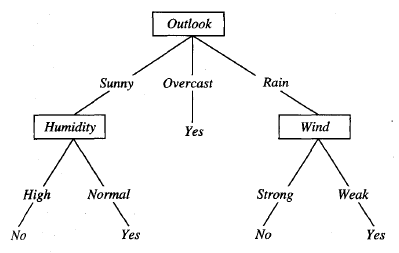
\includegraphics[scale=0.70]{img/ex_decisiontree.png}
\caption{A decision tree for the class \textit{PlayTennis} (which can take the values \textit{Yes} and \textit{No}). An example is classified by navigating through the tree to the appropriate leaf node, then returning the classification associated with this leaf. This tree classifies Saturday mornings according to whether they are suitable for playing tennis.}
\label{fig:dttennis}
\end{figure}
\end{center}

In order to select meaningful features, C4.5 measures how well a given feature separates the training examples according to their target classification. The measure it uses for this purpose is the \textit{Information Gain} measure. This measure is based on the entropy estimate, which characterizes the impurity of an arbitrary set of examples. The entropy of a sample $S$ is defined as follows:

\begin{center}$H(S) = - \sum_{i=1}^{|\mathbf{Y}|} \widehat{P}(y_i|S) \log_2 \widehat{P} (y_i|S)$\end{center}

where $\widehat{P}(y_i|S)$ is the estimated probability of examples in $S$ being labeled with class $i$. When $S$ has been partioned into $S_L$ and $S_R$ in a certain node, the weighted entropy of such a decision/split is defined as follows:

\begin{center}$H(S_L,S_R) = \frac{|S_L|}{|S|}H(S_L) + \frac{|S_R|}{|S|}H(S_R)$\end{center}

Notice entropy is 0 when all members of $X$ belong to the same class (the data is perfectly classified), and 1 if the data contains an equal proportion of positive and negative examples. Finally, the information gain for a given split then measures the expected reduction in entropy, and is defined as:

\begin{center}$Gain(S,S_L,S_R) = H(S) - H(S_L,S_R)$ \end{center}

The higher the Information Gain, the more reduction in entropy due to the split. Possible splits are evaluated and the one resulting into the highest gain is chosen. Therefore, selected trees place the features with highest information gain closest to the root. This process continues until all training examples are perfectly classified. To avoid overfitting (and to move more towards underfitting), two types of strategies can be implemented: pre-pruning and post-pruning. Pre-pruning implies that we do not allow the tree to grow completely, and stop the process in an earlier stage. Post-pruning implies that we completely grow the tree, and prune the tree afterwards.  

When the construction of a decision tree is finished, new objects can be classified. This is achieved by simply moving through the tree according to the object's feature values. The class label which is connected to the attained leaf node then represents the prediction for the class of the object.~\cite{MachineLearning97Mitchell}
 

\section{Evaluation}\label{classification-evaluation}

To decide whether to employ a   classifier we need to evaluate its classification performance. Below we consider the main  metrics for and approaches to
 classifier evaluation. 


\subsection{Evaluation Metrics}\label{eval-metrics}
Given a discrete classifier and a bag $D_t \subseteq Z$ of test instances,
we can construct a confusion matrix (see the first $|\mathbf{Y}|$ rows of the
matrix in Figure \ref{matrix:fig}). The matrix gives the counts of
the test instances depending on their true class and predicted
class provided by the classifier. We consider two types of counts:
\begin{itemize}

\item count $C_{ii}$ of true positive instances of the class $y_i \in \mathbf{Y}$ defined as instances of the class $y_i$ that
are correctly classified to belong to this class;

\item count $C_{ij}$ of false positive instances of the class $y_i \in \mathbf{Y}$ w.r.t.   the class $y_j \in \mathbf{Y}, y_i \neq y_j$ defined as instances of the class $y_j$ that are incorrectly classified to belong to the class $y_j$.
\end{itemize}

\begin{table}[h]
\centering                            % centering table
\begin{tabular}{|l| c| c c c c|}              % creating 10 columns
\hline                                % inserting double-line
& & \multicolumn{4}{|c|}{Actual} \\
\hline 
& & Class 1 & Class 2 & & Class $\mathbf{Y}$ \\ [0.5ex]
\hline                                      % inserts single-line
& Class 1 & $C_{11}$ & $C_{12}$ & \ldots & $C_{1|\mathbf{Y}|}$ \\
& Class 2  & $C_{21}$  &  $C_{22}$  & \ldots & $C_{2|\mathbf{Y}|}$ \\
\raisebox{1.5ex}{Predicted}  & & \raisebox{1.5ex}{\ldots} & \raisebox{1.5ex}{\ldots}  & & \raisebox{1.5ex}{\ldots} \\
& Class $\mathbf{Y}$ &  $C_{|\mathbf{Y}|1}$ & $C_{|\mathbf{Y}|2}$ & \ldots & $C_{|\mathbf{Y}||\mathbf{Y}|}$ \\
\hline                          % inserts single-line
\end{tabular}
\label{matrix:fig}
\end{table}

 
The counts from a confusion matrix are used for deriving useful metrics characterizing the performances of the classifier being evaluated. 

As an example, well-known metrics are accuracy rate $Ar$  and precision rate $Pr$  for class $y_i \in \mathbf{Y}$. They are
defined as follows:

\begin{eqnarray}
&&Ar = \frac{\sum_{i =1}^{|\mathbf{Y}|}C_{ii}}{\sum_{i =1}^{|\mathbf{Y}|}\sum_{k=1}^{|\mathbf{Y}|} C_{ik}} \label{a}\\
&&Pr_i = \frac{ C_{ii}}{\sum_{k=1}^{|\mathbf{Y}|} C_{ik}}  \label{p}
\end{eqnarray}

The most basic metrics are the true positive rate ({\it TPr}) of the class $y_i \in \mathbf{Y}$  and false positive rate ({\it FPr}) of the class $y_i \in \mathbf{Y}$ w.r.t. $y_j \in \mathbf{Y}, y_i \neq y_j$:


{\small
\[ TPr_i = \frac{C_{ii}}{\sum_{k=1}^{|\mathbf{Y}|} C_{ki}}\]
\[ FPr_{ij} = \frac{C_{ij}}{\sum_{k=1}^{|\mathbf{Y}|} C_{kj}}\]
}

 When the number of classes equals two, $TPr_1$ is also called sensitivity and $TPr_2$ specificity. Moreover, since the false positive rate in such case is only defined over one class, they are referred to as $FPr_1$ (the ratio of misclassifying class 1 as class 2) and $FPr_2$.

Another common metric to assess common performance over classifiers, is the area under the ROC curve. ROC curves are defined for 2-class classification problems (for simple, we call the first class the positive class, and the second class the negative class) and so-called scoring classifiers. Scoring classifiers are these classifiers that return for each instance to be classified a probability distribution. By default for 2-class problems,  if the probability of the first class is greater than 50\%, the first class is chosen. However, it is possible to choose any threshold between 0\% to 100\% to classify. Hence, we can define an infinite number of classifiers over one scoring classifier. So, a ROC curve of a scoring classifier is just the plot of the True Positive rate against the False Positive rate of all classifiers that can be achieved by changing the threshold. The idea behind this graph is that when a learner captures more instances of one class, it will generally misclassify more instances of the other class. Hence, ROC graphs depict the tradeoff between hit rates and false alarm rates of all possible classifiers. A ROC graph can be plotted by varying the probability threshold for predicting positive examples from 0 to 1. The advantage of this graph is that it shows for what region a classifier is superior compared to another. In order to come up with a single value that represents the expected performance of a ROC graph, one might measure the area under its curve, also called AUC. The AUC of a classifier is equivalent to the probability that the classifier will rank a randomly chosen positive instance higher than a randomly chosen negative instance. Thus, we should have classifiers with an AUC greater than 0.5 (which is equivalent to random guessing)~\cite{roc}~\cite{_miningwith}. 

\begin{figure}[h]
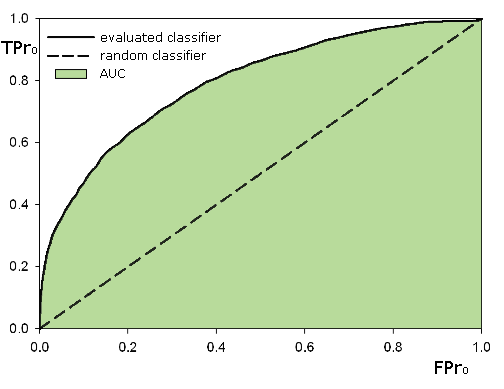
\includegraphics[scale=0.60]{img/roc-example.png}
\caption{An example of a ROC graph for class $0$ in a 2-class problem.}
\end{figure}


\subsection{Evaluation Approaches}
To evaluate classifiers we need a large independent test set. In many practical situations it is  impossible to obtain such an independent test set   since data labeling is very costly. Hence, the follwing evaluation approaches  have been proposed in order to overcome this problem. These approaches are briefly sketched below.

\paragraph{Holdout method and Random Subsampling}
In the holdout method, data is randomly partioned into two independent sets, namely a \textit{training} and a \textit{test} set. Typically, two-thirds of the data are allocated to the training set, and the remaining one-third is allocated to the test set. The training set is used to derive the model, after which the trained model is evaluated by comparing its predictions on the test set with their actual class labels. This estimate is however pessimistic, since only a portion of the initial data is used to derive the model.\\Random subsampling is a variation to the holdout method in which the holdout method is repeated \textit{k} times. The overall performance estimate is taken as the average of the performance measures obtained from each iteration.~\cite{Jiawei06}

\paragraph{Cross-validation}
In \textit{k}-fold cross-validation, the initial data are randomly partioned into \textit{k} mutually exclusive subsets (folds) each of approximately equal size. Training and testing is performed \textit{k} times. In iteration \textit{i}, fold \(D_i\) is reserved as the test set, and the remaining partitions are collectively used to train the model. Unlike the holdout and random subsampling methods, each sample is used the same number of times for training and once for testing. The overall performance is estimated by averaging the separate evaluations obtained during the \textit{k} iterations.\\Leave-one-out is a special case of \textit{k}-fold cross-validation where \textit{k} is set to the number of initial examples, such that each time only one sample is \textit{left out} at a time for the test set.

In stratified cross-validation, the folds are stratified so that the class distribution in each fold is approximately the same as that in the original dataset. In general, stratified 10-fold cross-validation is recommended for estimating classifier performance due to its relatively low bias and variance.~\cite{Jiawei06}


\subsection{Classifier Comparison}\label{classifcomp}
The metrics discussed in section~\ref{eval-metrics} allow one to compare the performance of several classifiers. However, in order to statistically prove that one classifier performs better than another, it is important that learning and evaluation is repeated several times using different training and test sets. As a result, each classifier will no longer be represented by one, but by a whole sample of values of the same performance measure. Usually, a \textit{paired t-test} is then used to compare such samples in order to calculate whether one classifier performs significantly better than another (according to the used evaluation metric). This calculation is based on the assumption that the obtained samples follow a Gaussian distribution. Thus, the paired t-test is used to compute whether the means of paired samples are equal, and therefore to prove whether one classifier produces better results than another.

\section{Conclusion}
It is clear that machine learning (ML) allows a wide variety of approaches to solve the classification task. Important to note is that no learning algorithm by definition is superior to others, but is able outperform them under specific conditions~\cite{supervised06}. Hence, the choice of any learning algorithm should be considered carefully. Preference for a certain classifier can be motivated by comparing its performance with others, as discussed in section~\ref{classification-evaluation}. However, it should be noted that restrictions regarding time or memory might hinder classifier implementation in some real-time applications.



%-------------------------------------------------------------------------------------------------------------------
% THE PROBLEM OF IMBALANCED DATASETS
%-------------------------------------------------------------------------------------------------------------------
\chapter{Classification in Imbalanced Datasets}\label{imbalanced}
Previous chapter discussed how the classification task can be solved in machine learning. However, a successful solution to this task can be seriously hindered. For example, complications can arise when when we have class imbalanced data: a class of interest is heavily under-represented in comparison to other classes. This problem and its implications are described in section~\ref{imbalanced-theproblem} and~\ref{causestheproblem}. Although no global solution has yet been found, many approaches have been introduced during the past decade. We discuss some of these approaches in section~\ref{approaches}. Finally, we finish in section~\ref{imb-summary} with a conclusion.


\section{Problem Description}\label{imbalanced-theproblem}
An imbalanced (or skewed) dataset occurs when a class of interest is heavily under-represented in comparison to the other classes.  These kind of datasets occur in many applications, such as medical diagnosis/monitoring, fraud/intrusion detection, text categorization, risk management, information retrieval and filtering tasks.  Moreover, when the data collection process is limited or very time consuming, it might happen that class imbalances occur in domains that do not have an intrinsic imbalance.  Typical, the ratio of the small to the large class takes proportions such as 1 to 100, 1 to 1\,000, 1 to 10\,000 or even more. Since many standard classifiers try to maximize accuracy and do not alter the distribution from the training data, they tend to be overwhelmed by the large classes and ignore the small ones~\cite{ProvostMLID}. The reason why should be clear: predicting the majority class in imbalanced datasets will easily yield accuracies of more than 99\%. 

%-------------------------------------------------------------------------------------------------------------------
% Implications of Class Imbalance
%-------------------------------------------------------------------------------------------------------------------
\section{Class Imbalance, Noise, and Outliers}\label{causestheproblem}
Class imbalance is mainly related to rarity, of which two different situations can occur. The first type of rarity is called \textit{rare classes}, and concerns the poor presence of instances of a specific class. The second type of rarity concerns \textit{rare cases}, which correspond to a meaningful but relatively distant cases of the classes. For simplicity, we call this rare cases \textit{outliers}. Although rare classes and outliers are not directly related, empirical studies show that the minority class contains a greater proportion of outliers than the majority class~\cite{Weiss03learningwhen}. Since in many situations outliers cannot be distinguished from class noise, recognizing more (less) outliers more likely results into overfitting (underfitting) the minority class. Besides class noise, the existence of feature noise can significantly influence the distribution of the minority data. When feature noise occurs in minority class clusters, affected instances can become outliers. On the other hand, when feature noise occurs in outliers, affected instances can disappear within the minority class clusters. Hence, recognizing more (less) outliers may again result into overfitting (underfitting). When the minority data is scattered, feature noise does not have this effect.~\cite{Japkowicz02classimbalance}~\cite{Prati04classimbalances}~\cite{miningwith04}


%-------------------------------------------------------------------------------------------------------------------
% CURRENT SOLUTIONS
%-------------------------------------------------------------------------------------------------------------------
\section{Approaches}\label{approaches}
In order to overcome the class imbalance problem, many approaches have been introduced. The most famous approaches try to tackle the lack of the minority data by increasing their number through sampling (section~\ref{sampling-techniques}) or cost-sensitivity (section~\ref{cost-sensitivity}). Other approaches try to identify the minority objects, rather than the separation between the minority and the majority data (section~\ref{one-class}). Classifier improvements can also be obtained by altering the feature selection process in learning algorithms such as CART or C4.5. Often, measures used in this process are based on unreliable estimates or favor the recognition of the majority class. We discuss some improvements for these measures and estimates in section~\ref{feat-select}. More improvements can be obtained by using different evaluation metrics, as many of them do not value rarity well. However more appropriate metrics have already been discussed, we give a short summary in section~\ref{app-eval-metric}. A last approach considers combining a set of classifiers (also called a classifier ensemble), with the goal to obtain more reliable predictions than a single classifier (section~\ref{classif-ensembles}). 



\subsection{Sampling techniques}\label{sampling-techniques} 
Sampling is probably the most-direct approach to handle class imbalances. It changes the priors in the training set by either increasing instances from the minority class (\textit{over-sampling}), decreasing instances from the majority class (\textit{under-sampling}), or a combination of both. As a result, the class distribution of the training data is changed such that the resulting data is more balanced. Although general implementation is fairly simple, some disadvantages threaten its use.  First of all, under-sampling might discard useful data, what would lead to under-fitting the (majority class) data. On the other hand, over-sampling might result into overfitting the (minority class) data, since most over-sampling methods generate exact copies of existing instances. Moreover, over-sampling increases the size of the training set, which will increase the time necessary to learn the classifier~\cite{mccarthy}.

Sampling techniques are a direct approach to tackle with class imbalances, and can be used in combination with any classifier. Moreover, under-sampling allows a solution to the enormous data sets which size needs to be reduced.  Finally, the use of sampling rates allows the fine-tuning of class imbalances, and therefore their resulting classification models and performance.  

\subsubsection{Monte Carlo Sampling}
Monte Carlo methods were introduced in 1949 by Metropolis and Ulam~\cite{Metropolis49MonteCarlo}, and are a class of computational algorithms that rely on repeated random sampling in order to perform a specific task. In the context of over-sampling, the goal is to generate samples from the minority distribution. This can for example be achieved by sampling with replacement from the minority distribution, a technique known as bootstrapping. In the same way, bootstrapping can be used to under-sample the majority distribution.

An important example of Monte Carlo sampling is the Gibbs sampling algorithm. Gibbs sampling generates a sequence of samples from the joint probability distribution of two or more random variables. The purpose is to approximate the joint distribution, or to compute an integral (such as expected value).  Gibbs sampling was introduced by Stuart German \& Donald German~\cite{Stochastic84} in the context of image processing and then discussed in the context of missing data problems by Tanner \& Wong~\cite{calcpost87}. Gibbs sampling is applicable when the joint distribution is not known explicitly, but the conditional distribution of each variable is known.  The Gibbs sampling algorithm generates an instance from the distribution of each variable in turn, conditional on the current values of the other variables.  It can be shown that the sequence of samples constitutes a Markov chain, and the stationary distribution of that Markov chain is just the sought-after joint distribution. 

Other extensions which are related to Monte Carlo methods are Rejection sampling, Importance sampling, Gibbs sampling and Slice sampling~\cite{bishop}~\cite{Neal03slicesampling}.

\subsubsection{SMOTE}\label{smote}
\index{sampling techniques!SMOTE}
Synthetic minority over-sampling technique (SMOTE) was introduced by Cieslak \& Chawla, who suggest a local implementation of sampling based on the belief of multi-modality of many datasets~\cite{StartGlobally08}~\cite{smote}.  Instead of over-sampling with replacement, SMOTE creates "synthetic" instances along the line segments joining any/all of the \textit{k} minority class nearest neighbors. Hence, SMOTE is a generative sampling model. Since generated instances are strongly related to existing instances, this approach forces the decision region of the minority class to become more general (avoid overfitting).  When combined with under-sampling, SMOTE tends to improve overall performance compared to over-sampling with replacement.  Although implementation increases computational cost of the learning algorithm, experiments have shown the convenience of applying SMOTE when the data set has very few positive (minority) instances~\cite{batista}.



\subsection{Cost-sensitive Learning}\label{cost-sensitivity}
\index{costsensitive learning}
Another approach to deal with imbalanced datasets, is to introduce cost-sensitivity during the training or evaluation of a classifier. This allows the classifiers to focus more on predicting specific classes, and can be achieved by assigning costs to each type of (mis)classification. Usually, these costs are accepted as user input and learned by comparing various cost settings. The set of assigned costs for a classifier is often given by a \textit{cost matrix}, and looks as follows:

\begin{table}[h]
\centering                            % centering table
\begin{tabular}{|l| c| c c c c|}              % creating 10 columns
\hline                                % inserting double-line
& & \multicolumn{4}{|c|}{Actual} \\
\hline 
& & Class 1 & Class 2 & & Class $\mathbf{Y}$\\ [0.5ex]
\hline                                      % inserts single-line
& Class 1 & $CM_{11}$ & $CM_{12}$ & \ldots & $CM_{1|\mathbf{Y}|}$ \\
& Class 2  & $CM_{21}$  &  $CM_{22}$  & \ldots & $CM_{2|\mathbf{Y}|}$ \\
\raisebox{1.5ex}{Predicted}  & & \raisebox{1.5ex}{\ldots} & \raisebox{1.5ex}{\ldots}  & & \raisebox{1.5ex}{\ldots} \\
& Class $\mathbf{Y}$ &  $CM_{|\mathbf{Y}|1}$ & $CM_{|\mathbf{Y}|2}$ & \ldots & $CM_{|\mathbf{Y}||\mathbf{Y}|}$ \\
\hline                          % inserts single-line
\end{tabular}
\label{tab:PPer}
\end{table}

Summarized, a cost matrix describes the cost of classifying an object of class $i$ (actual class) as class $j$ (predicted class) in entry $CM_{ij}$. Since misclassifying is costly, usually $CM_{ij} \geq 0$ if $i \neq j$, and, since correct classification does not cost anything, $CM_{ij}  = 0$ if \(i = j\). However, some classifiers induce a gain (negative cost) $CM_{ij} \leq 0$ for correctly classifying instances in order to quantify the consequences of a good classification.

In a 2-class classification problem (where the second class describes the minority data), the cost assignments are usually the following:
\begin{itemize}
\item $CM_{11} = CM_{22} = 0$
\item $CM_{21} = 1$
\item $CM_{12} > 1$
\end{itemize}

Cost-sensitive learning employs the cost-sensitive matrix. There are different scenarios given below:

\begin{itemize}
\item \textbf{Clasifier evaluation}: an easy solution to implement costs is to apply them in the classifier evaluation. An \textit{expected misclassification cost} can be calculated by making a cross-product between the misclassification cost matrix and the confusion matrix, which allows comparison of models.
\item \textbf{Minimizing expected cost}: in this approach, the costs are handled during the learning process. The classifier is trained without considering the costs, but uses a classification rule that minimizes the expected loss. Conditional probabilities provided by the model are used to calculate the loss associated with each decision, and the decision which minimizes the expected loss is then chosen. The main advantage of this approach is that it allows to use, without specific modifications, the results provided by the classifier output.
\item \textbf{Instance reweighting}: this approach will assign a weight to each training instance according to its misclassification cost, and can therefore be compared to sampling techniques, with the difference that the number of instances does not change.
\item \textbf{Class probability thresholds}: some classifiers, such as the Naive Bayes classifier or some Neural Networks, yield a score that represents the degree to which an instance is a member of a class.  In such cases, altering the threshold which decides whether the instance is labeled as positive or negative, can produce several classifiers. For example, classifiers generally use 0.50 as threshold value, meaning that if the classifier output for a specific instance is above 50\%, the classifier produces a \textbf{Y}, else a \textbf{N}.  If this threshold value is now altered to 0.60, a different classifier will be obtained.  This technique is used in the construction of ROC graphs~\cite{roc}.
\end{itemize}
Results of a comparative study~\cite{mccarthy} show that cost-sensitive learning and over-sampling perform similarly whereas under-sampling performs much worse.  When datasets are very large, cost-sensitive learning seems to outperform other techniques, perhaps because the larger amount of training data makes it easier to estimate more accurately the class-membership probabilities.  However, although cost-sensitivity allows a flexible solution to class imbalances, recent studies have shown that clever re-sampling and combination methods can do more than cost-sensitive learning as they provide new information or eliminate redundant information for the learning algorithm.~\cite{Chawla04editorial:special}


\subsection{One-Class Learning}\label{one-class}
One-class learning is a different approach which proves particularly useful on extremely imbalanced data sets with a high-dimensional noisy feature space~\cite{raskutti}. As recognition-based approach, it learns a classifier which can predict samples of one (usually the minority) class.  Therefore, this approach differs from sampling and cost-sensitivity since it does not consider the class imbalance as a problem. It focuses on the separation between the minority and the majority classes.

There are two main strategies for one-class learning. The first one tries to recognize instances of the (usually) minority class rather than discriminate between instances of all classes. As a result, the goal of this strategy is to define a boundary around the target class such that as many objects as possible of the target classes are recognized, while a minimal amount of outliers are accepted. 
The second approach to one-class learning uses instances of both classes to make predictions about the target class, and uses internal bias strategies during the learning process to achieve this goal~\cite{one-class-classification}~\cite{REMED}.

An example of the first approach to one-class learning is Rule Extraction for MEdical Diagnosis (REMED)~\cite{REMED}. This approach is designed to deal with the imbalanced class problem, and to provide predictions with a reliability measure. REMED is a symbolic one-class approach to solve binary classification tasks. It is trained with instances of both classes and implements internal strategies during the learning process to maximize the correct prediction of the minority class instances. In general, REMED generates rule systems which are supported by attribute selection based on simple logistic regression to test the association and its confidence (99\% or 99.99\%) with the studied disease.

An example of the second approach to one-class learning can be found in so-called \textit{separate-and-conquer rule learning} or \textit{covering algorithms}~\ref{sepandconq}. These algorithms basically search for a rule that explains a part of the training instances, separate them and recursively conquer the remaining instances by learning more rules until no instances remain. As a result, they do not necessarily focus on one class. Since this technique can easily lead into overfitting, constraints are often relaxed by the use of stopping criteria and/or post-processing methods~\cite{sepandconq}. A typical covering algorithm is RIPPER, which generates rules for each class from the minority class to the majority class~\cite{jrip}~\cite{Kotsiantis06}.


\subsection{Feature Selection}\label{feat-select}
Many learning algorithms such as decision tree learning employ feature selection in order to build a classifier (see section~\ref{classifier-example}). The main idea of feature selection is to choose a subset of input features by eliminating features with little or no predictive information according to some measure. As a result, feature selection has a significant influence on the inductive bias of the classifiers. To adopt feature selection within the imbalanced problem, there exist two approaches. The first one is based on adapting class-probability estimates. The second approach is based on the introduction of new feature selection measures. 

To adapt feature selection measures (such as Information Gain), we can modify the way we estimate the class-probabilities. For example, if there are \(N_i\) instances of a class \(i\) at a leaf and \(|\mathbf{Y}|\) classes, then the probability that an instance at the leaf is a member of class \(i\) is given by:

\begin{eqnarray}
&&\hat{P}(y_i|x) = \frac{N_i}{\sum_{j=1}^{|\mathbf{Y}|}{N_j}}
\end{eqnarray}

When data is sparse, this estimate can be very unreliable. For this reason, several smoothing techniques have been introduced to improve the quality of the estimates. 

The Laplace estimate smooths the probability estimates by introducing a prior probability \(1/|\mathbf{Y}|\)~\cite{probest06}:

\begin{eqnarray}
&&\hat{P}(y_i|x) = \frac{N_{i}+1}{|\mathbf{Y}| + \sum_{j=1}^{|\mathbf{Y}|}{N_j}}
\end{eqnarray}

However, Laplace estimates might not be very appropriate for highly imbalanced datasets (Zadrozny \& Elkan 2001).  In those cases, it could be useful to incorporate the prior of positive class to smooth the probabilities so that the estimates are shifted towards the minority class base rate.  

A more general estimate than the Laplace estimate, is the so-called m-estimate. This estimate uses a parameter \(m\) which controls the role of the prior probabilities \(b_i\) of the considered class \(i\) and the evidence provided by the instances.

\begin{eqnarray}
&&\widehat{P}(y_i|x) = \frac{N_{i}+mb_i}{m + \sum_{j=1}^{|\mathbf{Y}|}{N_j}}
\end{eqnarray}

Higher values for \(m\) give more weight to the prior probabilities and less to the instances, therefore appropriate for datasets that contain more noise. The prior \(b_i\) can be estimated from the training set using relative frequency. We note that the Laplace estimate is a special case obtained by setting \(m\) to \(|\mathbf{Y}|\), and \(b\) to \(1/|\mathbf{Y}|\) for all classes (uniform distribution).

Another approach to improve the quality of the estimates was introduced by Nitesh \& Chawla~\cite{probest06}. They propose an ensemble method to smooth out the probability estimates at the leaves by bagging decision trees. The different estimates for $\hat{P}(y_i|x)$ are averaged, therefore improving the quality of the estimates and reducing the variance.\\

In stead of improving the probability estimates, one can also try to improve the actual measure used for feature selection. A typical measure used in decision tree learning is Information Gain, which uses entropy to characterize the impurity of an arbitrary set of instances. The problem with this (and many other) measure is that it associates most of the features in imbalanced datasets with the majority class~\cite{Zheng04featureselection}.

In order to overcome this problem, Cieslak \& Chawla proposed a variant of Hellinger distance (which is a measure of distributional divergence) as a new measure for feature selection. This measure mainly captures the divergence between feature values given two or more different classes. Since the prior does not influence the distance calculation, Hellinger distance is a skew insensitive measure.~\cite{hellinger}. 

Assuming a two-class problem, its calculation is based on the class-within presence of positive and negative instances compared to their overall presence.  Since Hellinger distance does not take the distribution over the classes into consideration, it favours the recognition of minority classes.

\begin{figure}[h]
\centering
\subfloat[10000:10000]{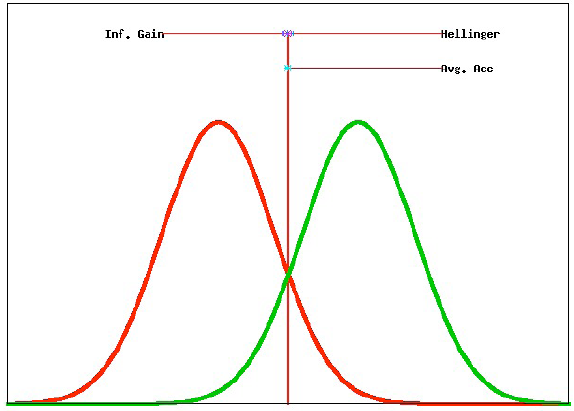
\includegraphics[scale=0.35]{img/Hellinger_01.png}}                
\subfloat[1000:10000]{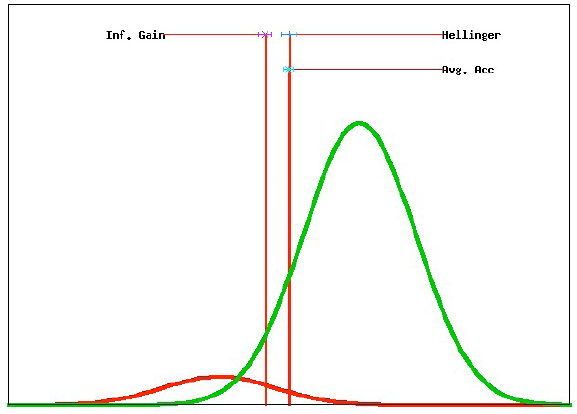
\includegraphics[scale=0.35]{img/Hellinger_02.png}}  
\caption{The effect of class imbalance (figure b) on the measures Information Gain and Hellinger distance.}
\end{figure}

In a two-class problem, let \(S_1\) be a sample of class 1 and \(S_2\) be a sample of class 2. Assuming the sample \(S\) is distributed over \textit{p} partitions in a certain feature, the Hellinger distance between \(S_1\) and \(S_2\) within that feature is defined as follows:

\begin{eqnarray}
&&Hellinger \left (S,S_1,S_2 \right)=\sqrt{\sum_{j=1}^p {\left(\sqrt{\frac{|\mathbf{S}_{1j}|}{|\mathbf{S}_1|}} - \sqrt{\frac{|\mathbf{S}_{2j}|}{|\mathbf{S}_2|}} \right )^2}}
\end{eqnarray}

where \(S_k\) stands for the number of instances of class \(k\) and \(S_{kj}\) for the number of instances of class \(k\) having feature value \(j\) for the considered feature.

The problem with Hellinger distance however is that techniques such as sampling will have a negative effect on its implementation~\cite{mccarthy}, which harms the goal to create a classifier that performs well across a range of cost/priors~\cite{Chawla04editorial:special}.  This means that the splitting dilemma is simplified to an almost unconfigurable implementation where classification is only based on relative proportions of the data and the use of (some) metaclassifiers has become obsolete.

\subsection{Alternative Evaluation Metrics}\label{app-eval-metric}
As discussed earlier, evaluation metrics are used to value the performance of a classifier. Often, accuracy is used for this purpose. The problem however with metrics such as accuracy is that they do not adequately value rarity. Since one would like to know how well a classifier performs on the minority (positive class) data as well, using more appropriate metrics is important. The True Positive rate and False Positive rate prove excellent for this purpose, as they measure performance on the minority class separately. Well-known metrics based on these rates are without doubt the AUC and sensitivity/specificity. The benefit of ROC curves is that they allow to explore tradeoff among different classifiers for different misclassification cost and class distributions. The area under the ROC curve (AUC) can then be used to compare the expected class-probability tradeoff (and therefore also the obtained class separation) of different classifiers. 


\subsection{Classifier ensembles}\label{classif-ensembles}
The main idea of classifier ensembles is to learn a set of classifiers in stead of a single one, and to combine their predicitions when classifying new objects. Hence, predictions are less dependent on peculiarities of a single training set, and the combination of multiple classifiers may learn a more expressive concept~\cite{DietterichEnsemble02}. As a result, classifiers ensembles often reduce the bias and/or variance in the classification process.  These properties make ensembles an interesting approach to imbalanced datasets. Many studies which use ensembles to overcome class imbalances, combine the results of several classifiers, each induced after over-sampling or under-sampling the data with different rates~\cite{garcia}. Although there exists a wide variety of ensemble techniques, many approaches to imbalanced datasets are based on bagging or random forests.

\textbf{Bagging}, also called \textit{bootstrap aggregation}, is based on constructing different specialized classifiers. It does so by providing each classifier with a different training bag, which is sampled uniformly and with replacement from the original training set. Usually, minority training instances are sampled with a different ratio than majority instances, such that over-/under- sampling is performed in each training set~\cite{1137548}~\cite{Breiman96b}~\cite{confsdmHidoK08}. This allows each classifier to focus more (specialize) on specific aspects of the minority data. After a set of different classifiers is trained, their predictions are combined by voting. As a result, the ensemble will have a better grasp of the relevant concepts than a single classifier, since mistakes made by each classifier are neglected by the voting scheme. Bagging proves especifically successful when applied to classifier learning methods that are sensitive (instable) to modifications of the input data~\cite{Breiman94Heur}.

Another classifier ensemble related to bagging considers the construction of \textbf{random forests}~\cite{Breiman01randomforests}. These forests are a combination of tree predictors, each trained on a bootstrapped sample (similar to bagging). Again, these samples can be obtained by over-sampling the minority data or under-sampling the majority data~\cite{Chen04RF}. Finally, predictions are combined by voting. The difference with bagging is that random forests also implement random effects within the classifiers (eg by the use of random feature selection). Hence, random forests increase the level of randomization steering the classification process. The advantage is they can cope with small datasets containing a large amount of features that can describe complex interactions and even be highly correlated~\cite{strobl08why}. As these problems typically occur in imbalanced datasets, random forests are an interesting approach in such situations.

As discussed in~\ref{feat-select}, bagging can also be implemented to obtain a better estimate of class probabilities. An example of this approach is MetaCost, which uses bagging to improve these estimates in cost-sensitive learning, another typical approach to imbalanced datasets~\cite{domingos99MetaCost}. Here, costs are introduced by applying the Bayes optimal prediction, such that for a prediction for \textit{x} the class \textit{j} minimizes the conditional risk: \(R(y_i|x) = \sum_{j}\widehat{P}(y_j|x)\,CM_{ij}\). MetaCost estimates these class probabilities by learning multiple classifiers and voting over the predictions, therefore a variant to Breiman's \textit{bagging} technique. The difference with bagging is in the number \textit{r} of instances in each resample may be smaller than the training size \textit{n}.

\section{Conclusion}\label{imb-summary}
In this chapter we showed that the class imbalance problem imposes a practical challenge for the classification task. If no special techniques are used  the classifiers that are used have to find a correct balance between being overfitted and underfitted (see section~\ref{causestheproblem}). We showed that there exist plenty of techniques for the class imbalance problem. Among them it is worth mentioning sampling techniques like bagging (based on the minority class) and generative techniques like SMOTE. In the next section we propose considering a combination of these two techniques. In addition, we would like to stress the importance of class-related metrics for classfier evaluation in the presence of  class imbalance. Hence, in the rest of the thesis we use sensitivity, specificity, and AUC.


\chapter{Novel approach to Classification in Imbalanced Datasets}\label{newapproach}
In previous chapter, we discussed approaches that improve classification for imbalanced datasets. We concluded that sampling and bagging techniques represent interesting approaches, as they can be applied to any classifier without the need to change them. Although especially synthetic samplers are promising (since they help to avoid overfitting), their implementation in imbalanced datasets is difficult. This is because the lack of data forces them to make some assumptions. As a result, these samplers will have worse performance when the posed assumptions do not hold or interfere with assumptions of the classifiers. We discuss this problem in section~\ref{rnd-intro}. In order to avoid this problem, we propose a new approach for classification in section~\ref{rnb-approach} that takes the assumptions of sampler and classifier into account. For this reason, a new sampler is introduced and explained in section~\ref{rnb-implementation}. Afterwards, this sampler is used in a specific setup such that all the posed assumptions are met and validated. We discuss the implications of this setup in section~\ref{rnb-implication} and show how the proposed approach allows reducing the variance in some situations. Finally, we formulate a conclusion in section~\ref{rnb-conclusion}.


\section{Introduction}\label{rnd-intro}
In the previous chapter we discussed how several techniques allow to improve the recognition rate of the minority class in imbalanced datasets. We also discussed that elegant solutions are mainly to be found in the use of ensembles and sampling techniques, since they do not require alterations in the base classifier. Experiment results in chapter~\ref{Experiments} show that these techniques indeed improve classifier performance. However, the results also show that one particular (synthetic) sampler, namely SMOTE, yields a performance degrade in many classifiers. The idea behind this observation is that when posed assumptions do not hold or interfere with the ones of the applied classifier, synthetic samplers such as SMOTE performs worse. For example, SMOTE assumes that the minority data are forming clusters of at least \(k\) instances. It then generates synthetic samples based on the existing within-cluster variance. When these assumptions do not hold, SMOTE will increase (rather than decrease) the existing level of noise. Moreover, experiments in chapter~\ref{Experiments} show that SMOTE significantly reduces the performance in a Naive Bayes classifier. This is probably related to the fact that SMOTE does not maintain the separate feature distributions.  Hence, we can conclude that the introduction of synthetic samplers in imbalanced datasets is a risky strategy. Another danger regarding synthetic samplers is that they often rely on feature interactions in order to approximate the minority distribution. Since the minority class data size is small, many of the captured feature interactions are very unreliable. Moreover, when the amount of features is large, most of these interactions are not even present in the training data. Hence, it is reasonable to mistrust the occurring feature interactions, and to impose feature independency in the minority dataset. The result is that by applying this technique, we can obtain samples that perfectly match the assumptions of a Naive Bayes classifier. In the next section, we discuss the approach of this technique.


\section{Approach}\label{rnb-approach}
In order to impose feature independency in the minority samples, we propose the following (synthetic) sampling scheme. Over-sample the minority distribution by creating (synthetic) instances where the feature values are bootstrapped independently from their original minority feature distribution. We call this sampler the \textbf{Naive Bayes Sampler} (NBS). We can say that NBS generates synthetic instances by randomly selecting (with replacement) feature values from their resp (minority class) prior distributions. The effect of NBS is illustrated in figure~\ref{fig:NBS}. Since NBS generates samples that are feature independent, they can best be used to train a Naive Bayes classifier (which assumes maximum conditional independence). Moreover, since the generated samples are influenced by a randomization process, the use of a bagging ensemble is favoured in order to decrease the variance over the estimates. Hence, we can summarize the proposed approach as follows:


\begin{enumerate}
\item \textbf{Over-sampling}: Create \textit{K} new (training) samples by copying the majority data, and creating \(o \times n_{minority}\) synthetic minority examples by bootstrapping from the individual feature values in the original minority dataset. The parameter \(o\) is defined by forehand and describes the oversample ratio.
\item \textbf{Bagging}: Train a Naive Bayes classifier on each separate generated training sample. These \textit{K} classifiers are then used to form a bagging ensemble.
\item \textbf{Prediction}: Test data is predicted by averaging the votes of the individual classifiers in the classifier ensemble.
\end{enumerate}

Since the disscussed approach introduces randomization in a Naive Bayes classifier by bootstrapping over feature-values, we call this approach \textbf{Random Naive Bayes by Feature-value Bootstrapping} (RNB-FvB). The experiment results of this approach can be found in section~\ref{exp-rnb}.







%-------------------------------------------------------------------------------------------------------------------
% IMPLEMENTATION
%-------------------------------------------------------------------------------------------------------------------
\section{Implementation}\label{rnb-implementation}
The following paragraphs explain in detail how this bootstrapping can be applied to nominal and numeric features.

Boostrapping nominal feature values is achieved by assigning feature values to synthetic instances by bootstrapping from their prior distribution. With other words, if \(N\) instances in training bag $B$ belong to class \(i\) and have feature value $v$ (out of $p$ possible feature values) for a given feature, the probability of selecting that feature value for an artificial object of class $i$ equals:

\begin{eqnarray}
&& P(v_i|B)=\frac{N_{iv}}{\sum_{j=1}^p{N_{ij}}}
\end{eqnarray}

Note that we also consider \textit{missing values} as a possible feature value.

\begin{figure}[h]
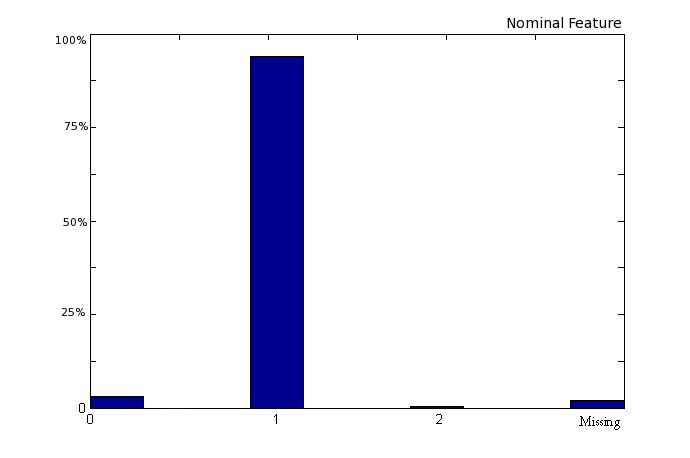
\includegraphics[scale=0.65]{img/nominalEst.png}
\caption{Bootstrapping nominal features}
\end{figure}

Bootstrapping numeric feature values is applied by a slightly more advanced technique. First, mean and variance of the prior distribution are estimated using Maximum Likelihood Estimation. These parameters are then used to generate new feature values along the prior (Gaussian) distribution. In order to avoid invalid feature values (for example when numeric features can only take positive values), their range of validity is defined. When an invalid feature value is then selected, it is assigned a new feature value according to the uniform distribution over the defined range. Hence, the original Gaussian distribution is augmented by a uniform distribution and only exists over the defined range.

\begin{landscape}
\begin{figure}[h]
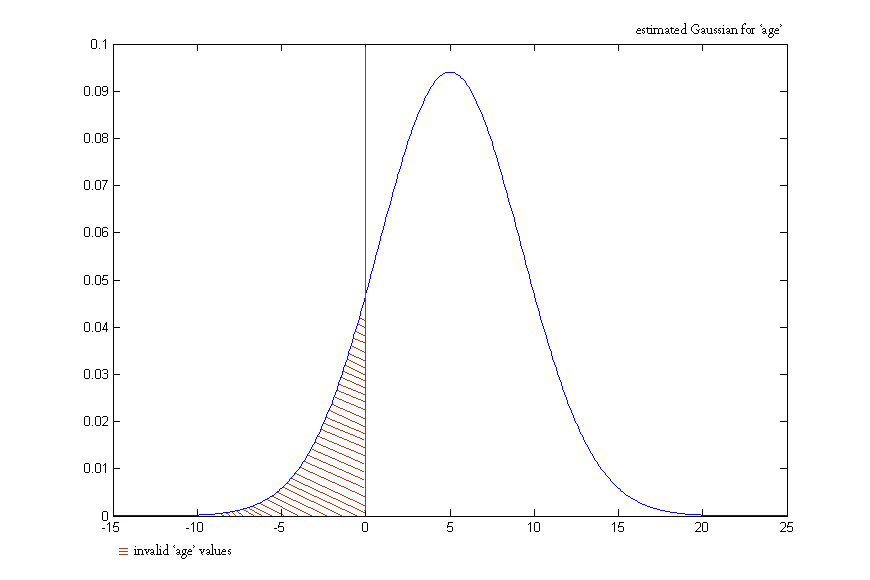
\includegraphics[scale=0.55]{img/AgeRegress.png} 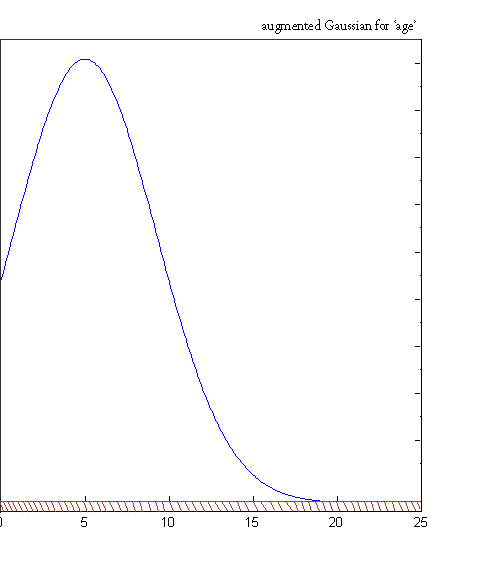
\includegraphics[scale=0.55]{img/AgeRegress2.png} 
\caption{Bootstrapping numeric feature values}
\end{figure}
\end{landscape}




%-------------------------------------------------------------------------------------------------------------------
% IMPLICATIONS
%-------------------------------------------------------------------------------------------------------------------
\section{Implications}\label{rnb-implication}
As a logical result of NBS, obtained samples will follow a different distribution than the ones obtained by (regular) bootstrapping. This idea is illustrated in figure~\ref{fig:NBS}, and in the following example. Assume a minority dataset $Z$ which is described by a binary class $Y$ and two binary features ($X_1$ and $X_2$), such that $Z = X_1 \times X_2 \times Y$:

\begin{table}[h]
\centering  
\begin{tabular}{ c c c}    
Feature 1 & Feature 2 & Class Label\\
\hline
1& 1& 1\\
1& 0& 1\\
0& 1& 0\\
0& 0& 1\\
1& 1& 1\\
1& 0& 0\\
0& 0& 0\\
1& 0& 0\\
\end{tabular}
\label{tab:exampleZ}
\caption{A possible minority dataset $Z$} % title name of the table
\end{table}

If we consider the sampling schemes (1) NBS and (2) bootstrapping, we can say the following:

\begin{itemize}
\item In (1), feature values are bootstrapped independently from $X_1$ and $X_2$ such that $P(X_1)$ and $P(X_2)$ become independent in the samples:
\begin{eqnarray}
P(X_1 \wedge X_2) &=& P(X_1 \cap X_2) \nonumber \\
&=& P(X_1|X_2)\;P(X_2) \nonumber \\
&=& P(X_1)\;P(X_2) \label{eq:px1px2indep}
\end{eqnarray}
\item In (2), instances are bootstrapped from $Z$ such that $P(X_1 \wedge X_2)$ is more or less preserved in the samples. This also means that feature dependencies are remained in the samples, such that:
\begin{eqnarray}
P(X_1 \wedge X_2) &=& P(X_1 \cap X_2) \nonumber \\
&=& P(X_1|X_2)\;P(X_2) \label{eq:px1px2dep} \\
&\neq& P(X_1)\;P(X_2) \nonumber
\end{eqnarray}
\end{itemize}

If we repeat the sampling process multiple times by creating a bagging ensemble, the distributions of $P(X_1)$ and $P(X_2)$ behave as random variables. In (1), these disributions will be independent, while in (2) these distributions will be correlated. Although a Naive Bayes classifier does not consider the feature dependencies present in the training data, we explain how existing correlations influence the variance of the estimates in a Naive Bayes classifier. The decision boundary for $Y$ in Naive Bayes is given as:

\begin{eqnarray}
Y &\longleftarrow& \mbox{arg max $y$ }\;\frac{\hat{P}(Y = y) \prod_{i=1}^m{\hat{P}(X_i|Y=y)}}{\sum_{j=1}^{|Y|}{\hat{P}(Y=y_j)} \prod_{i=1}^{m}{\hat{P}(X_i|Y=y)}} \label{eq:naivebayesdenom}\\
&\longleftarrow& \mbox{arg max $y$ }\;\hat{P}(Y = y) \prod_{i=1}^m{\hat{P}(X_i|Y=y)}\label{eq:naivebayesnodenom}
\end{eqnarray}

Equation~\ref{eq:naivebayesnodenom} allows us to calculate the variance over the estimates of $Y$ when we construct a bagging ensemble of Naive Bayes classifiers using sampling schemes (1) and (2). Please note that the expression $\sum_{j=1}^{|Y|}{\hat{P}(Y=y_j)} \prod_{i=1}^{m}{\hat{P}(X_i|Y=y)}$ differs in sampling scheme (1) and (2), as the estimates come from a different distribution.  However, for sake of simplicity we assume that this difference can be neglected \footnote{In figure~\ref{fig:varab} and \ref{fig:varabss100}, we can see that this simplification does not alter the type of relationship between the covariance of the prior probabilities and $\mbox{Var}\big(\hat{P}(Y=y|x)\big)$.} and continue from equation~\ref{eq:naivebayesnodenom}:

\begin{eqnarray}
\mbox{Var}\big(\hat{P}(Y=y|x)\big) &\propto& Var \big (\hat{P}(Y = y) \prod_{i=1}^m{\hat{P}(X_i|Y=y)} \big )\label{eq:varNBfull}
\end{eqnarray}

Since both in (1) and (2) we have that $P(Y = y)$ is a constant that represents the likelihood of the class $y$, we can rewrite equation~\ref{eq:varNBfull} as follows:

\begin{eqnarray}
\mbox{Var}\big(\hat{P}(Y=y|x)\big) &\propto& \mbox{Var} \big (\prod_{i=1}^m{\hat{P}(X_i|Y=y)} \big )
\end{eqnarray}

If we consider a dataset which is described by two features $X_1$ and $X_2$, we can rewrite previous equation as:

\begin{eqnarray}
\mbox{Var}\big(\hat{P}(Y=y|x)\big)) &\propto& \mbox{Var} \big (\hat{P}(X_1|Y=y)\, \hat{P}(X_2|Y=y)\big )\label{eq:nbsimplified}
\end{eqnarray}

Since $\hat{P}(X_1|Y=y)$ and $\hat{P}(X_2|Y=y)$ are random variables, we need to know how we can work out the variance of their product. As expressed by Goodman~\cite{exactvar60}, the variance of a product of two random variables $a$ and $b$ is equal to:

\begin{eqnarray}
\mbox{Var}(ab) &=& A^2\,\mbox{Var}(b) + B^2\,\mbox{Var}(a) + 2ABE_{11} \nonumber \\
&& + 2AE_{12} + 2BE_{21} + E_{22} - E_{11}^2\label{eq:varxy}\\
&\approx& A^2\,\mbox{Var}(b) + B^2\,\mbox{Var}(a) + 2ABE_{11}\label{eq:varxyapprox}
\end{eqnarray}

where 

\begin{itemize}
\item $A = E(a)$ : the expected value of $a$
\item $B = E(b)$ : the expected value of $b$
\item $E_{ij} = E\ \big ((a-A)^i (b-B)^j\big )$
\end{itemize}

Often, Var($ab$) is approximated by equation~\ref{eq:varxyapprox}. Since by definition $\mbox{Cov}(a,b) = E \big ( (a-E(a))(b-E(b) \big )$, we can say that $E_{11}$ is the covariance between $a$ and $b$. When feature independence holds, we can say the following:

\begin{eqnarray}
E(ab) &=& E(a)\;E(b)
\end{eqnarray}

and therefore:
\begin{eqnarray}
E \big ( (a + Ct_1) (b + Ct_2) \big ) &=& E (a + Ct_1)\; E(b + Ct_2)
\end{eqnarray}

This means that when feature independence holds, we can simplify equation~\ref{eq:varxy} as follows:

\begin{eqnarray}
\mbox{Var}^I(ab) &=& A^2\,\mbox{Var}(b) + B^2\,\mbox{Var}(a) + 2ABE_{11} + 2AE_{12} + 2BE_{21} + E_{22} - E_{11}^2 \nonumber \\
&=& A^2\,\mbox{Var}(b) + B^2\,\mbox{Var}(a) + 2ABE \big ((a-A) (b-B) \big) \nonumber \\
&& + 2AE \big ((a-A) (b-B)^2 \big ) + 2BE \big ((a-A)^2 (b-B) \big ) \nonumber \\
&& + E \big ((a-A)^2 (b-B)^2 \big ) - E^2 \big ((a-A) (b-B) \big )\nonumber \\
&=& A^2\,\mbox{Var}(b) + B^2\,\mbox{Var}(a) + 2ABE (a-A) \,E (b-B) \nonumber \\
&& + 2AE (a-A) \,E \big ( (b-B)^2 \big ) + 2BE \big ((a-A)^2 \big ) \,E(b-B) \nonumber \\
&& + E \big ((a-A)^2 \big ) \, E \big ((b-B)^2 \big ) - E(a-A)E(a-A)\,E(b-B)E(b-B) \nonumber \\
\nonumber \\
&& \mbox{where $E(a-A) = E(a)-E(A) = E(a) - E(E(a)) = E(a) - E(a) = 0$} \nonumber\\
&& \mbox{and similartly $E(b-B) = 0$} \nonumber\\
\nonumber \\
&=& A^2\,\mbox{Var}(b) + B^2\,\mbox{Var}(a) + E \big ((a-A)^2 \big) \, E \big ( (b-B)^2 \big) \nonumber \\
&=& A^2\,\mbox{Var}(b) + B^2\,\mbox{Var}(a) + \mbox{Var}(a)\mbox{Var}(b) \label{eq:varxyindep}
\end{eqnarray}

As a result,

\begin{eqnarray}
\mbox{Var}(ab) &=& \mbox{Var}^I(ab) + 2ABE_{11} + 2AE_{12} + 2BE_{21} - E_{11}^2 \nonumber \\
&& -\mbox{Var}(a) \mbox{Var}(b) + E_{22} \label{eq:indepvsdep}\\
&\approx& \mbox{Var}^I(ab) + 2ABE_{11} -\mbox{Var}(a) \mbox{Var}(b)
\end{eqnarray}

of which $2ABE_{11} -\mbox{Var}(a) \mbox{Var}(b)$ is the biggest term besides $\mbox{Var}^I(ab)$ due to the often accepted approximation as expressed in equation~\ref{eq:varxyapprox}. Using this equation, we can calculate how the variance of $ab$ will differ when $a$ and $b$ are independent or correlated:

\begin{eqnarray}
\mbox{Var}(ab) - \mbox{Var}^I(ab) &=&  2ABE_{11} + 2AE_{12} + 2BE_{21} - E_{11}^2 \nonumber \\
&& -\mbox{Var}(a) \mbox{Var}(b) + E_{22}\label{eq:diffdepindep} \\
&\approx&  2ABE_{11} -\mbox{Var}(a) \mbox{Var}(b) \label{eq:diffdepindepapprox} 
\end{eqnarray}

Previous equation shows that the covariance between $a$ and $b$ (which is expressed by $E_{11}$) plays an important role in how the variance of $ab$ will change. However, because other terms as well also play a role in this difference, it is hard to make any general statements about the outcome of expression~\ref{eq:diffdepindep}. For this reason, we analyse the effect of different covariances between $a$ and $b$ on $\mbox{Var}(ab)$.






\newpage
We can distinguish three types of possible correlations between $a$ and $b$ such that:

\begin{enumerate}
\item $a$ and $b$ are dependent on each other, such that $\mbox{Cov}(a,b) < 0$
\item $a$ and $b$ are independent from each other, such that $\mbox{Cov}(a,b) = 0$
\item $a$ and $b$ are dependent on each other, such that $\mbox{Cov}(a,b) > 0$
\end{enumerate}

\begin{figure}[htp]
\centering
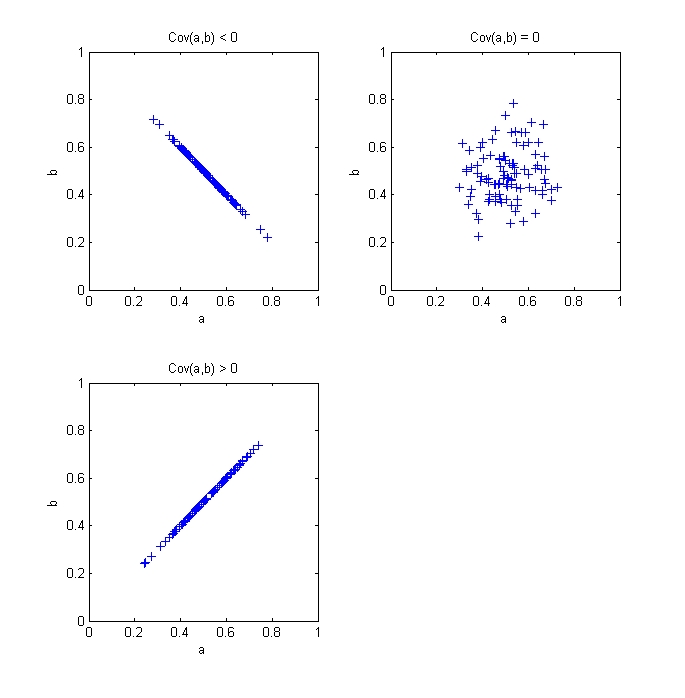
\includegraphics[scale=0.60]{img/correlations.png}
\caption{Three types of correlations between $a$ and $b$}
\end{figure}

\newpage
We can now measure what happens with Var($ab$) when $\mbox{Cov}(a,b) \neq 0$ (thus, when $a$ and $b$ are dependent). Figure~\ref{fig:varab} illustrates that when Cov($a,b$) rises, so does Var($ab$). Also, it is clear that this relation can be approximated by a linear function, as long as the sample sizes of $a$ and $b$ are big enough (see figure~\ref{fig:varabss100}).

\begin{figure}[h]
\centering
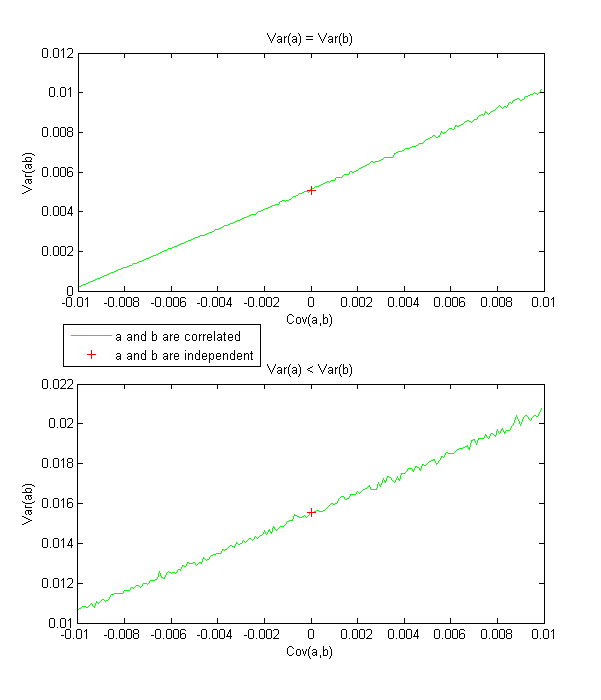
\includegraphics[scale=0.70]{img/varabss50000.png}
\caption{The effect of covariance between $a$ and $b$ on Var($ab$) (sample size: 50\,000)}
\label{fig:varab}
\end{figure}

\newpage
\begin{figure}[h]
\centering
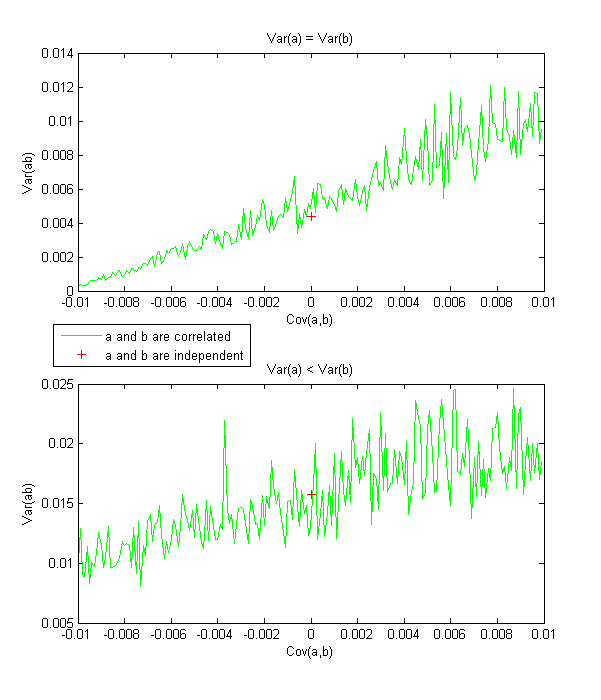
\includegraphics[scale=0.70]{img/varabss100.png}
\caption{The effect of covariance between $a$ and $b$ on Var($ab$) when the size of the samples is small (sample size: 100)}
\label{fig:varabss100}
\end{figure}

If we consider again expression~\ref{eq:nbsimplified}, we can say that:

\begin{itemize}
\item $a=\hat{P}(X_1|Y=y)$
\item $b=\hat{P}(X_2|Y=y)$
\end{itemize}

such that

\begin{eqnarray*}
\mbox{Var}(ab)&=&\mbox{Var}\big(\hat{P}(Y=y|x)\big)\\
&\propto& \mbox{Var}\big( \hat{P}(X_1|Y=y)\,\hat{P}(X_2|Y=y)\big)
\end{eqnarray*}
Based on figure~\ref{fig:varab} and \ref{fig:varabss100}, we can expect that when the prior estimates $\hat{P}(X_1|Y=y)$ and $\hat{P}(X_2|Y=y)$ have a positive (negative) covariance, the variance of $\hat{P}(Y=y|x)$ will increase (decrease). This expectation is also expressed in equation~\ref{eq:diffdepindepapprox}, which approximates the relation between Cov$\big (\hat{P}(X_1|Y=y),\hat{P}(X_2|Y=y)\big)$ and Var$\big (\hat{P}(X_1|Y=y)\,\hat{P}(X_2|Y=y)\big)$. However, when the sample size of $\hat{P}(X_1|Y=y)$ and $\hat{P}(X_2|Y=y)$ (and therefore the size of the bagging ensemble) is not very large, this relation becomes very unreliable. This effect is illustrated in figure~\ref{fig:varabss100}.  If we translate these observations to sampling schemes (1) NBS and (2) bootstrapping, we can make the following statements. In sampling scheme (2), we know that random variables $\hat{P}(X_1|Y=y)$ and $\hat{P}(X_2|Y=y)$ are not independent, and that the estimates of the dependencies are unreliable when there is a lack of training data. We showed that Naive Bayes Sampling removes all feature dependencies, with the result that the \textbf{variance} of $\hat{P}(Y=y|x)$ will decrease (increase) when the covariance between $\hat{P}(X_1|Y=y)$ and $\hat{P}(X_2|Y=y)$  in the original dataset is positive (negative). This means that if we have positive covariance, we better follow the independence sampling scheme (1) in order to reduce the variance of our (test) predictions. Now, if the two features are indeed dependent, introducing artificial independence has an effect on the \textbf{bias} of the prediction error as well. In a Naive Bayes classifier, the bias of the estimate $\hat{P}(Y=y|x)$ is given by:
\begin{eqnarray}
\mbox{Bias}\,(\hat{P}(Y=y|x)) = E(\hat{P}(Y=y|x)) - P(Y=y|x)\label{eq:bias}
\end{eqnarray}
It should be clear that the outcome of $E(\hat{P}(Y=y|x))$ is different when we apply Naive Bayes Sampling and Bootstrapping on a dataset that is not feature independent. Since we do not know $P(Y=y|x)$, it is hard to predict for what sampling scheme and under what conditions the bias, as given in expression~\ref{eq:bias}, will be smaller. 
 What we do know is that in some situations, the variance of the estimate decreases when we apply Naive Bayes Sampling. Hence, in order to choose between Naive Bayes Sampling and Bootstrapping, we advise comparing both techniques and to choose that implementation which results into a better performance on the considered dataset.
 
Although the exact impact of Naive Bayes Sampling is not clear, we can motivate its use as follows. We know that the independence assumptions on which Naive Bayes classifiers are based, almost never hold for natural data sets. Because of this reason, machine learning and information retrieval focused on three kind of strategies~\cite{lewis98}: (1) attempts to produce better classifiers by relaxing the independence assumption, (2) modifications of the features to make the independence assumption more true, and (3) attempts to explain why the independence assumption isn't really needed anyway.

Clearly, Naive Bayes Sampling implements the second strategy by imposing feature independency on the dataset. Other approaches that implement this strategy can mainly be found in information retrieval~\cite{booleanqueries}~\cite{bayesianinference}~\cite{harper78eval}~\cite{Turtle91evaluationof}~\cite{Rijsbergen77}.   
Up to this moment, the effectiveness improvements yielded by these approaches is rather small. Moreover, the nature of their impact is more complex than might be guessed~\cite{Church95oneterm}. The implications of Naive Bayes Sampling illustrate this problem. As a result, we show the performance of Naive Bayes Sampling by a number of experiments in chapter~\ref{experiments}. In order to obtain a full understanding in the differences between Naive Bayes Sampling and Bootstrapping, more research is required.


\begin{figure}[h]
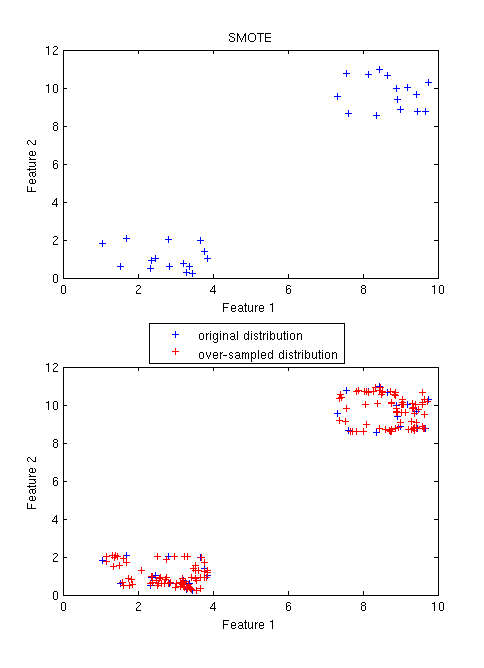
\includegraphics[scale=0.65]{img/SMOTE_featureSampling.png}
\caption{This figure shows how SMOTE emphasizes the generation of synthetic examples within existing minority clusters. The parameter $k$ influences how strict these clusters have to be interpreted, and therefore also the generalization process of the learning algorithm. In the first image, a possible 2-dimensional minority distribution is displayed. This distribution clearly shows two clusters of minority instances, namely one in the bottom left corner, and one in the top right corner. In the second image, the same distribution is displayed (blue), together with an over-sampled distribution by applying the SMOTE technique (red).}
\label{fig:SMOTE}
\end{figure}

\begin{figure}[h]
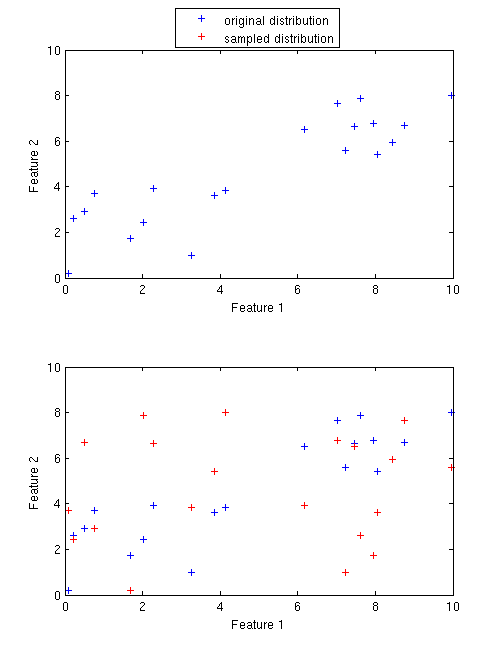
\includegraphics[scale=0.75]{img/nb_featureSampling.png}
\caption{This figure illustrates the effect of sampling with the introduced sampler in section~\ref{rnb-approach}. In the first image, a possible 2-dimensional minority distribution is displayed. This distribution clearly shows two clusters of minority instances, namely one in the bottom left corner, and one in the top right corner. In the second image, the same distribution is displayed (blue), together with a possible synthetic over-sampled distribution (red). This distribution however does not form two clusters anylonger, and is scattered over the joint distribution of the feature space.}
\label{fig:NBS}
\end{figure}




\section{Conclusion}\label{rnb-conclusion}
Experiment results in section~\ref{exp-rnb} show that the introduced approach (RNB-FvB) clearly outperforms current approaches to class imbalance, especially when the datasets contain a large amount of nominal features. Although it is hard to predict how the bias changes when applying RNB-FvB, previous section showed that a positive covariance between the features decreases the variance. As a result, RNB-FvB allows to increase the stability of bagging ensembles when the features have a positive covariance. In order to know when Naive Bayes Sampling outperforms Booststrapping, we advise comparing both techniques by means of stratified 10-fold cross-validation.

Despite of the many benefits, some backdraws hinder the implementation of RNB-FvB. First of all, the sampling process consumes a lot of time (and memory), especially due to the implemented EM-algorithm for numeric features. When a high number of samples needs to be created, it might therefore be more appropriate to undersample the majority class first. A second problem relates to the fact that the introduced sampler can only successfully be implemented with a Naive Bayes classifier (due to the imposed feature independence). This restriction however logically follows from the applied sampling scheme NBS, which is exactly developed to improve cooperation with a Naive Bayes classifier. 

Hence, the restrictions of NBS allow to improve the stability and reliability of a bagging ensemble of Naive Bayes classifiers (RNB-FvB). Also, it is clear that not only all assumptions in this ensemble meet each other, but are moreover validated (due to the imposition of feature independence). This is probably the main reason why RNB-FvB outperforms techniques like cost-sensitivity, SMOTE, Bagging for Imbalanced Datasets and MetaCost.







%-------------------------------------------------------------------------------------------------------------------
% EXPERIMENTS
%-------------------------------------------------------------------------------------------------------------------
\chapter{Experiments}\label{Experiments}
In this chapter, we present the experiment results of (1) the discussed approaches in chapter~\ref{imbalanced} and (2) the proposed approach in chapter~\ref{newapproach}. These experiments are performed on a number of UCI datasets, (presented in section~\ref{uci-ds}) and a medical dataset provided by KULeuven (presented in section~\ref{ill-ds}). In section~\ref{theclassifiers}, we give an overview of the classifiers used in (1).  Afterwards, we present the actual experiment results of (1) and (2) in section~\ref{compex} and~\ref{exp-rnb}.

%-------------------------------------------------------------------------------------------------------------------
% UCI DATASETS
%-------------------------------------------------------------------------------------------------------------------
\section{UCI datasets}\label{uci-ds}
The UCI Machine Learning Repository (\url{http://archive.ics.uci.edu/ml/}) is a collection of databases, domain theories, and data generators that are used by the machine learning community for the empirical analysis of machine learning algorithms. Datasets which were used in these tests are the following:

\begin{itemize}
\item \textbf{Breast-cancer}: the breast cancer domain was obtained from the University Medical Centre, Institute of Oncology, Ljubljana, Yugoslavia (1988). Thanks go to M. Zwitter and M. Soklic for providing the data. The data set includes 85 instances of one class (\textit{recurrence-events}) and 201 instances of another class (\textit{no-recurrence-events}). The instances are described by 9 attributes, of which all are nominal. 

\item \textbf{Hepatitis}: the hepatitis domain was donated by G. Gong, Carnegie-Mellon University, Ljubljana, Yugoslavia (1988). The data set includes 32 instances of one class (\textit{die}) and 123 instances of another class (\textit{live}). The instances are described by 19 attributes, of which 6 are numeric and 13 are nominal.

\item \textbf{Sick}: this dataset conciders Thyroid disease records supplied by the Garavan Institute and the New South Wales Institute (J. Ross Quinlan), Sydney, Australia. The dataset includes 231 instances of one class (\textit{sick}) and 3541 instances of another class (\textit{negative}). The instances are described by 29 attributes, of which  7 are continuous and 23 are discrete.

\item \textbf{Liver-disorders}: This dataset contains blood tests (taken from male individuals) which are thought to be sensitive to liver disorders that might arise from excessive alcohol consumption. The dataset includes 145 instances of one class and 200 instances of another class. The instances are described by 6 attributes, of which all are continuous.
\end{itemize}

\begin{table}[h]
\centering  
\begin{tabular}{ l | r r r r | r r r|}       
& \multicolumn{4}{c}{Instances} & \multicolumn{3}{c}{Features}\\                               
Dataset & Total & Class 1 & Class 2 & C1/C2 & Total & Nominal & Numeric\\
\hline
Breast-cancer & 286 & 85 & 201 & 0.423 & 9 & 9 & 0\\
Hepatitis & 155 & 32 & 123  & 0.260 & 19 & 13 & 6\\
Sick & 3772 & 231 & 3541 & 0.065 & 29 & 22 & 7\\
Liver-disorders & 345 & 145 & 200 & 0.725 & 6 & 0 & 6\\
\hline

\end{tabular}
\label{tab:PPer}
\caption{Summary of classifier performance} % title name of the table
\end{table}


%-------------------------------------------------------------------------------------------------------------------
% CEBAM DATASET
%-------------------------------------------------------------------------------------------------------------------
\section{KULeuven dataset}\label{ill-ds}
The dataset provided by KULeuven considers the problem of discovering serious infections in children~\cite{buntinx}~\cite{symptoms}. This dataset describes two different classes of which the class of interest (the positive class) describes children who have a serious infection for which hospitalisation is necessary. This class is heavily underrepresented compared to the negative class, describing the children for which no hospitalisation was necessary. As a result, we can speak of a typical imbalanced dataset. 

\subsection{The Problem}\label{ill-problem}
The study from which the discussed dataset is derived, regards the diagnosis of serious infections in children. These infections are sepsis, meningitis, pneumonia, pyelonephritis, osteomyelitis, and cellulitis, and are associated with considerable mortality and morbidity. As an example, the mortality of meningococcal disease can be as high as 25\% and approximately 7\% of children who survive bacterial meningitis suffer from hearing loss.  In Flanders, infectious diseases are responsible for 8.0\% of all deaths in children under the age of 1 year, and for 13.6\% of deaths in children aged between 1 and 14 years, comparable to death rates previously reported in the UK.  Although the majority of infections presented to the general practitioner is not serious and the initial presentation of serious and non-serious infections can be similar, early diagnosis of a serious infection is important to avoid delay in treatment and improve prognosis. In addition, diagnosis can be very hard since children present themselves at an early stage of the disease, when signs and symptoms of serious and non-serious infections appear similar. The concerning study included children aged 0-16 years with an acute illness for a maximum of 5 days consecutively~\cite{symptoms}. Signs and symptoms were recorded and compared to the final outcome of these children (a serious infection for which hospitalisation was necessary). The resulting dataset contains a total of 3981 children, of which 31 were admitted to hospital with a serious infection (0.78\%). 

\subsection{Features}
The following features were included in the classification task:
\begin{itemize}
\item Age, Gender, Temperature (the highest body temperature measured by the parents or the physician. Before analysis, 0.5°C was added to temperatures in the axilla, or with a tympanic thermometer), Type of consultation (home visit or office), Duration illness (total duration of the illness, in hours), Child seriously ill (perception of the physician at moment of consultation), Chronical condition present, Chronical condition type, Refer pediater, Refer urgency
\item \textbf{Observations}: Irritated, Drowsy, Unconscious, Unconsolable, Cry, Moan, Laugh, Different (a statement by the parents that this illness was different from previous illnesses)
\item \textbf{Anamnesis}: Urinary tract infection, Headache, Vomiting, Diarrhoea, Eat Drink Normally, TummyAche, Cough, Breathing (any change as compared to normal breathing), Urin, Somnolent, Incoherent
\item \textbf{Physical Examination}: Meningeal irritation (the presence of neck stiffness, Kernig's sign, Brudzinsky's sign 1 or 2, and a bulging fontanelle, or irritability on manipulation of the head or legs in children aged younger than 1 year old), Petechiae (in cases of a non-blanching rash), Rash, Tachypnoea (breathing frequency of 40 or greater per minute), Dyspnoea (difficult or laboured breathing), Creptitations, Decreased breathing sounds, Cyanosis, Impaired peripheral circulation (when capillary refill more than 3 sec), Convulsions, Weight loss, Dehydration, Something Wrong (a subjective feeling of the physician that things were not right)
\item \textbf{Evaluation}: Serious without GE bronch: serious infections were defined as admission to hospital with one of the following infections: pneumonia (infiltrate on chest X-ray), sepsis (pathogen in haemoculture), viral or bacterial meningitis (pleocytosis in cerebrospinal fluid and identification of bacteria or a virus), pyelonephritis (105/ml or more pathogens of a single species and white blood cells in urine and serum C-reactive protein elevation), cellulitis (acute, suppurative inflammation of the subcutaneous tissues).  Sepsis and Meningitis were combined a priori into one diagnostic category.
\end{itemize}

\newpage
\paragraph*{Coding}\label{ill-coding}
In order to allow a compacter visualisation of the data, the different features were coded as follows:

\begin{tabular}{llll}
\cr
1 & Age & 21 & Anm Cough\\
2 & Gender & 22 & Anm Breathing\\
3 & Duration Total & 23 & Anm Urin\\
4 & Child seriously ill? & 24 & Anm Somnolent\\
5 & Chronical Condition Present? & 25 & Anm Incoherent\\
6 & Temperature & 26 & PE Meningeal Irritation\\
7 & Obs Irritated & 27 & PE Petechiae\\
8 & Obs Drowsy & 28 & PE Rash\\
9 & Obs Unconscious & 29 & PE Tachypnoea\\
10 & Obs Unconsolable & 30 & PE Dyspnoea\\
11 & Obs Cry & 31 & PE Crepetitations\\
12 & Obs Moan & 32 & PE Decreased Breathing Sounds\\
13 & Obs Laugh & 33 & PE Cyanosis\\
14 & Obs Different & 34 & PE PerCirc\\
15 & Anm Urinary Tract Infection & 35 & PE Convulsions\\
16 & Anm Headache & 36 & PE Weight Loss\\
17 & Anm Vomiting & 37 & PE Dehydr\\
18 & Anm Diarrhoea & 38 & PE Something Wrong\\
19 & Anm Eat Drink & 39 & Serious (without GE bronch)\\
20 & Anm TummyAche &  & \\
\cr
\end{tabular}

\paragraph*{Values}
The nominal features 7 to 39 can take three possible values, and are coded as \{0=yes, 1=no, 2=don't know\}. Features 2, 4, 5 and 38 can only take two values, and are coded as \{0=boy, 1=girl\} resp. as \{0=yes, 1=no\}.

\subsection{Dimensionality Reduction}\label{dimred}
In order to get some insight into how the data is distributed, dimensionality reduction techniques can be applied. These techniques regard the reduction of the number of features in a dataset. Hence, it becomes possible to compress the original 37-dimensional instance space into a space of only 2 dimensions, thereby making visualisation of the data possible. In this subsection, we apply several famous techniques and compare their results, such that a well-founded view of the data can be formulated. Most of these techniques are performed in Matlab by making use of the built-in functions and a toolbox provided by Laurens Van der Maaten~\cite{matlabToolbox}. \\
Before dimensionality reduction is performed, the data is preprocessed such that it becomes clear of missing values and irrelevant features.  Features \textit{Type of consultation} and \textit{Chronical condition type} (because of many missing values) are removed for this purpose. Missing values in other features are replaced by the mean (numerical features), or by the \textit{don't know} value (nominal features). The result is a new dataset of size 3\,981\,x\,37. Notice that these preprocessing techniques are not applied for the classification task.\\

\newpage
One of the most known dimensionality reduction techniques is \textbf{Principal Component Analysis} (PCA). In general, PCA performs a (linear) transformation on the original data, such that a maximum amount of its variance is explained by a minimum amount of features in the new, transformed, data. The features of the transformed data are called \textit{principal components}, and are ordered in descending order by the amount of variance they explain. Reducing the number of dimensions can then simply be achieved by removing the principal components explaining the least amount of variance. Usually, the explained variance of the principal components is illustrated in a scree plot. A scree plot is a simple line segment plot that shows the fraction of total variance in the data as explained or represented by each principal component. Therefore, a scree plot illustrates how much a certain dataset can be compressed without losing too much information (variance).

The following image illustrates different scree plots of the \textit{ill children} dataset. In order to have an idea what data contains more information, PCA is performed to the whole dataset (black), a random dataset of 100\,000 x 38 examples (black dotted) and a subset containing only the \textit{ill} examples (blue).\\

\begin{figure}[h]
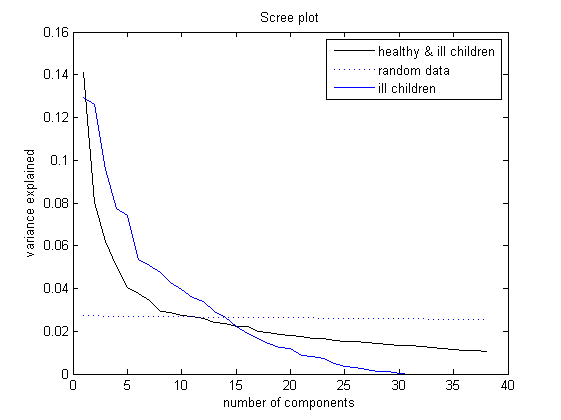
\includegraphics[scale=0.95]{img/pca_scree.png}
\end{figure}

In the illustration, we can see that the first component explains 14.12\% of the variance in the data, and that in order to explain more than 65\% (65.54\%), 15 out of the 38 components are needed.  Also, it seems that the variance within the \textit{ill} examples can be captured in a better way: the first component only explains 12.93\% of the variance in the data, but 65.52\% of the variance can be captured by 'only' 8 components.
The scree plot clearly shows that compression of the data is very costly, which means that most of the original features do not contain a lot of information (but clearly more than random data).

When we only keep the two most informative principal components, we can plot the resulting (transformed) dataset in a 2D-plot. The following illustration shows the resulting visualisation, where the positive (\textit{ill}) and negative (\textit{healthy}) examples are marked with different symbols. Although the plot suggests the presence of some clusters within the data, it is clear that the positive examples are scattered completely amongst the distribution of the negative examples and that no clear separation exists at this level.

\begin{figure}[h]
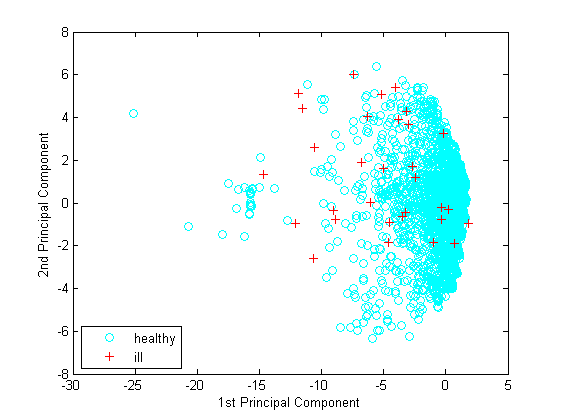
\includegraphics[scale=0.95]{img/pca_space.png}
\end{figure}


Another approach to analyse the data, is to find out how close features are related to each other. This can for example be achieved with \textbf{Multidimensional Scaling} (MDS), another linear technique with a similar aim as PCA.  MDS finds a low-dimensional projection of the data such as to preserve, as closely as possible, the pairwise distances between data points.  In the case where the distances are Euclidian, it gives equivalent results to PCA~\cite{bishop}.
We can obtain a distance matrix of the dataset by calculating its correlation matrix and transforming it such that the elements represent dissimilarities (in stead of similarities). When we perform MDS on this matrix, we can plot the (dis)similarities between all the features in a 2D-plot.\\
The following illustration shows the (dis)similarities between the features of the \textit{ill children} dataset after performing MDS. The features are labeled by an ID explained earlier in~\ref{ill-coding}.


\newpage

%\begin{landscape}
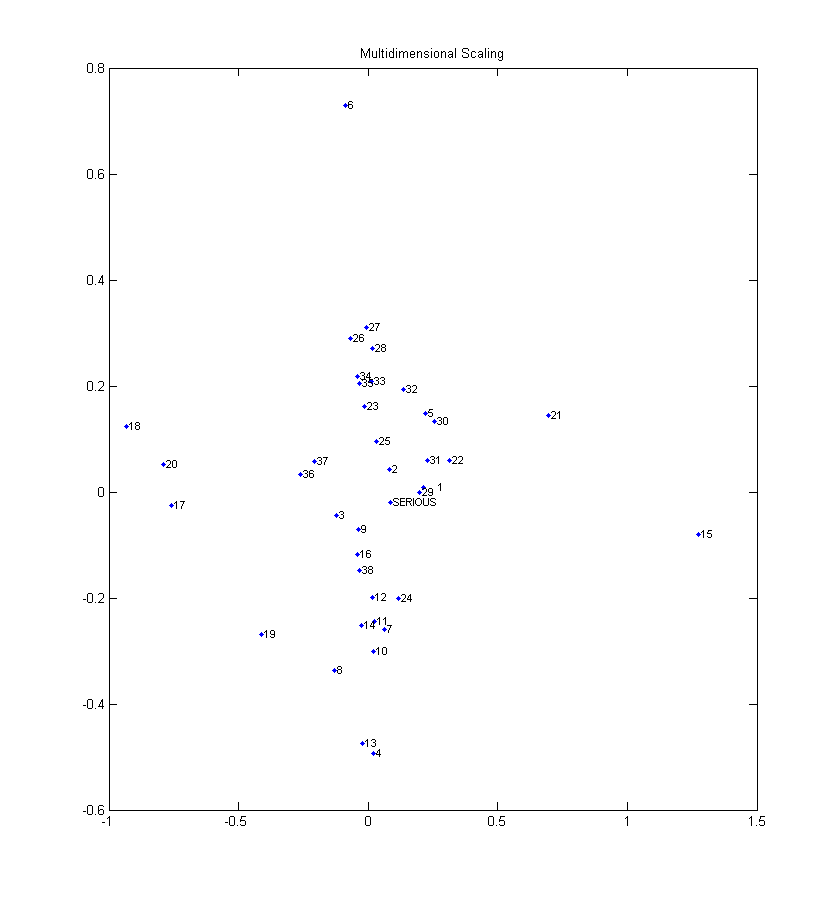
\includegraphics[scale=0.70]{img/mds_corr_stdN.png}
%\end{landscape}

Summarized, we can say that the data does not contain a high degree of correlated features, and that there exists no clear separation of the positive instances. Since the minority data is moreover described by more dimensions than it is populated by examples, we can expect difficulties when modeling the data distribution for sampling purposes. Important features regarding the final outcome seem to be: tachypnoea, age, gender, the total duration of the illness, unconsciousness, headache, Something Wrong, breathing problems, crepetitations and incoherentness. Less important features are: temperature, Urinary Tract Infection, diarrhoea, tummyache, vomiting, and cough.


%-------------------------------------------------------------------------------------------------------------------
% THE CLASSIFIERS
%-------------------------------------------------------------------------------------------------------------------
\newpage
\section{Learning Algorithms}\label{theclassifiers}
In this section we give a brief overview of the learning algorithms that are used in the experiments. With the exception of CART, these algorithms are provided by Weka, a Java Opensource (GNU General Public License) software collection of machine learning algorithms for data mining tasks (\url{http://www.cs.waikato.ac.nz/ml/weka}). The experiments of CART are performed with \textit{rpart} (\url{http://cran.r-project.org/web/packages/rpart/}).

\subsection{J48}
J48 is a learning algorithm for generating a pruned or unpruned C4.5 decision tree~\cite{J48}. The main approach of these classifiers was discussed in section~\ref{classifier-example}. Additionally to explained capabilities, J48 is able to evaluate continuous features and to handle missing feature values. An important modeling choice in this learning algorithm regards the \textit{confidence factor}, which is used for pruning (smaller values incur more pruning).

\subsection{JRip}
JRip is an implementation of Repeated Incremental Pruning to Produce Error Reduction (RIPPER), an optimized version of the propositional rule learner IREP. The learning algorithm consists of three stages. In the first stage, rules are growed and pruned using the concept of information gain. In the second stage, generated rules are examined and optimized for generalization purpose (using the concept of Description Length). Finally, rules that hinder generalisation are deleted in the third stage. An important modeling choice in J48 defines whether decision rules are pruned or not.~\cite{jrip}

\subsection{Naive Bayes}
The Naive Bayes algorithm is a learning algorithm based on Bayes rule, that assumes the features $X_1 \ldots X_m$ are all conditionally independent of one another, given $Y$. The value of this assumption is that it dramatically simplifies the representation of $P(x|y)$, and the problem of estimating it from the training data. In order to deal with continuous features, two approaches are suggested. The first approach involves density estimation by a Gaussian distribution. The second approach involves density estimation by a nonparametric kernel~\cite{John95estimatingcontinuous}. Naive Bayes learning turns out to do surprisingly well in a general-purpose learning algorithms; the boosted version is one of the most effective general-purpose learning algorithms.  Naive Bayes scales well to very large problems: with $n$ Boolean features, there are just \(2n+1\) parameters to estimate, and no search is required to find the maximum-likelihood Naive Bayes hypothesis.  Finally, Naive Bayes learning has no difficulty with noisy data and can give probabilistic predictions when appropriate~\cite{Russell07Artificial}.

\subsection{IBk}
IBk is Weka's implementation for K-nearest neighbor learning (kNN), one of the most basic lazy (or: instance-
based) learning methods. This means that it does not explicitly induce a representation of the target function, but rather stores the training data during the training phase. More specifically, kNN simply retrieves the \(k\) nearest neighbors of a presented instance from training data, and classifies that instance according to a voting scheme that is applied to the classes of these neighbors. Generalisation beyond training data is achieved  according to the assumption that the classification of a query instance should be oriented on those instances which are nearby in feature space. The parameter \(k\) is a direct lever for adjusting the degree of fit to the training data. As a result, nearest neigbhour (NN) learning algorithms have several benefits:

\begin{itemize}
\item simple representations for concept descriptions
\item low incremental learning costs
\item small storage requirements
\item ability to produce concept exemplars on demand
\item ability to learn continuous functions
\item ability to learn non-linearly separable categories
\end{itemize}

An important backdraw of NN learning algorithms is the fact that they are highly sensitive to noise. For this purpose, an extension has been introduced by Aha \& Kibler, which identifies and eliminates noisy concept description instances~\cite{Aha91instance-basedlearning}.

\subsection{SMO}
Sequential Minimal Optimization (SMO) was introduced by John Platt's~\cite{Platt98machines} in order to train a support vector machine (SVM). SVMs are based on the concept of decision planes that define decision boundaries. In order to allow complex decision boundaries, training instances are rearranged using a set of mathematical functions (kernels) such that they become linearly separable. This mapping technique however implies a complex optimization problem, also known as the quadratic programming (QP) optimization.  SMO breaks this problem into a series of smallest possible QP problems, which are then solved analytically. This avoids using a time-consuming numerical QP optimization as an inner loop. Because matrix computation is avoided, SMO scales somewhere between linear and quadratic in the training set size for various test problems, while the standard chunking SVM algorithm scales somewhere between linear and cubic in the training set size~\cite{Platt98smo}. Weka's implementation normalizes all features by default, globally replaces all missing values and transforms nominal attributes into binary ones.

\subsection{CART}
Classification and Regression Tree analysis (CART)~\cite{Bk1871082462} involves using binary trees for tackling classification and regression problems. Basically, the algorithm calculates at each node of the decision tree which variable is the \textit{most discriminating} (using the Gini index) and constructs at that node a bifurcation of two branches. Instead of employing stopping rules, CART generates a sequence of subtrees by growing a large tree and pruning it back until only the root node is left. Then it uses cross-validation to estimate the misclassification cost of each subtree and chooses the one with the lowest estimated cost. As a result, since multiple trees must be built and pruned, the procedure used for pruning is more complex (and therefore more time consuming) than C4.5's pruning, but tends to produce smaller trees~\cite{oatesJensen97}. This technique has a number of advantages over other classification methods, including multivariable logistic regression. First, it is inherently non-parametric, meaning no assumptions have to be made about the underlying distribution. Secondly, the resulting classifiers summarized in a tree are simpler to interpret than multivariable logistic regression classifiers, making it more practical in a clinical setting. However, it should be noted that CART also has some undesirable properties~\cite{cartLoh}: first, the splitting method is biased towards variables that have more distinct values. Sencondly, the exponential number of splits for categorical variables causes serious computational difficulties when the number of distinct values a variable can take is large and \textit{y} takes more than two values. Finally, the algorithm is also biased towards variables with more missing values.

%-------------------------------------------------------------------------------------------------------------------
% Experiments on existing approaches
%-------------------------------------------------------------------------------------------------------------------
\section{Experiment results of discussed approaches}\label{compex}
In this section, we present the experiment results of discussed approaches in chapter~\ref{imbalanced}, applied on the dataset of KULeuven. We evaluate the classifiers by applying stratified 10-fold cross-validation (which is repeated over 10 randomized runs) and measuring the AUC, sensitivity and specificity. A summary of these experiments can be found in section~\ref{exp-summary}.
%-------------------------------------------------------------------------------------------------------------------
% Cost-sensitivity
%-------------------------------------------------------------------------------------------------------------------
\subsection{Cost-Sensitive Learning}\label{costsensitive}
In this section, we investigate the effect of introducing cost-sensitivity in the discussed classifiers. Cost-sensitivity is obtained by reweighting training instances according to a certain sample ratio (as discussed in section~\ref{cost-sensitivity}). In these experiments, the cost of misclassifying minority instances is gradually increased as such that higher sensitivities can be obtained. In order to have a better view into the effect of increasing costs, misclassification costs are often log-plotted (\textit{log10}). Since Weka does not support CART, another software package (\textit{rpart} - \url{http://cran.r-project.org/web/packages/rpart/}) was used to analyse this learning algorithm. This package allows incorporation of variable and possibly non-symmetric misclassification costs into the splitting rule via prior specification. It should however be noted that \textit{rpart} does not provide cross-validation support for evaluating the actual classifier prediction power (which is not to be confused with the internally used cross-validation in order for classifier selection).


\newpage
\begin{figure}[h]
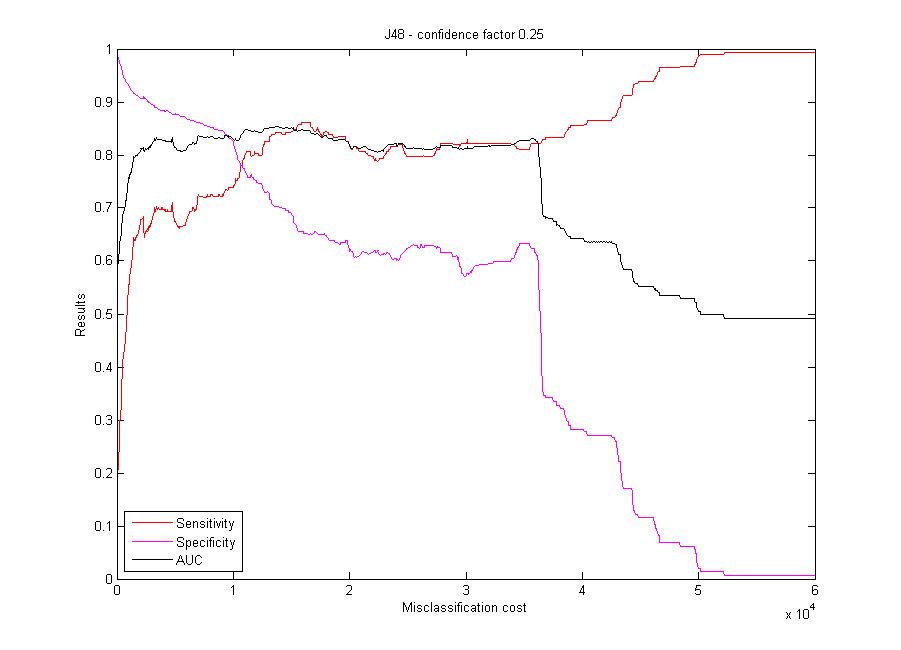
\includegraphics[scale=0.65]{img/J48-confid025.png}
\caption{\textbf{Cost-sensitivity and J48} (confidence factor 0.25) - The classifier resulting into the highest AUC (0.8536) is obtained with a misclassification cost of 13\,250 and yields a sensitiviy of 83.87\% and specificity of 71.44\%. At a misclassification cost of around 36000, a significant drop in specificity and AUC occurs against only a very small increase in sensitivity.}
\end{figure}

\newpage
\begin{figure}[h]
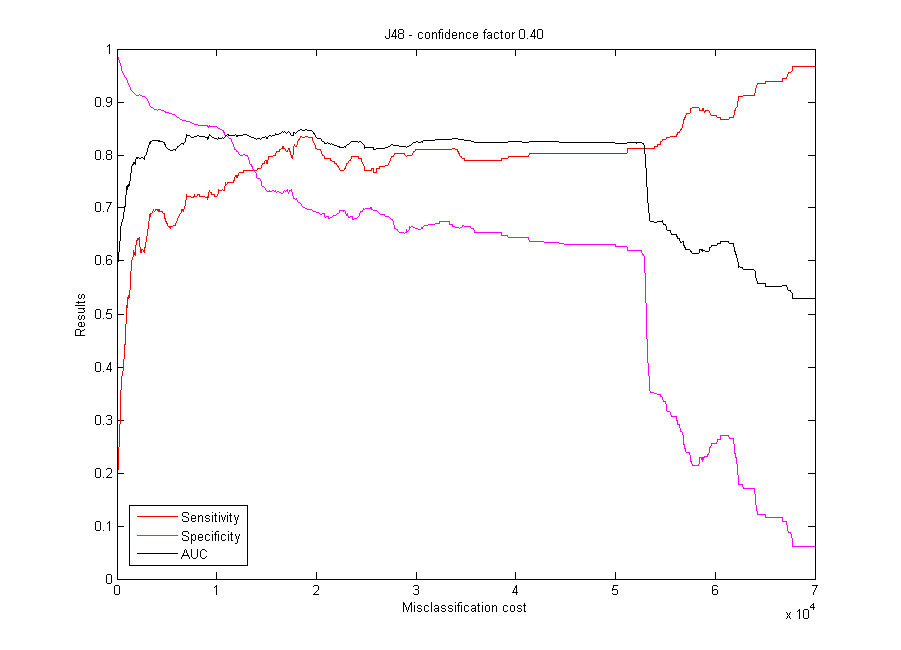
\includegraphics[scale=0.65]{img/J48-confid040.png}
\caption{\textbf{Cost-sensitivity and J48} (confidence factor 0.40) - The classifier resulting into the hightest AUC (0.8487) is obtained with a misclassification cost of 18\,400 and yields a sensitivity of 83.55\% and specificity of 70.81\%.  Again, a significant drop in specificity and AUC against a small increase in sensitivity occurs around a misclassification cost of 53000.}
\end{figure}

\newpage
\begin{figure}[h]
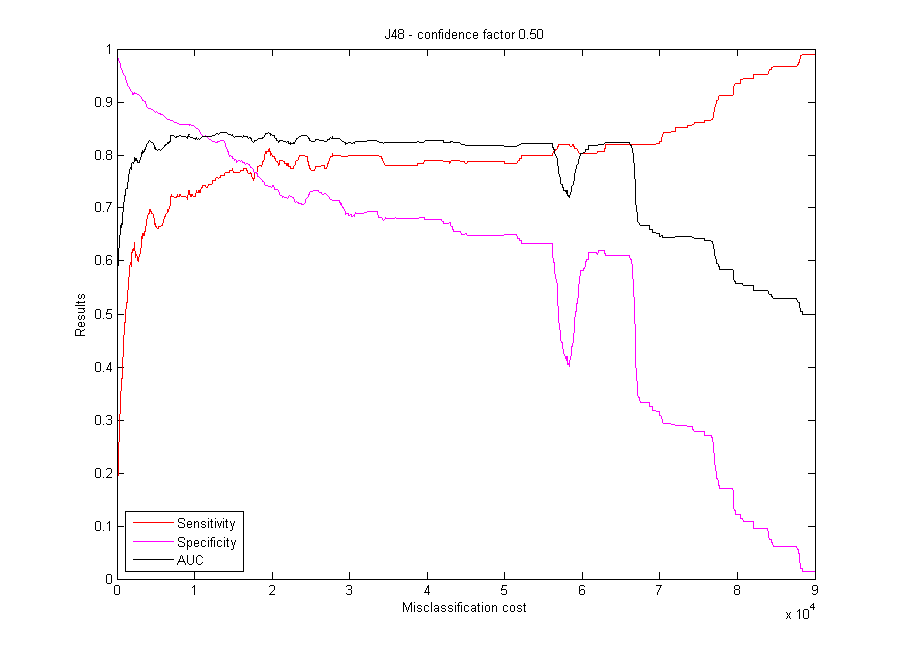
\includegraphics[scale=0.65]{img/J48-confid050.png}
\caption{\textbf{Cost-sensitivity and J48} (confidence factor 0.65) - The classifier resulting into the hightest AUC (0.8431) is obtained with a misclassification cost of 19\,600 and yields a sensitivity of 81.29\% and specificity of 73.93\%.  Two times, a significant drop in specificity occurs which is only recovered once.}
\end{figure}

\newpage
\begin{figure}[h]
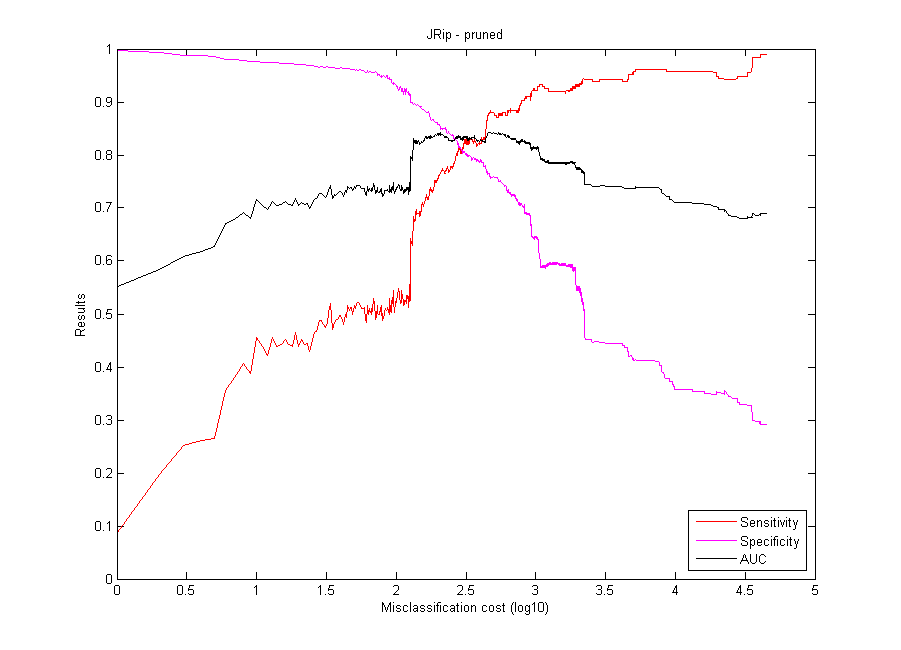
\includegraphics[scale=0.65]{img/jrip.png}
\caption{\textbf{Cost-sensitivity and JRip} (pruned decision rules) - JRip appears to achieve quite fast high sensitivities: at a misclassification cost of 466, a sensitivity of 87.74\% and specificity of 76.50\% is obtained (AUC: 0.8431). Obtaining higher sensitivities however becomes very costly: a sensitivity of 90.32\% is reached at a cost of 787 (specificity: 70.57\%), a higher sensitivity of 94.19\% at cost 2160 (specificity: 51.81\%). To achieve a 99.03\% sensitivity rate, costs have to be increased up to  40\,890, leaving a specificity of only 29.13\%.}
\end{figure}

\newpage
\begin{figure}[h]
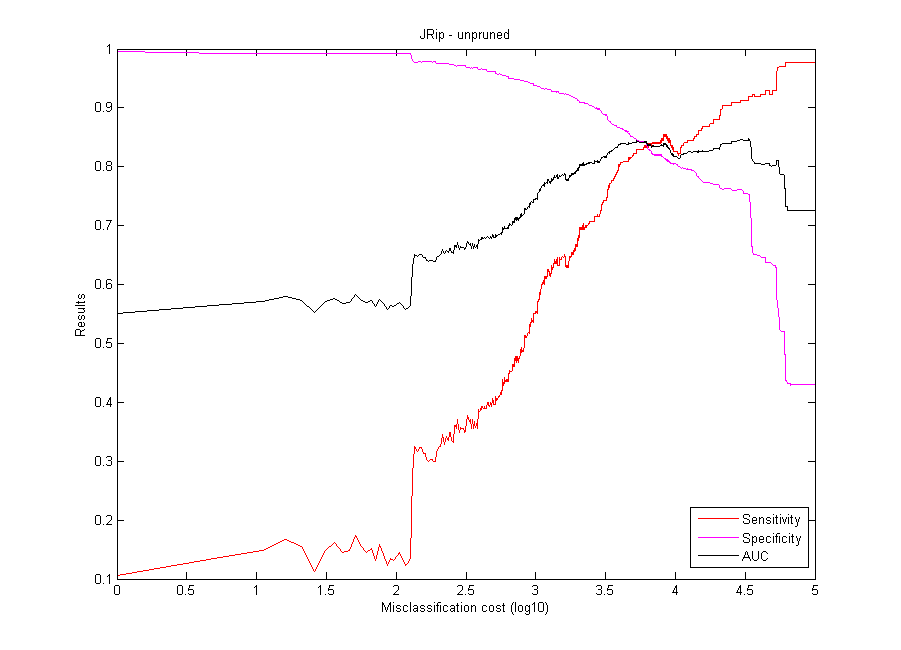
\includegraphics[scale=0.65]{img/jrip-nopruning.png}
\caption{\textbf{Cost-sensitivity and JRip} (unpruned decision rules) - Unpruned decision rules appear to have a positive effect on the sensitivities: at a misclassification cost of 33350, a sensitivity of 91.94\% and specificity of 75.33\% is obtained (AUC: 0.8473). Obtaining higher sensitivities however  becomes very costly: a sensitivity of 94.84\% is reached at a cost of 52985 (specificity: 60.90\%).}
\end{figure}

\newpage
\begin{figure}[h]
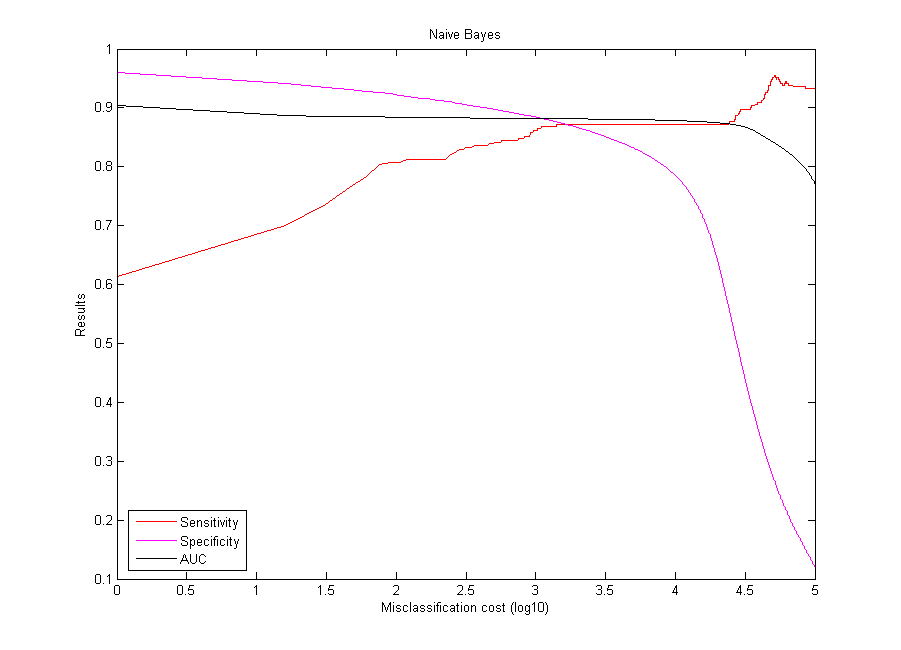
\includegraphics[scale=0.65]{img/naivebayes.png}
\caption{\textbf{Cost-sensitivity and Naive Bayes} (Laplace smoothing) - Experiment results of cost-sensitive learning with Naive Bayes using the Laplace estimate.}
\end{figure}

\newpage
\begin{figure}[h]
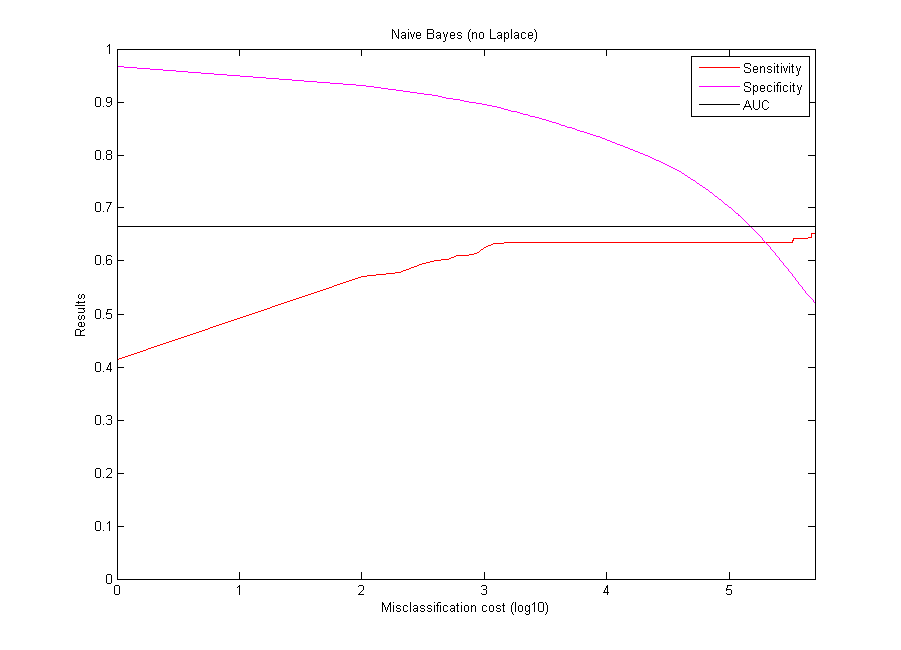
\includegraphics[scale=0.65]{img/naivebayes-nolaplace.png}
\caption{\textbf{Cost-sensitivity and Naive Bayes} (no smoothing) - Experiment results of cost-sensitive learning with Naive Bayes using no smoothing estimate.}
\end{figure}

\newpage
\begin{figure}[h]
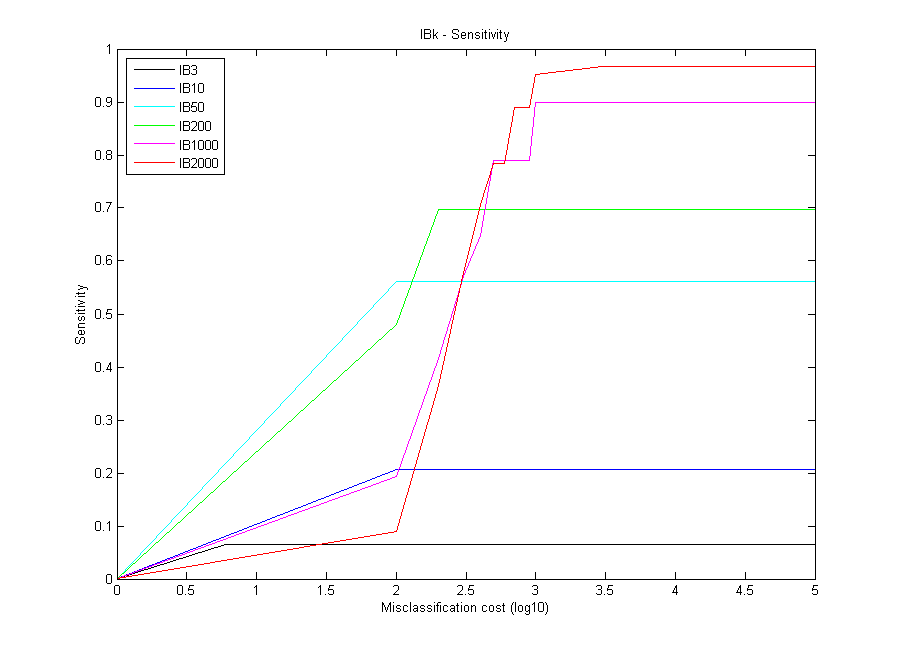
\includegraphics[scale=0.65]{img/IBk_sens.png}
\caption{\textbf{Cost-sensitivity and IBk} (Sensitivities) - Sensitivities mainly seems to be affected by the number of evaluated nearest neighbours, rather than the applied misclassification cost. Although the positive instance weight influences the sensitivity in an early stage, further increase does not lead to any improvements unless the number of nearest neighbours is increased. IB3 reaches a maximum sensitivity of 6.45\%, IB10 20.65\%, IB50 56.13\%, IB200 69.68\%, IB1000 90\% and IB2000 96.77\%.}
\end{figure}

\newpage
\begin{figure}[h]
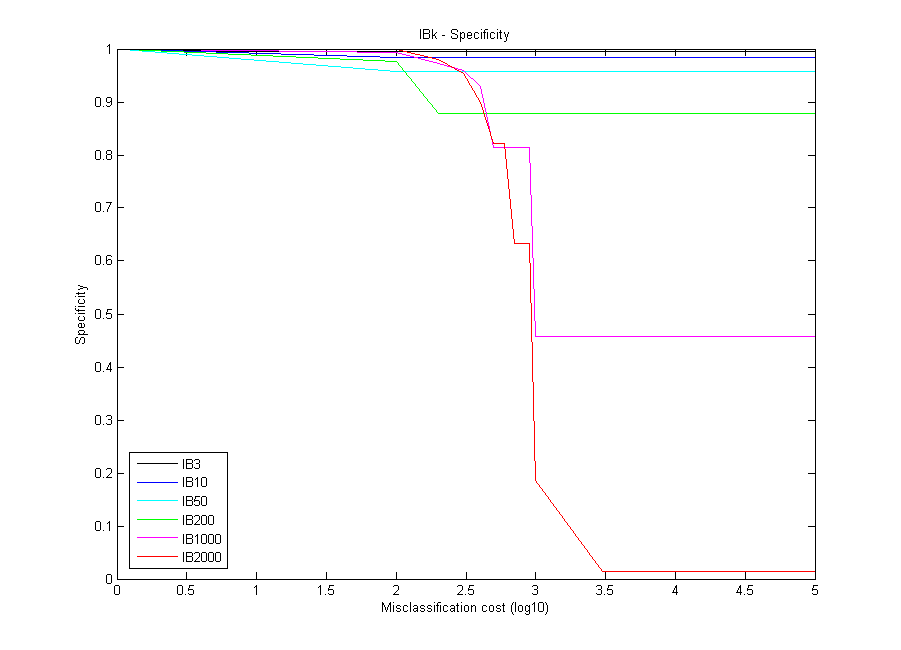
\includegraphics[scale=0.65]{img/IBk_spec.png}
\caption{\textbf{Cost-sensitivity and IBk} (Specificities) - A similar situation as in the sensitivities occurs with the specificities. Once the highest sensitivity is reached, specificities remain steady unless the number of nearest neighbours is increased. At the highest sensitivity of IB3, a specificity of 99.59\% holds, for IB10 98.48\%, for IB50 95.71\%, for IB200 87.77\%, for IB1000 45.66\% and for IB2000 1.48\%.}
\end{figure}

\newpage
\begin{figure}[h]
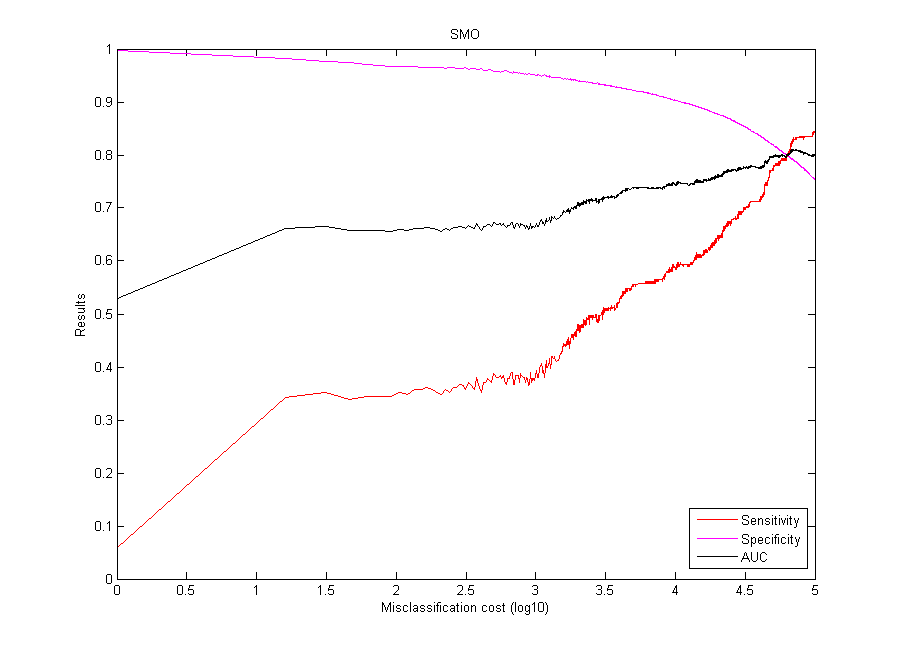
\includegraphics[scale=0.65]{img/smo.png}
\caption{\textbf{Cost-sensitivity and SMO} (complexity parameter $c=1$, linear exponent) - Experiment results of cost-sensitive learning with SMO.}
\end{figure}

\newpage
\begin{figure}[h]
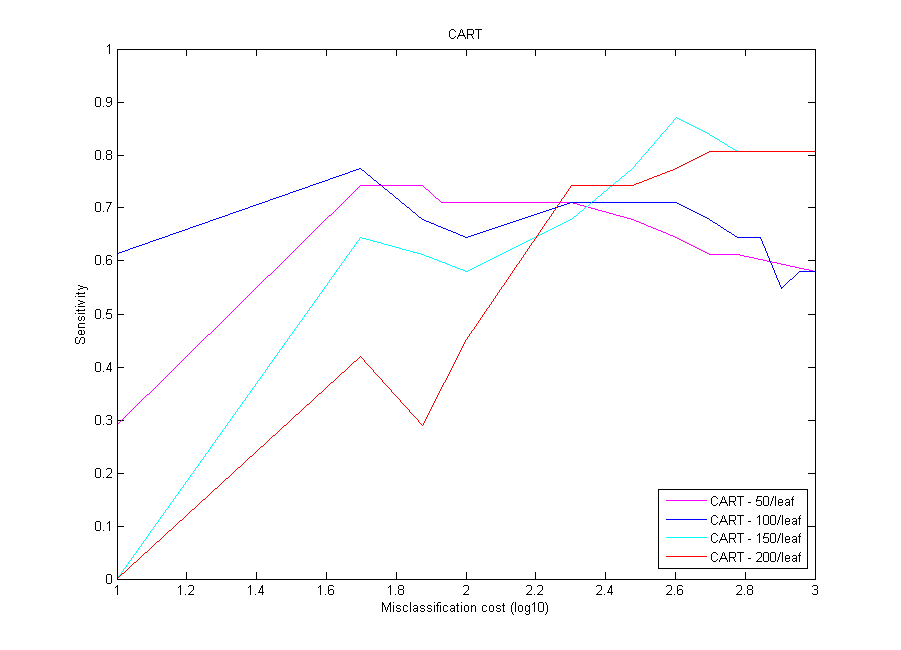
\includegraphics[scale=0.65]{img/CART_sens.png}
\caption{\textbf{Cost-sensitivity and CART}  (Sensitivities) - In this experiment, 4 different types of classifiers were built using a different minimum number of observations (50, 100, 150 and 200) that must exist in a node or a terminal node . Results show that how lower the minimum number of observations in a node or terminal node becomes, how lower the sensitivities become (although the perfomance on the training set increases). }
\end{figure}

\newpage



\begin{figure}[h]
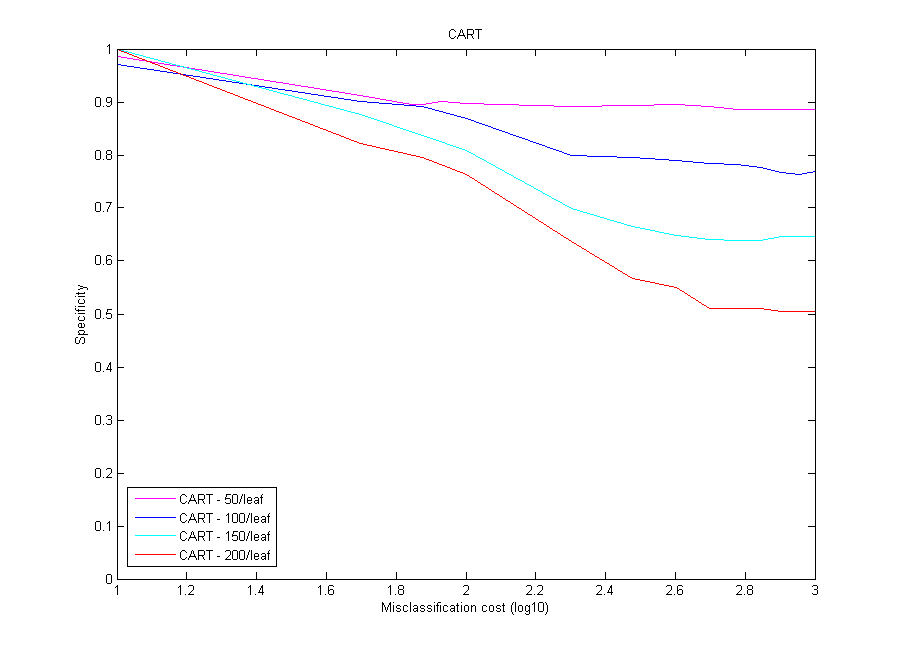
\includegraphics[scale=0.65]{img/CART_spec.png}
\caption{\textbf{Cost-sensitivity and CART} (Specificities) - In the specificities, the cost increase yields less performance degrade when the minimum number of observations in a (terminal) node is low.}
\end{figure}


%-------------------------------------------------------------------------------------------------------------------
% MetaCost
%-------------------------------------------------------------------------------------------------------------------
\newpage
\subsection{MetaCost}\label{exp-metacost}
In this section, we introduce cost-sensitivity by applying MetaCost on the discussed classifiers. In order to keep the number of experiments realistic, we only test those types of classifiers that proved most promising (highest AUC) in cost-sensitivity analysis.  

\begin{figure}[h]
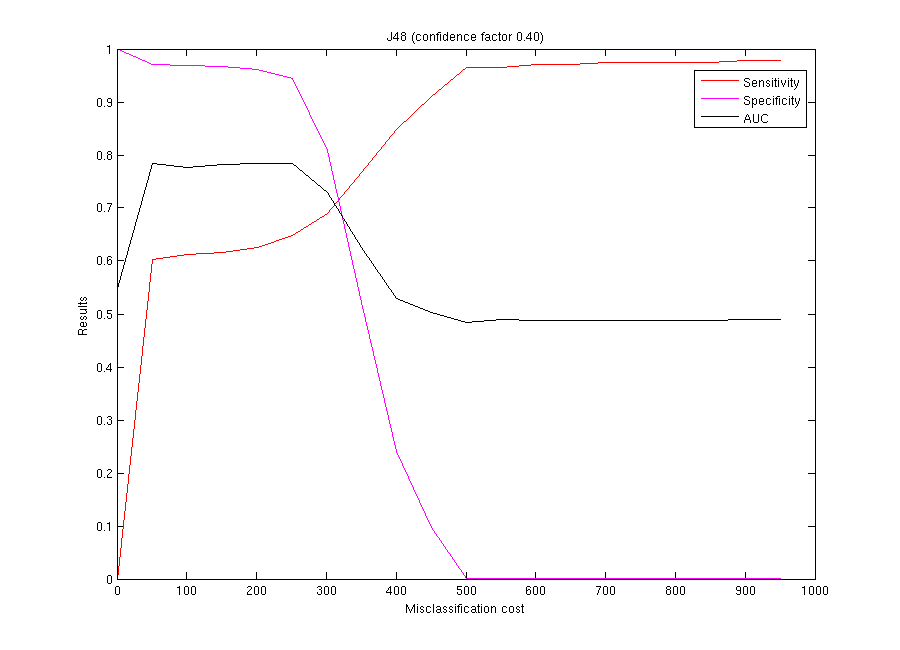
\includegraphics[scale=0.65]{img/MC_J48-confid040.png}
\caption{\textbf{MetaCost with J48} (confidence factor 0.65) - Experiment results of MetaCost with J48. MetaCost allows J48 to achieve a maximum AUC of 0.7846 at a misclassification cost of 251. This classifier yields a sensitivity of 64.84\% and a specificity of 94.51\%. A sensitivity of 90.97\% is achieved using a misclassification cost of 451, and yields a specificity of 9.71\%. Finally, a maximum sensitivity of 97.74\% is obtained together with a specificity of 0.00\%.}
\end{figure}

\newpage
\begin{figure}[h]
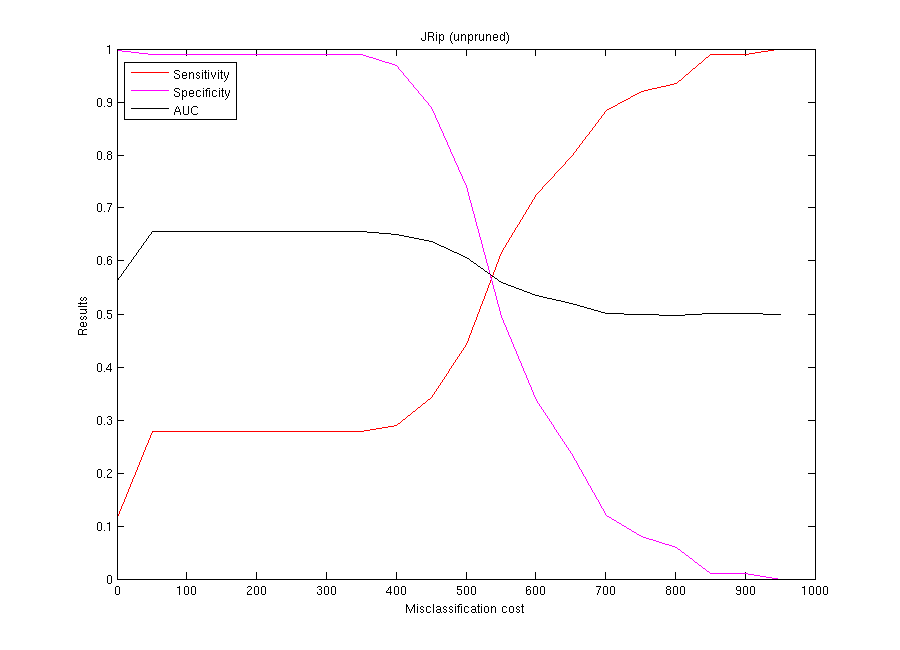
\includegraphics[scale=0.65]{img/MC_JRip-unpruned.png}
\caption{\textbf{MetaCost with JRip} (unpruned decision rules) - Experiment results of MetaCost with JRip. MetaCost allows JRip to achieve a maximum AUC of 0.6565 at a misclassification cost of 51. This classifier yields a sensitivity of 27.74\% and a specificity of 98.87\%. A sensitivity of 91.94\% is achieved using a misclassification cost of 751, and yields a specificity of 7.93\%. Finally, a maximum sensitivity of 100.00\% is obtained together with a specificity of 12.54\%.}
\end{figure}

\newpage
\begin{figure}[h]
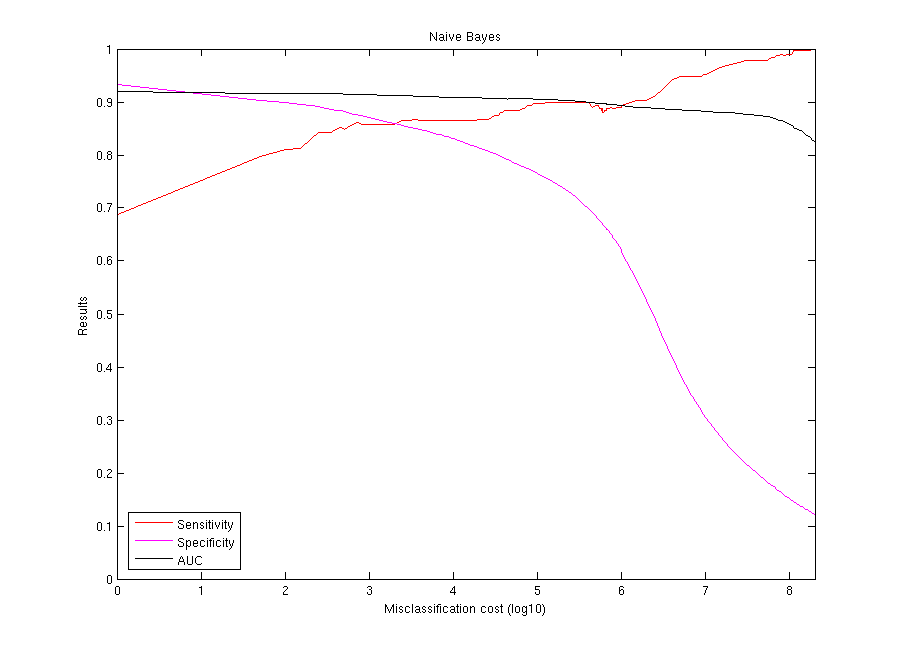
\includegraphics[scale=0.65]{img/MC_Naivebayes.png}
\caption{\textbf{MetaCost with Naive Bayes} (Laplace smoothing) - MetaCost allows Naive Bayes to achieve a maximum AUC of 0.9206 at a misclassification cost of 1. This classifier yields a sensitivity of 68.71\% and a specificity of 93.28\%. A sensitivity of 90.32\% is achieved using a misclassification cost of 1\,500\,000, and yields a specificity of 56.53\%. Finally, a maximum sensitivity of 100.00\% is obtained together with a specificity of 0.00\%.}
\end{figure}

\newpage
\begin{figure}[h]
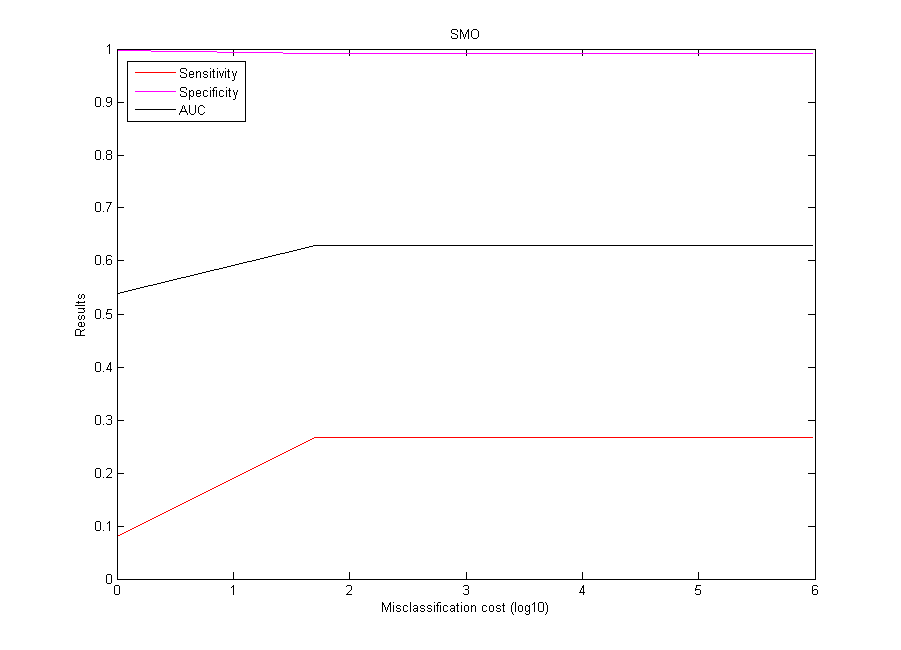
\includegraphics[scale=0.65]{img/MC_SMO.png}
\caption{\textbf{MetaCost with SMO} - MetaCost allows SMO to achieve a maximum AUC of 0.6299 at a misclassification cost of 51. This classifier yields a sensitivity of 26.77\% and a specificity of 99.22\%. When costs are further increased up to 1\,000\,000, no different models are obtained.}
\end{figure}


%-------------------------------------------------------------------------------------------------------------------
% SMOTE
%-------------------------------------------------------------------------------------------------------------------
\newpage
\subsection{SMOTE}\label{exp-SMOTE}
In this section, we apply the Synthetic Minority Over-sampling Technique (SMOTE) using 5 nearest neighbours. In order to keep the number of experiments realistic, we only test those types of classifiers that proved most promising (highest AUC) in cost-sensitivity analysis.

\begin{figure}[h]
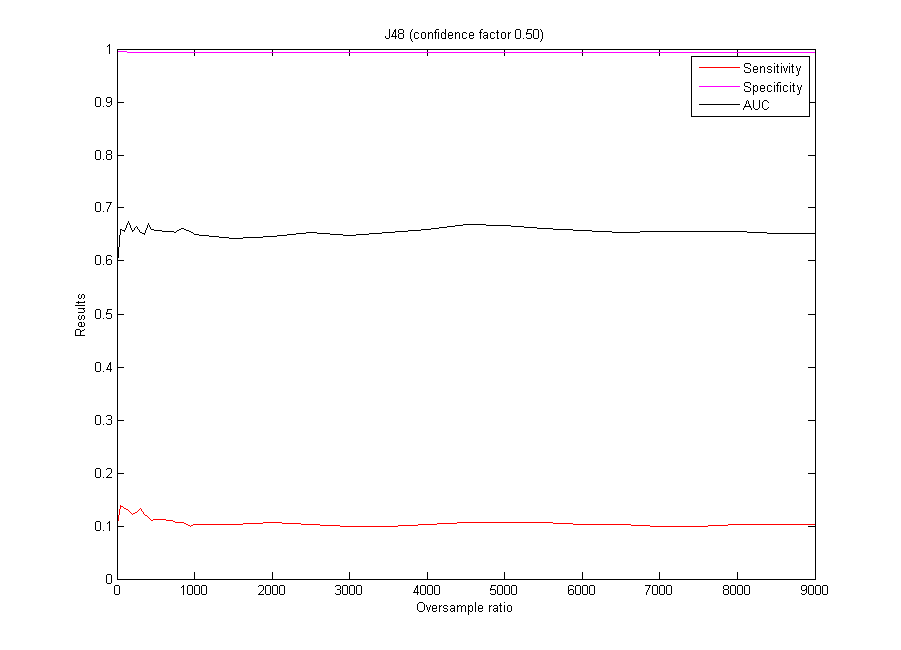
\includegraphics[scale=0.65]{img/SMOTE_J48-confid-050.png}
\caption{\textbf{SMOTE and J48} (confidence factor 0.50) - The generation of synthetic instances seems to have rather a limited/negative effect in favouring the recognition rate of the minority samples. A maximum AUC of 0.6750 is achieved at a  misclassification cost of 150. This classifier yields a sensitivity of 12.90\% and a specificity of 99.33\%. At a misclassification cost of 51, a maximum sensitivity of 13.87\% is obtained (specificity: 99.55\%).
}
\label{fig:exp-smote-j48}
\end{figure}

\newpage
\begin{figure}[h]
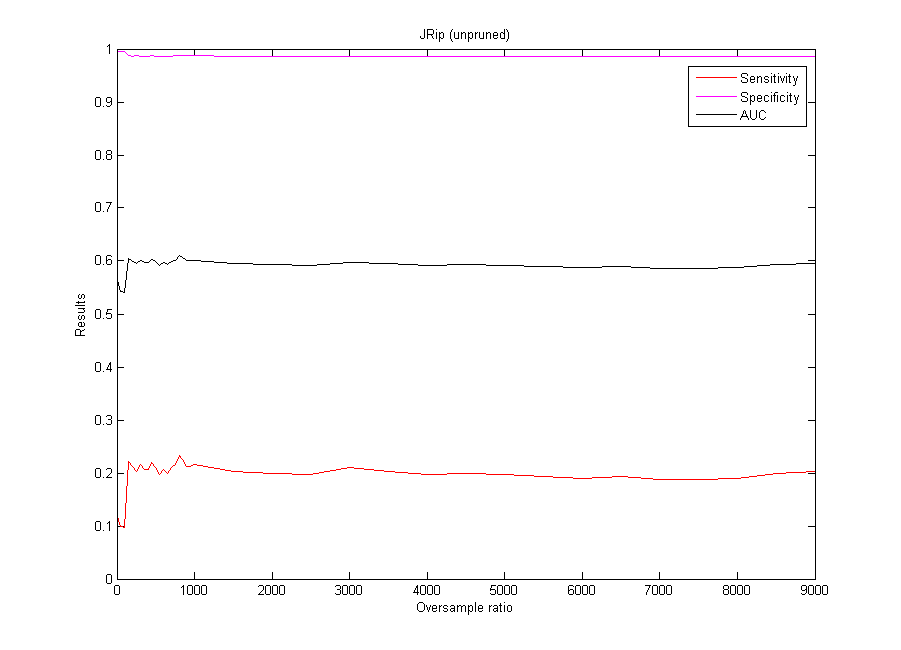
\includegraphics[scale=0.65]{img/SMOTE_JRip-unpruned.png}
\caption{\textbf{SMOTE and JRip} (unpruned decision rules) - A similar sitation as in~\ref{fig:exp-smote-j48} occurs, however a higher sensitivity is obtained. A maximum AUC of 0.6096 is achieved at a misclassification cost of 800. This classifier also yields the maximum sensitivity of 23.23\% (specificity: 98.70\%).}
\end{figure}

\newpage
\label{exp-smote-nb}
\begin{figure}[h]
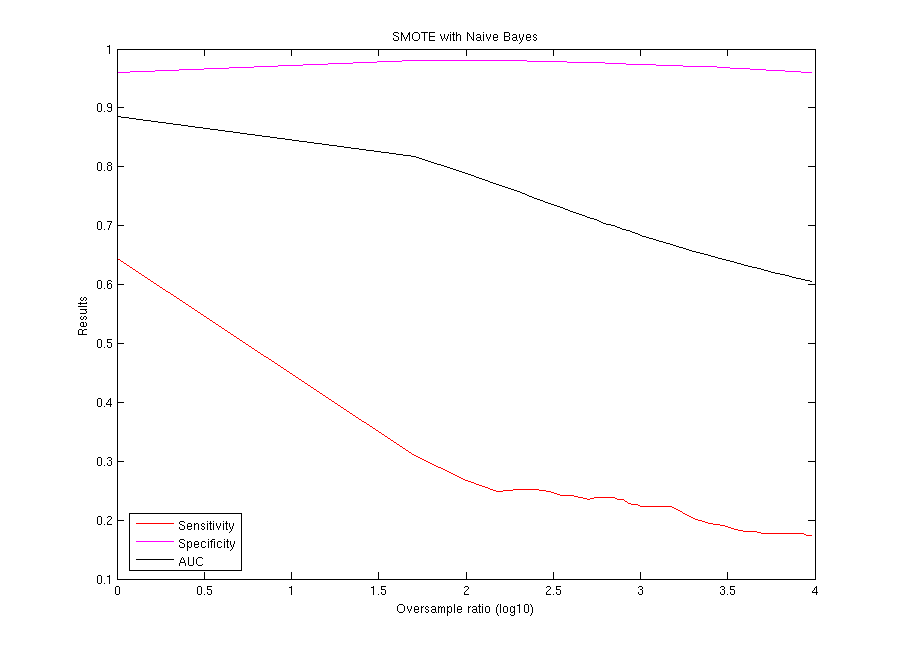
\includegraphics[scale=0.65]{img/smote.png}
\caption{\textbf{SMOTE and Naive Bayes} (Laplace smoothing) - applying SMOTE clearly worsens the performance with a Naive Bayes classifier.  A maximum AUC of 0.8851 is achieved at a  misclassification cost of 1. This classifier also yields the maximum sensitivity of 64.51\% (specificity: 95.94\%).}
\end{figure}

\newpage
\begin{figure}[h]
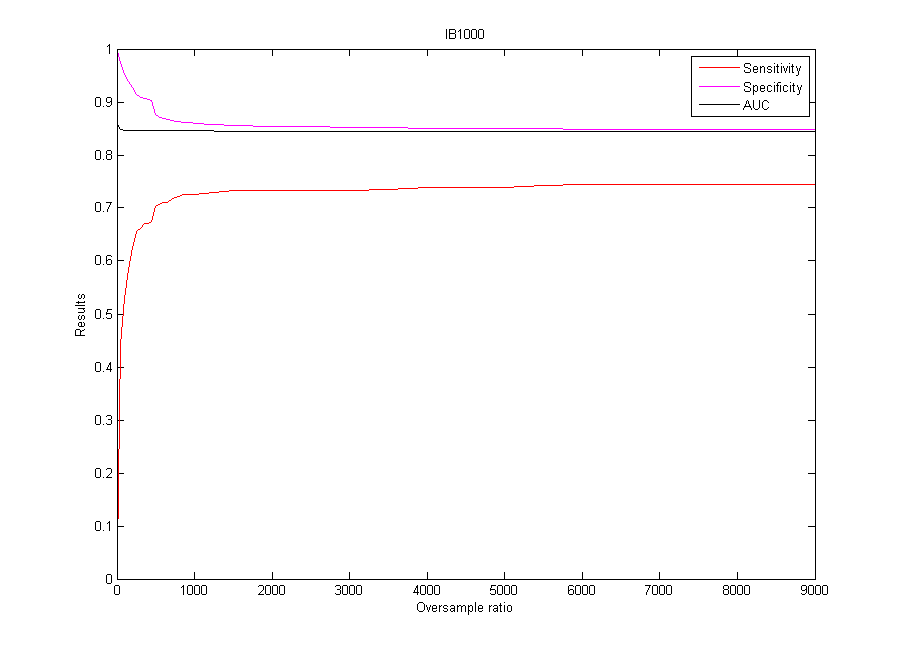
\includegraphics[scale=0.65]{img/SMOTE_IB1000.png}
\caption{\textbf{SMOTE and IBk} (1000NN) - IBk is the only classifier SMOTE seems to perform well with. A maximum AUC of 0.8616 is achieved at a  misclassification cost of 1. This classifier yields a sensitivity of 0.00\% and a specificity of 100.00\%. At a misclassification cost of 6000, a maximum sensitivity of 74.52\% is obtained (specificity: 84.88\%).}
\end{figure}

\newpage
\begin{figure}[h]
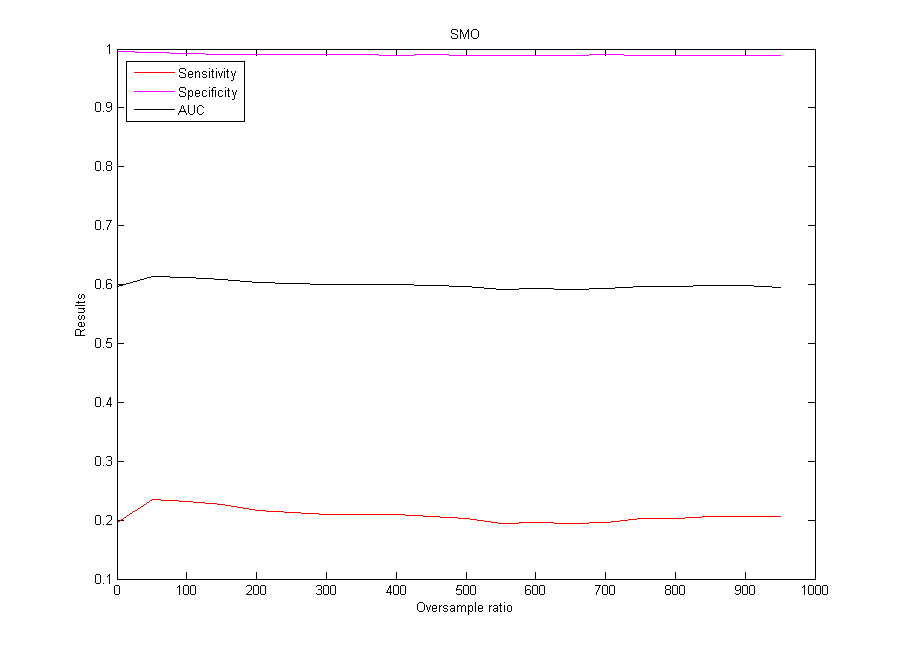
\includegraphics[scale=0.65]{img/SMOTE_SMO.png}
\caption{\textbf{SMOTE and SMO} (complexity parameter $c = 1$, linear exponent) - Experiment results of SMOTE with SMO. A maximum AUC of 0.6145 is achieved at a  misclassification cost of 50. This classifier also yields a maximum sensitivity of 23.55\% (specificity: 99.35\%).}
\end{figure}

%-------------------------------------------------------------------------------------------------------------------
% Bagging
%-------------------------------------------------------------------------------------------------------------------
\newpage
\subsection{Bagging for Imbalanced Datasets}\label{exp-bagging}
Bagging for Imbalanced Data is an extension to regular bagging which was proposed by Tao et al.~\cite{1137548}. The approach consists of generating bootstrap samples where the several classes are sampled with different ratios, hence achieving over- and/or under-sampling. In the following experiments, we create an ensemble of 10 classifiers which are trained on bootstraps where the minority class is over-sampled. In order to keep the number of experiments realistic, we only test those types of classifiers that proved most promising (highest AUC) in cost-sensitivity analysis.

\begin{figure}[h]
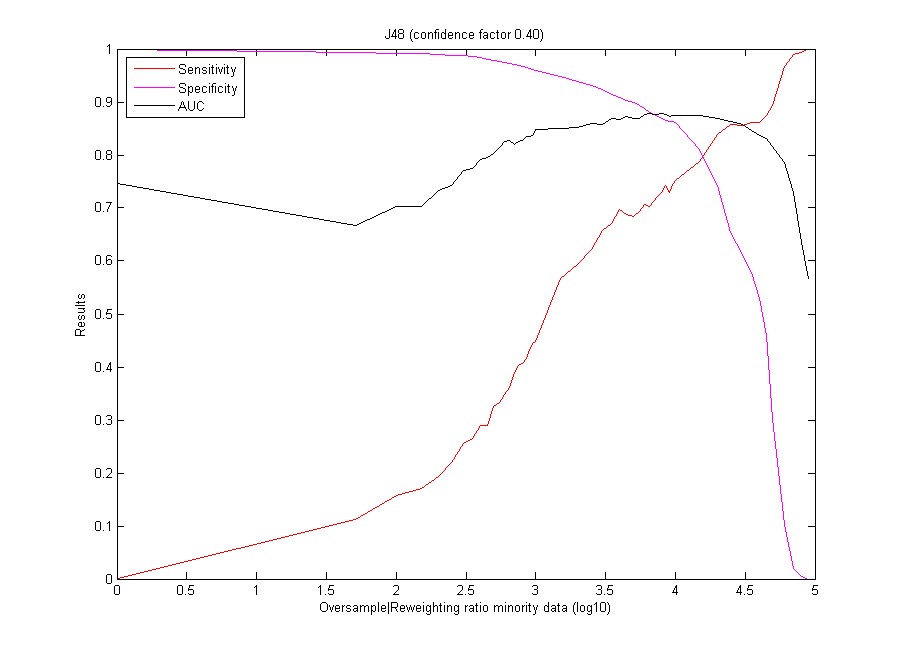
\includegraphics[scale=0.65]{img/bi_J48-confid040.png}
\caption{\textbf{Bagging with J48} (confidence factor 0.40) - Experiment results of Bagging for Imbalanced Datasets with J48. This technique allows J48 to achieve a maximum AUC of 0.8783 at a misclassification cost of 6\,500. This classifier yields a sensitivity of 70.32\% and a specificity of 88.06\%. A sensitivity of 96.77\% is achieved using a misclassification cost of 60\,000, and yields a specificity of 10.36\%. Finally, a maximum sensitivity of 100.00\% is obtained together with a specificity of 0.00\%.}
\end{figure}

\newpage
\begin{figure}[h]
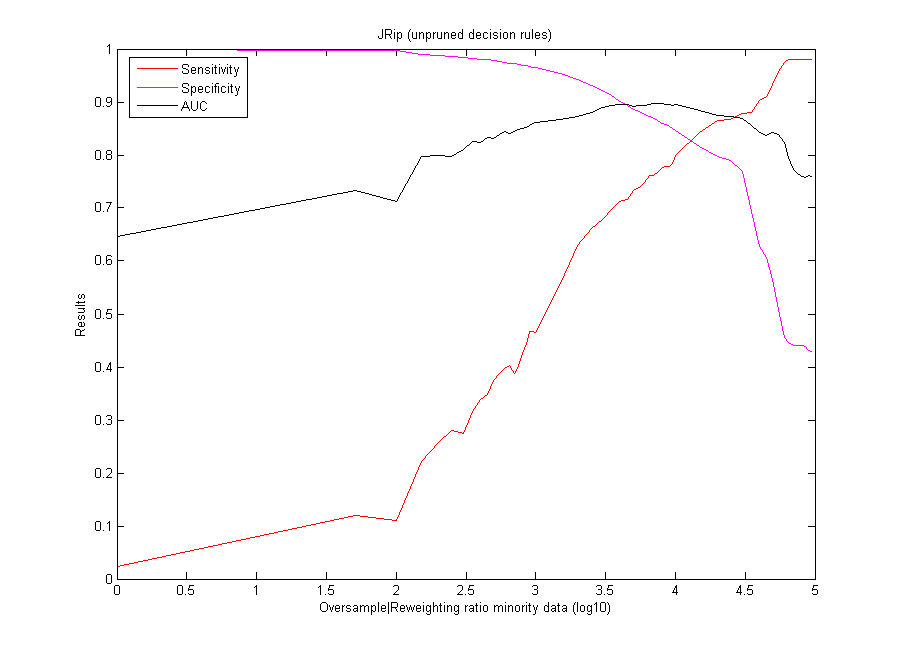
\includegraphics[scale=0.65]{img/bi_JRip-unpruned.png}
\caption{\textbf{Bagging with JRip} (unpruned decision rules) - Experiment results of Bagging for Imbalanced Datasets with JRip. This technique allows JRip to achieve a maximum AUC of 0.8976 at a misclassification cost of 7\,001. This classifier yields a sensitivity of 76.13\% and a specificity of 86.82\%. A sensitivity of 90.32\% is achieved using a misclassification cost of 40\,001, and yields a specificity of 62.80\%. Finally, a maximum sensitivity of 98.06\% is obtained together with a specificity of 44.56\%.}
\end{figure}

\newpage
\begin{figure}[h]
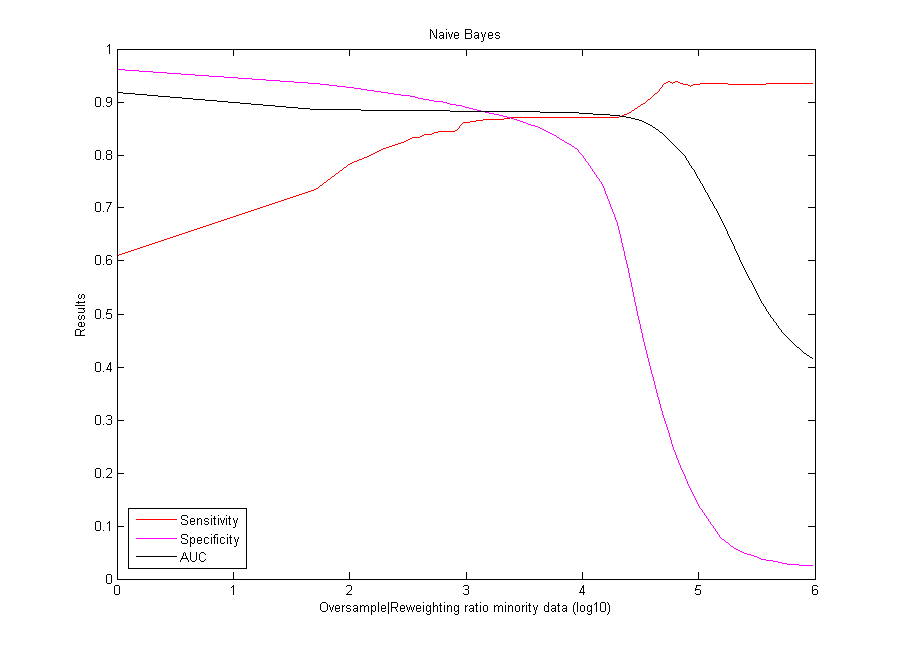
\includegraphics[scale=0.65]{img/bi_NaiveBayes.png}
\caption{\textbf{Bagging with Naive Bayes} - Experiment results of Bagging for Imbalanced Datasets with Naive Bayes. This technique allows Naive Bayes to achieve a maximum AUC of 0.9180 at a misclassification cost of 1. This classifier yields a sensitivity of 60.97\% and a specificity of 96.16\%. A sensitivity of 90.32\% is achieved using a misclassification cost of 40\,001, and yields a specificity of 62.80\%. Finally, a maximum sensitivity of 93.87\% is obtained together with a specificity of 27.76\%.}
\end{figure}

\newpage
\begin{figure}[h]
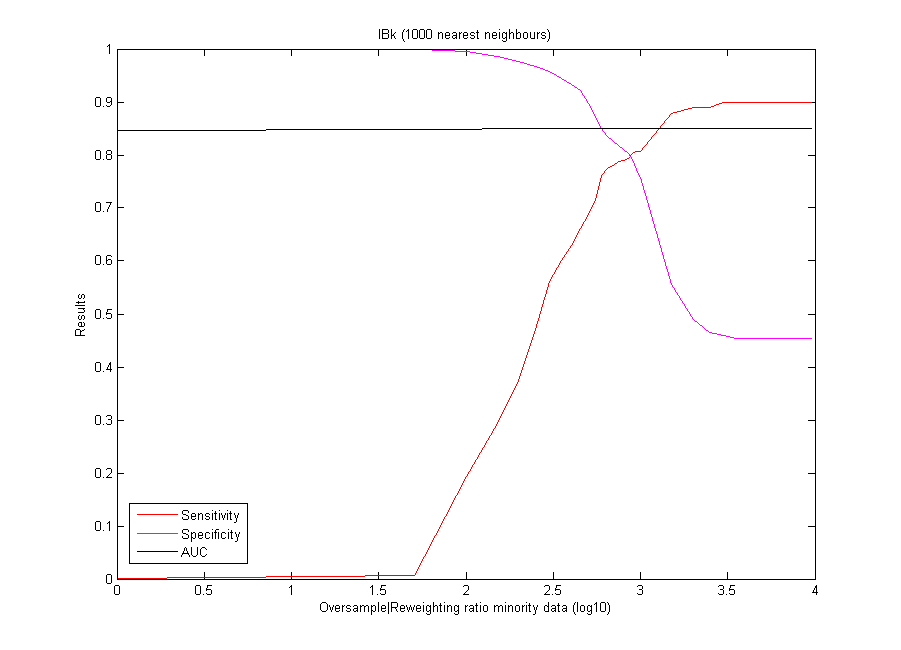
\includegraphics[scale=0.65]{img/bi_IBk-1000NN.png}
\caption{\textbf{Bagging with IBk} (1000NN) - Experiment results of Bagging for Imbalanced Datasets with IBk. This technique allows IBk to achieve a maximum AUC of 0.8507 at a misclassification cost of 9\,501. This classifier yields a sensitivity of 90.00\% and a specificity of 45.39\%. This is as well the highest obtained sensitivity.}
\end{figure}

\newpage
\begin{figure}[h]
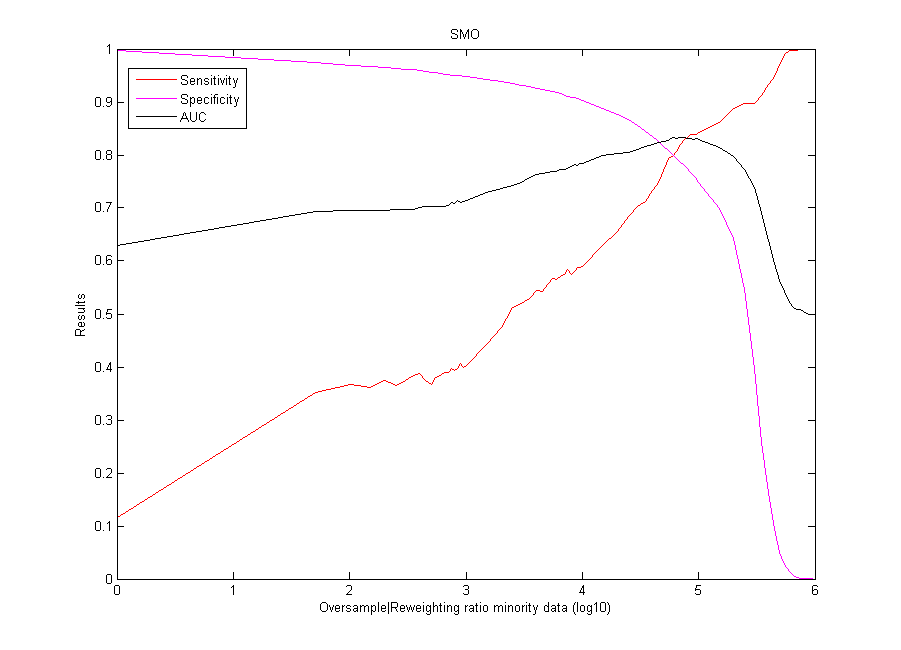
\includegraphics[scale=0.65]{img/bi_SMO.png}
\caption{\textbf{Bagging with SMO} (complexity parameter $c = 1$, linear exponent) - Experiment results of Bagging for Imbalanced Datasets with SMO. This technique allows SMO to achieve a maximum AUC of 0.8339 at a misclassification cost of 70\,001. This classifier yields a sensitivity of 81.94\% and a specificity of 78.65\%. A sensitivity of 91.29\% is achieved using a misclassification cost of 350\,001, and yields a specificity of 25.69\%. Finally, a maximum sensitivity of 100.00\% is obtained together with a specificity of 0.15\%.}
\end{figure}

\newpage
\subsection{Other Learning Techniques}\label{exp-other}

\subsubsection{REMED}
The following evaluations were performed by Prof. Luis Mena using the REMED learning algorithm. Some of the features needed to be preprocessed, as the REMED algorithm was initially developed to consider numeric or binary discrete attributes. For this reason, nominal attributes with three values \{0,1,2\} were converted such that (0= yes) is mapped to (0= present), and (1=no or 2=I don't know) is mapped to (1=absent).\\
Using a confidence level of p\textless{0.0001}, the three most statistically significant features were found to be \textit{Obs\_Different} (p=0), \textit{PE\_Something\_Wrong} (p=0) and \textit{Child\_seriously\_ill} (p=3,3307 e -16). These features are then used to generate independent classifiers:
\\ \\ \textbf{classifier 1} \\{\small \fbox{\parbox[b]{5in} {
(Obs\_different=0) =\textgreater{} serious\_without\_GE\_bronch=0 \\
=\textgreater{} serious\_without\_GE\_bronch=1}}}
\\ \\ \textbf{classifier 2} \\{\small \fbox{\parbox[b]{5in} {
(PE\_Something\_Wrong=0) =\textgreater{} serious\_without\_GE\_bronch=0 \\
=\textgreater{} serious\_without\_GE\_bronch=1}}}
\\ \\ \textbf{classifier 3} \\{\small \fbox{\parbox[b]{5in} {
(Child\_seriously\_ill=0) =\textgreater{} serious\_without\_GE\_bronch=0 \\
=\textgreater{} serious\_without\_GE\_bronch=1}}}
\\ \\ When the continuous attributes are analysed, the only attribute to be found statistically significant (confidence leel of 99\%) is the age. This allows to build two better classifiers combining both types of attributes:
\\ \\ \textbf{classifier 4} \\{\small \fbox{\parbox[b]{5in} {
(PE\_Something\_Wrong=0) and (Age\textless{}=3.32) =\textgreater{} serious\_without\_GE\_bronch=0 \\
=\textgreater{} serious\_without\_GE\_bronch=1}}}
\\ \\ \textbf{classifier 5} \\{\small \fbox{\parbox[b]{5in} {
(Child\_seriously\_ill=0) and (Age\textless{}=3.32) =\textgreater{} serious\_without\_GE\_bronch=0 \\
=\textgreater{} serious\_without\_GE\_bronch=1}}}

\newpage
The results for each classifier are showed in the following table, where the AUC was calculated with the conventional binormal method through PLOTROC.xls, available at \url{http://xray.bsd.uchicago.edu/krl/KRL_ROC/software_index.htm}


\begin{tabular}{l l l l l l l}
\cr
\hline
Classifier & Accuracy & Sensitivity & Specificity & AUC & GM & Ranker \\
\hline
1 & 96,4295 & 41,1765 & 96,8982 & 65,97 & 63,1662 & 64,57 \\
2 & 96,9998 & 55,8824 & 97,3493 & 71,18 & 73,7571 & 72,47 \\
3 & 92,3382 & 58,8235 & 92,6232 & 72,13 & 73,8134 & 72,97 \\
4 & 98,2147 & 41,1765 & 98,6997 & 65,97 & 63,7503 & 64,57 \\
5 & 96,2063 & 41,1765 & 96,6742 & 65,97 & 63,0928 & 72,47 \\
\hline
\cr
\end{tabular}

\paragraph*{Conclusion}Although REMED is developed to focus on the class imbalance problem, resulting classifiers are not satisfiable for practical purpose due to the low sensitivities. 

\newpage
\subsubsection{Thresholding Naive Bayes}
Cost-sensitivity analysis showed that the highest AUC (namely 0.9040) is obtained by a Naive Bayes classifier. For this reason, we analyse the effect of altering the class probability threshold for this classifier.
\begin{figure}[h]
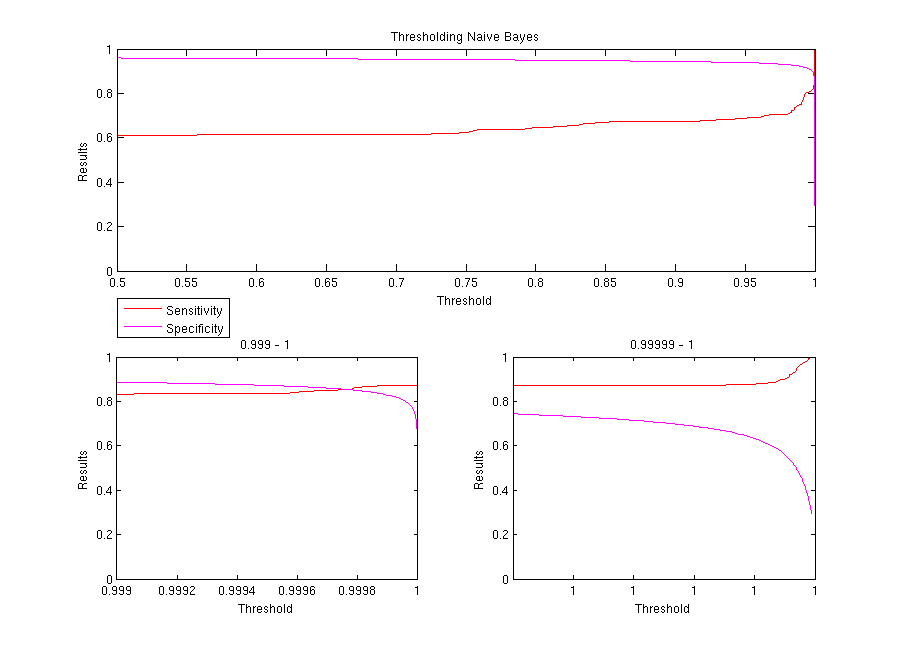
\includegraphics[scale=0.65]{img/thh_naivebayes.png}
\end{figure}

Results show that increasing the threshold can significantly affect the sensitivity. For example, when the threshold is altered from 50\% to 99.9999\%, a sensitivity of 90.3226\% and a specificity of 55.8177\%.


\newpage
\subsection{Summary}\label{exp-summary}
The following tables show an overview of the experiment results. For each experiment, the highest achieved AUC (and the the sample ratio to obtain this classifier) is displayed together with the highest obtained sensitivity (and the resulting specificity).

\begin{table}[h]
\centering  
\begin{tabular}{ l | c r | r r|}                                      
& \multicolumn{2}{c}{max AUC (sample ratio)} & \multicolumn{2}{c}{max sensitivity (specificity)} \\
\hline 
\multicolumn{5}{l}{\textbf{Cost-sensitivity}}\\
\hline
J48 (confidence factor 0.25) & 0.8536 & (13\,250) & 99.35\% & (0.67\%)\\
J48 (confidence factor 0.40) & 0.8478 & (18\,400) & 96.77\% & (6.21\%)\\
J48 (confidence factor 0.65) & 0.8431 & (19\,600) & 99.03\% & (1.32\%)\\
JRip (pruned) & 0.8431 & (466) & 99.03\% & (29.13\%)\\
JRip (unpruned) & 0.8473 & (33\,350) & 97.74\% & (43.00\%)\\
Naive Bayes (Laplace smoothing) & 0.9040 & (1) & 95.48\% & (26.95\%)\\
Naive Bayes (no smoothing) & 0.6653 & (1) & 65.16\% & (52.83\%)\\
IB3 & 0.5368 & (1) & 6.45\% & (99.59\%)\\
IB10 & 0.6044 & (1) & 20.65\% & (98.48\%)\\
IB50 & 0.7683 & (1) & 56.13\% & (95.71\%)\\
IB200 & 0.8182 & (1) & 69.68\% & (87.77\%)\\
IB1000 & 0.8539 & (601) & 90.00\% & (45.66\%)\\
IB2000 & 0.8644 & (5\,001) & 96.77\% & (1.48\%)\\
SMO & 0.8111 & (70\,250) & 84.52\% & (75.63\%)\\
CART (min 50 nodes/leaf) & - & - & 74.19\% & (91.19\%)\\
CART (min 100 nodes/leaf) & - & - & 77.42\% & (90.13\%)\\
CART (min 150 nodes/leaf) & - & - & 87.10\% & (64.67\%)\\
CART (min 200 nodes/leaf) & - & - & 80.65\% & (50.99\%)\\
\hline                          % inserts single-line
\end{tabular}
\label{tab:CostSens}
\caption{Summary of classifier performance (Cost-sensitivity)} % title name of the table
\end{table}

\paragraph{Cost-sensitivity} Results show that especially JRip and Naive Bayes (when estimates are smoothed by Laplace) are interesting classifiers when over-sampled (by means of cost-sensitivity). Decision tree classifiers such as J48 and CART on the other hand do not perform well when the minority class data is over-sampled. Although less pruning can increase the recognition of the minority class, it tends to decrease the recognition of the majority class. This observation confirms the discussion in section~\ref{causestheproblem} about the influence of class and feature noise on the recognition of outliers. A similar story happens with IBk. When the number of nearest neighbours is small (large), low recognition rates for the minority (majority) class are obtained. This observation is founded by the fact that nearest neighbours algorithms typically are sensitive to noise.

Finally, it is not clear how well SMO can perform in datasets with class imbalance. Because SMO is a very time-consuming algorithm, experiments were only performed using the most basic parameters and kernels. Hence, it is possible that the use of different kernels and/or complexity parameters can improve the performance.

\newpage
\paragraph{SMOTE} Synthetic sampling (such as SMOTE) was discussed as a another approach to sampling besides instance reweighting. Although SMOTE can decrease the risk of overfitting, experiment results are not very optimistic. In many tested classifiers, SMOTE obtains a worse performance than cost-sensitivity. Moreover, applying SMOTE with Naive Bayes learning decreases (rather than increases) the recognition rate of the minority class. The only classifier where SMOTE increases performance, is IBk. This is probably related to the fact that SMOTE performs local smoothing on the training set, which matches the inductive bias of $k$-nearest neighbours~\cite{joydeep07}. It should however be clear that the (minority) data is not always forming clusters of at least $k$ instances. When these assumptions are violated, SMOTE increases the level of noise. Given the pessimistic experiment results of SMOTE, we have reason to believe that these assumptions indeed do not hold in the KULeuven dataset.

\begin{table}[h]
\centering  
\begin{tabular}{ l | c r | r r|}                                      
& \multicolumn{2}{c}{max AUC (sample ratio)} & \multicolumn{2}{c}{max sensitivity (specificity)} \\
\hline
\multicolumn{5}{l}{\textbf{SMOTE}}\\
\hline
J48 (confidence factor 0.50) & 0.6750 & (151) & 13.87\% & (99.55\%)\\
JRip (unpruned) & 0.6096 & (801) & 23.23\% & (98.70\%)\\
Naive Bayes (Laplace smoothing) & 0.9040 & (1) & 64.52\% & (95.94\%)\\
IB1000 & 0.8616 & (1) & 74.52\% & (84.88\%)\\
SMO & 0.6145 & (51) & 23.55\% & (99.35\%)\\
\hline
\end{tabular}
\label{table:Performance02}
\caption{Summary of classifier performance (SMOTE)} % title name of the table
\end{table}

\paragraph{MetaCost} MetaCost mainly seems to have a positive effect on Naive Bayes classifiers. This is probably related to the fact that Naive Bayes learning strongly depends on the quality of the estimated prior estimates. Since MetaCost uses a bagging scheme to estimate the class probabilities, the quality of these estimates is improved. 

\begin{table}[h]
\centering  
\begin{tabular}{ l | c r | r r|}  
& \multicolumn{2}{c}{max AUC (sample ratio)} & \multicolumn{2}{c}{max sensitivity (specificity)} \\
\hline
\multicolumn{5}{l}{\textbf{MetaCost}}\\
\hline
J48 (confidence factor 0.40) & 0.7846 & (251) & 97.74\% & (0.00\%)\\
JRip (unpruned) & 0.6565 & (51) & 100.00\% & (0.00\%)\\
Naive Bayes (Laplace smoothing) & 0.9206 & (1) & 100.00\% & (12.54\%)\\
SMO & 0.6299 & (51) & 26.77\% & (99.22\%)\\
\hline
\end{tabular}
\label{table:Performance02}
\caption{Summary of classifier performance (MetaCost)} % title name of the table
\end{table}

\paragraph{Bagging for Imbalanced Datasets} Bagging for Imbalanced Datasets seems to have a positive influence on the performance of all classifiers. Because bagging reduces the variance, it helps to avoid overfitting (and therefore to increase the recognition rate of the minority class).

\begin{table}[h]
\centering  
\begin{tabular}{ l | c r | r r|}  
& \multicolumn{2}{c}{max AUC (sample ratio)} & \multicolumn{2}{c}{max sensitivity (specificity)} \\
\hline
\multicolumn{5}{l}{\textbf{Bagging for Imbalanced Datasets}}\\
\hline
J48 (confidence factor 0.40) & 0.8783 & (6500) & 100.00\% & (0.00\%)\\
JRip (unpruned) & 0.8976 & (7001) & 98.06\% & (44.56\%)\\
Naive Bayes (Laplace smoothing) & 0.9180 & (1) & 93.87\% & (27.76\%)\\
IB1000 & 0.8507 & (9501) & 90.00\% & (46.01\%)\\
SMO & 0.8339 & (70001) & 100.00\% & (0.15\%)\\
\hline
\end{tabular}
\label{table:Performance02}
\caption{Summary of classifier performance (Bagging for Imbalanced Datasets)} % title name of the table
\end{table}

\newpage
Finally, altering probability thresholds seems an interesting approach to improve classification in datasets with class imbalance, especially when applied to a Naive Bayes classifier. In general, altering the probability thresholds allows a good sensitivity-specificity tradeoff when applied to classifiers with a high AUC.

\begin{table}[h]
\centering  
\begin{tabular}{ l | c r | r r|}  
& \multicolumn{2}{c}{max AUC (sample ratio)} & \multicolumn{2}{c}{max sensitivity (specificity)} \\
\hline
\multicolumn{5}{l}{\textbf{Other}}\\
\hline
REMED & 0.7213 & - & 58.82\% & (92.62\%)\\
Naive Bayes (Thresholding) & 0.9040 & (1) & 99.68\% & (33.16\%)\\
\hline                          % inserts single-line
\end{tabular}
\label{table:Performance02}
\caption{Summary of classifier performance (Other)} % title name of the table
\end{table}



%-------------------------------------------------------------------------------------------------------------------
% RNB-FVB
%-------------------------------------------------------------------------------------------------------------------
\newpage
\section{Experiment results of Naive Bayes Sampling}\label{exp-rnb}
In this section, we investigate the performance of Naive Bayes Sampling by applying different sampling ratios, as introduced in chapter~\ref{newapproach}. The number of Naive Bayes classifiers in each ensemble is restricted to 10. 
We evaluate the classifiers by applying stratified 10-fold cross-validation (which is repeated over 10 randomized runs), and measure the AUC, sensitivity and specificity. Afterwards, we compare these results to the ones obtained by combining Naive Bayes learning with Cost-Sensitivity (see section~\ref{cost-sensitivity}), MetaCost and Bagging for Imbalanced Datasets (see section~\ref{classif-ensembles}).

\newpage
\subsection{Ill Children (KULeuven)}
\begin{figure}[h]
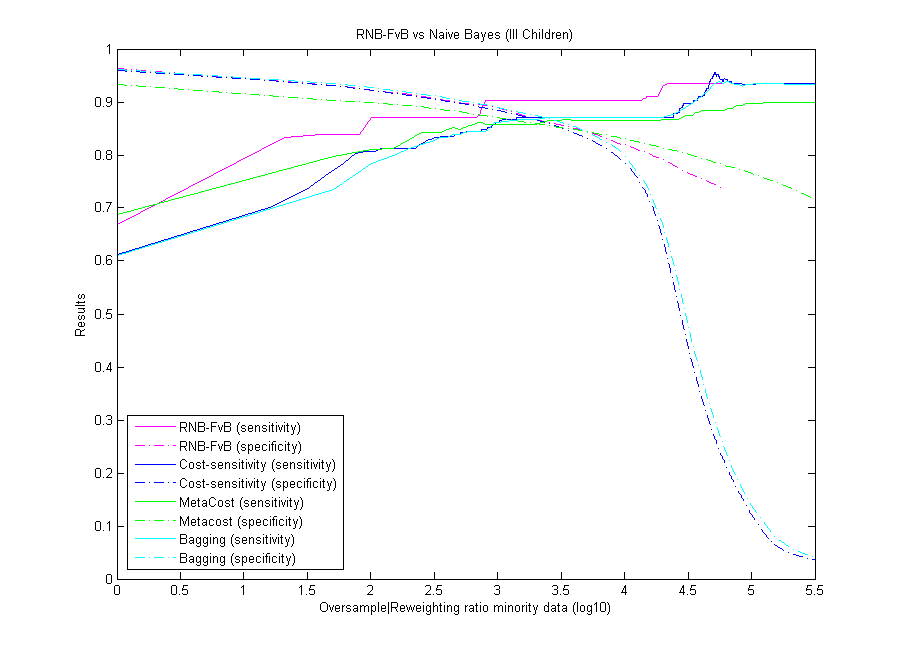
\includegraphics[scale=0.65]{img/RNB-FvB-illchildren.png}
\caption{Experiment results of Naive Bayes Sampling on \textbf{Ill Children}}
\end{figure}
 
\begin{table}[h]
\centering  
\begin{tabular}{ l | c r | r r|}                                      
& \multicolumn{2}{c}{max AUC (sample ratio)} & \multicolumn{2}{c}{max sensitivity (specificity)} \\
\hline 
Naive Bayes Sampling & 0.9479 & (x\,60\,000) & 93.55\% & (78.61\%)\\
Cost-sensitivity & 0.9040 & (x\,1) & 95.48\% & (26.95\%)\\
MetaCost & 0.9206 & (x\,1) & 100.00\% & (12.54\%)\\
Bagging & 0.9190 & (x\,1) & 93.87\% & (27.76\%)\\
\hline                          % inserts single-line
\end{tabular}
\label{tab:PPer}
\caption{Overview Results Naive Bayes Sampling for Ill Children} % title name of the table
\end{table}
 

\newpage
\subsection{Breast-Cancer (UCI)}
\begin{figure}[h]
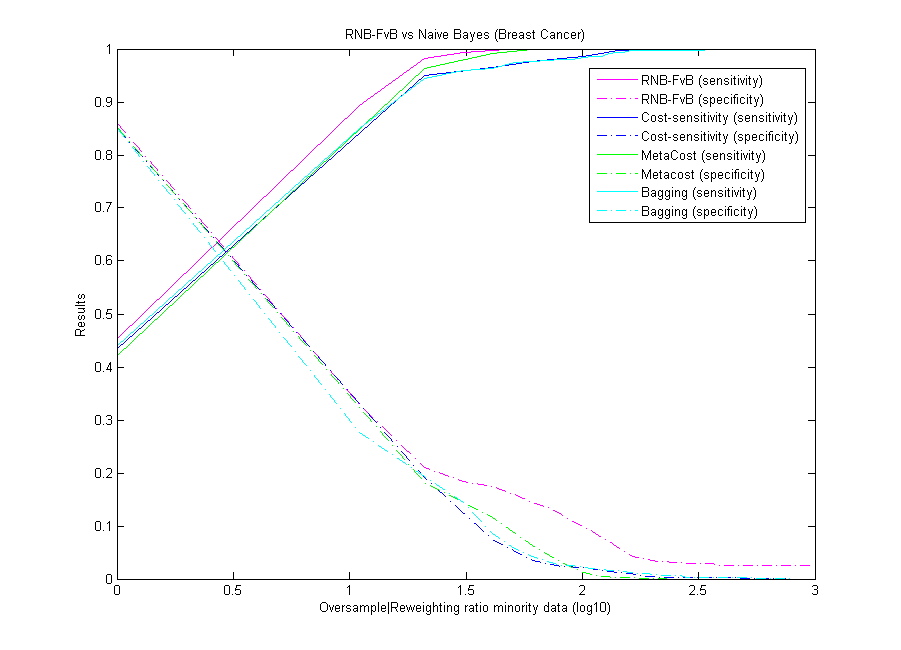
\includegraphics[scale=0.65]{img/RNB-FvB-breastcancer.png}
\caption{Experiment results of Naive Bayes Sampling on \textbf{Breast Cancer}}
\end{figure}

\begin{table}[h]
\centering  
\begin{tabular}{ l | c r | r r|}                                      
& \multicolumn{2}{c}{max AUC (sample ratio)} & \multicolumn{2}{c}{max sensitivity (specificity)} \\
\hline 
Naive Bayes Sampling & 0.7450 & (x\,271) & 100.00\% & (15.92\%)\\
Cost-sensitivity & 0.6981 & (x\,1) & 100.00\% & (0.30\%)\\
MetaCost & 0.7187 & (x\,41) & 100.00\% & (3.03\%)\\
Bagging & 0.6995 & (x\,1) & 100.00\% & (0.00\%)\\
\hline                          % inserts single-line
\end{tabular}
\label{tab:PPer}
\caption{Overview Results Naive Bayes Sampling for Breast Cancer} % title name of the table
\end{table}


\newpage
\subsection{Hepatitis (UCI)}
\begin{figure}[h]
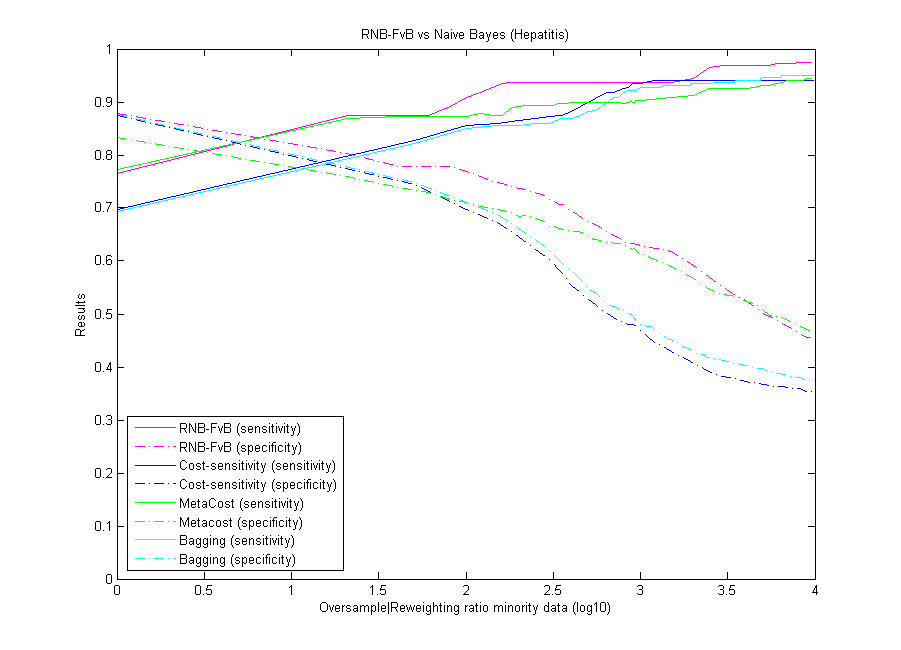
\includegraphics[scale=0.65]{img/RNB-FvB-hepatitis.png}
\caption{Experiment results of Naive Bayes Sampling on \textbf{Hepatitis}}
\end{figure}

\begin{table}[h]
\centering  
\begin{tabular}{ l | c r | r r|}                                      
& \multicolumn{2}{c}{max AUC (sample ratio)} & \multicolumn{2}{c}{max sensitivity (specificity)} \\
\hline 
Naive Bayes Sampling & 0.9101 & (x\,7\,500) & 97.50\% & (46.42\%)\\
Cost-sensitivity & 0.8639 & (x\,51) & 94.06\% & (44.72\%)\\
MetaCost & 0.8710 & (x\,21) & 94.37\% & (47.07\%)\\
Bagging & 0.8746 & (x\,51) & 95.00\% & (38.86\%)\\
\hline                          % inserts single-line
\end{tabular}
\label{tab:PPer}
\caption{Overview Results Naive Bayes Sampling for Hepatitis} % title name of the table
\end{table}

\newpage
\subsection{Sick (UCI)}
\begin{figure}[h]
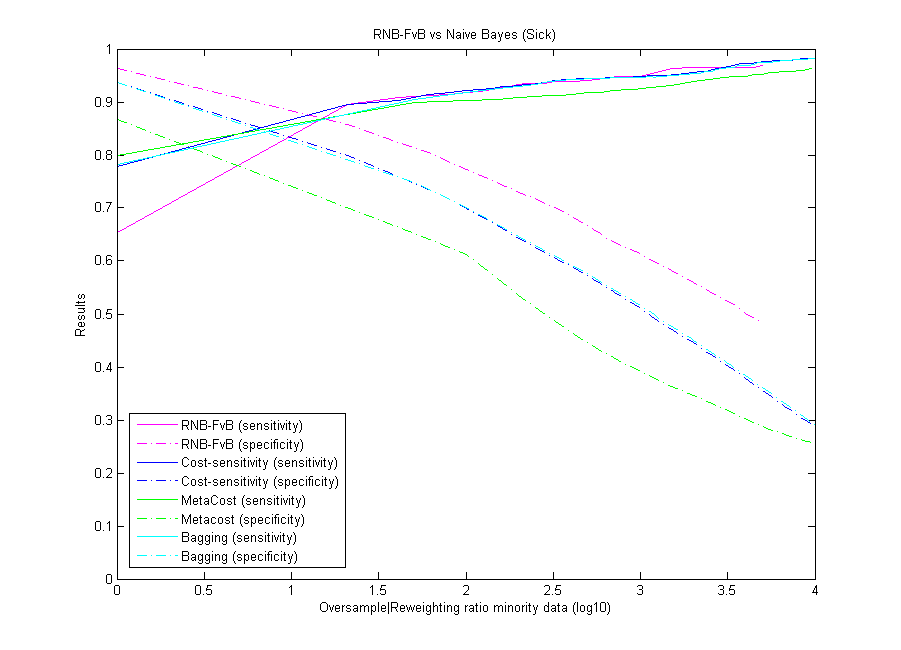
\includegraphics[scale=0.65]{img/RNB-FvB-sick.png}
\caption{Experiment results of Naive Bayes Sampling on \textbf{Sick}}
\end{figure}

\begin{table}[h]
\centering  
\begin{tabular}{ l | c r | r r|}                                      
& \multicolumn{2}{c}{max AUC (sample ratio)} & \multicolumn{2}{c}{max sensitivity (specificity)} \\
\hline 
Naive Bayes Sampling & 0.9322 & (x\,1) & 96.97\% & (48.18\%)\\
Cost-sensitivity & 0.9253 & (x\,1) & 98.23\% & (29.74\%)\\
MetaCost & 0.8898 & (x\,1) & 96.23\% & (25.73\%)\\
Bagging & 0.9269 & (x\,1) & 98.18\% & (29.32\%)\\
\hline                          % inserts single-line
\end{tabular}
\label{tab:PPer}
\caption{Overview Results Naive Bayes Sampling for Sick} % title name of the table
\end{table}

\newpage
\subsection{Liver disorders (UCI)}
\begin{figure}[h]
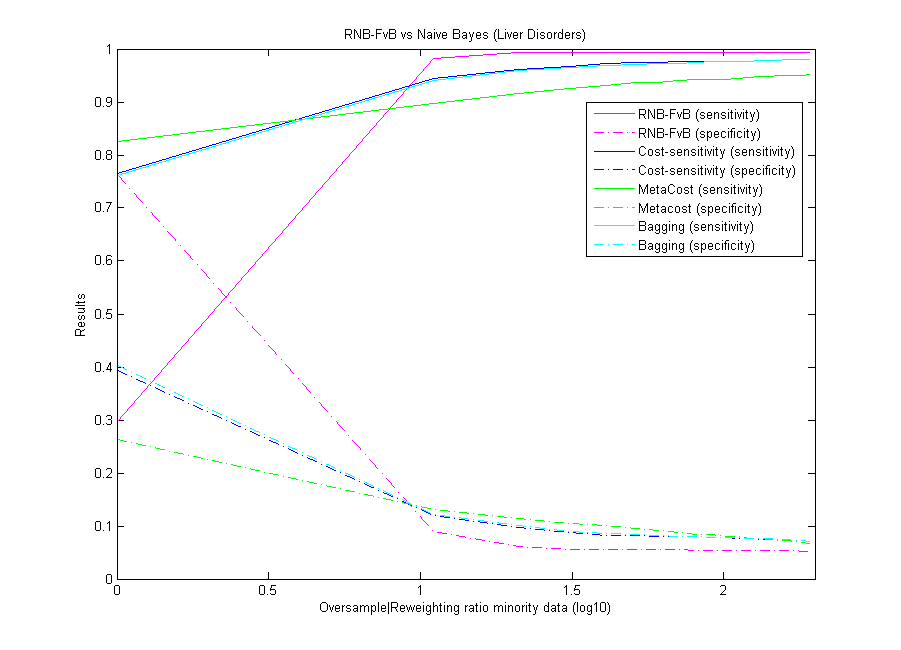
\includegraphics[scale=0.65]{img/RNB-FvB-liverdisorder.png}
\caption{Experiment results of Naive Bayes Sampling on \textbf{Liver Disorders}}
\end{figure}

\begin{table}[h]
\centering  
\begin{tabular}{ l | c r | r r|}                                      
& \multicolumn{2}{c}{max AUC (sample ratio)} & \multicolumn{2}{c}{max sensitivity (specificity)} \\
\hline 
Naive Bayes Sampling & 0.5744 & (x\,11) & 99.31\% & (6.05\%)\\
Cost-senstivity & 0.6331 & (x\,171) & 97.93\% & (7.25\%)\\
MetaCost & 0.5804 & (x\,11) & 95.10\% & (6.75\%)\\
Bagging & 0.6289 & (x\,161) & 97.93\% & (7.40\%)\\
\hline                 
\end{tabular}
\label{tab:PPer}
\caption{Overview Results Naive Bayes Sampling for Liver Disorders} 
\end{table}






%

\newpage
\section{Experiments}
Following tests performed by applying 10-fold cross-validation, averaged over 10 different randomized runs. Moreover, in order to decrease computational requirements, the number of Naive Bayes classifiers in the bagging ensemble is restricted to 10. In each experiment, results of the new approach are compared with cost-sensitivity (see~\ref{costsensitive}), MetaCost (see~\ref{MetaCost}) and Bagging for Imbalanced datasets (see~\ref{BaggingImbalanced}).

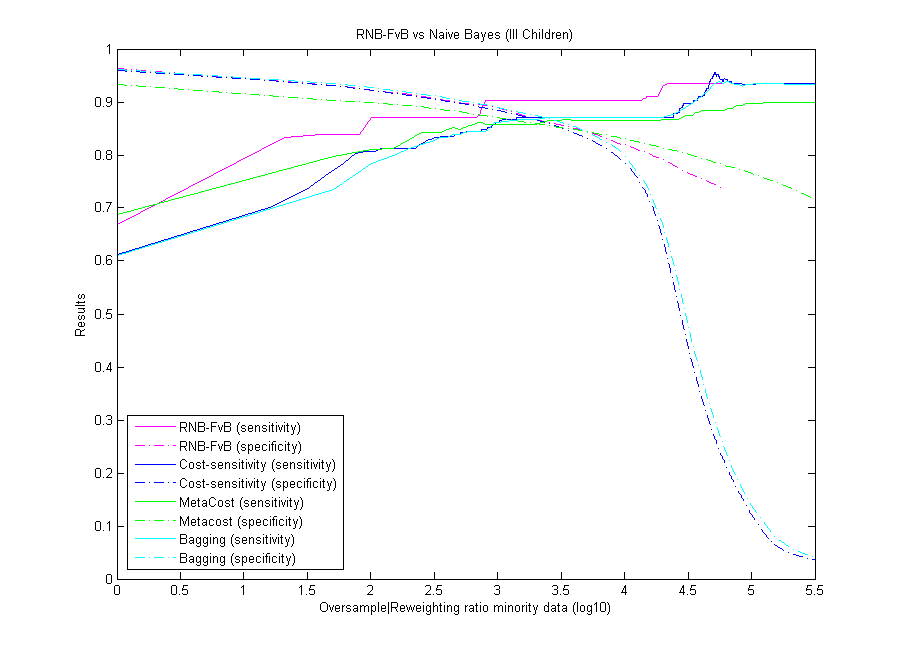
\includegraphics[scale=0.65]{img/RNB-FvB-illchildren.png}
 
\begin{table}[h]
\centering  
\begin{tabular}{ l | c r | r r|}                                      
& \multicolumn{2}{c}{max AUC (sample ratio)} & \multicolumn{2}{c}{max sensitivity (specificity)} \\
\hline 
RNB-FvB & 0.9479 & (x\,60\,000) & 93.55\% & (78.61\%)\\
Cost-sensitivity & 0.9040 & (x\,1) & 95.48\% & (26.95\%)\\
MetaCost & 0.9206 & (x\,1) & 100.00\% & (12.54\%)\\
Bagging & 0.9128 & (x\,1) & 86.45\% & (87.05\%)\\
\hline                          % inserts single-line
\end{tabular}
\label{tab:PPer}
\caption{Overview Results RNB-FvB for Ill Children} % title name of the table
\end{table}
 




\newpage
Since it is important to measure the performance of a new technique in many datasets in order to allow generalisation of results, the same tests were performed on some UCI datasets (\url{http://archive.ics.uci.edu/ml/}) and averaged over 10 randomized runs:\\\\
\textbf{Breast-cancer}: the breast cancer domain was obtained from the University Medical Centre, Institute of Oncology, Ljubljana, Yugoslavia (1988). Thanks go to M. Zwitter and M. Soklic for providing the data. The data set includes 85 instances of one class (\textit{recurrence-events}) and 201 instances of another class (\textit{no-recurrence-events}). The instances are described by 9 attributes, of which all are nominal. In the following graph, performance results of Random Naive Bayes with Feature-value bootstrapping is compared with regular Naive Bayes (reweighting the \textit{recurrence-events} class).

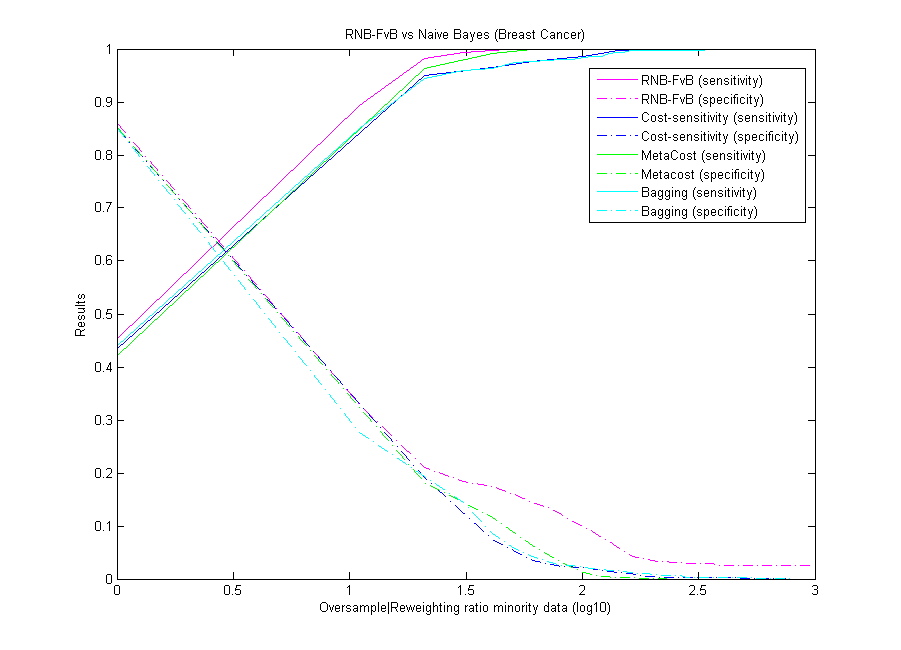
\includegraphics[scale=0.65]{img/RNB-FvB-breastcancer.png}

\begin{table}[h]
\centering  
\begin{tabular}{ l | c r | r r|}                                      
& \multicolumn{2}{c}{max AUC (sample ratio)} & \multicolumn{2}{c}{max sensitivity (specificity)} \\
\hline 
RNB-FvB & 0.7450 & (x\,271) & 100.00\% & (15.92\%)\\
Cost-sensitivity & 0.6981 & (x\,1) & 100.00\% & (0.30\%)\\
MetaCost & 0.7187 & (x\,41) & 100.00\% & (3.03\%)\\
Bagging & 0.6951 & (x\,1) & 95.65\% & (15.87\%)\\
\hline                          % inserts single-line
\end{tabular}
\label{tab:PPer}
\caption{Overview Results RNB-FvB for Breast-cancer} % title name of the table
\end{table}


\newpage
\textbf{Hepatitis}: the hepatitis domain was donated by G. Gong, Carnegie-Mellon University, Ljubljana, Yugoslavia (1988). The data set includes 32 instances of one class (\textit{die}) and 123 instances of another class (\textit{live}). The instances are described by 19 attributes, of which 6 are numeric and 13 are nominal. In the following graph, performance results of Random Naive Bayes with Feature-value bootstrapping is compared with regular Naive Bayes (reweighting the \textit{die} class).
 
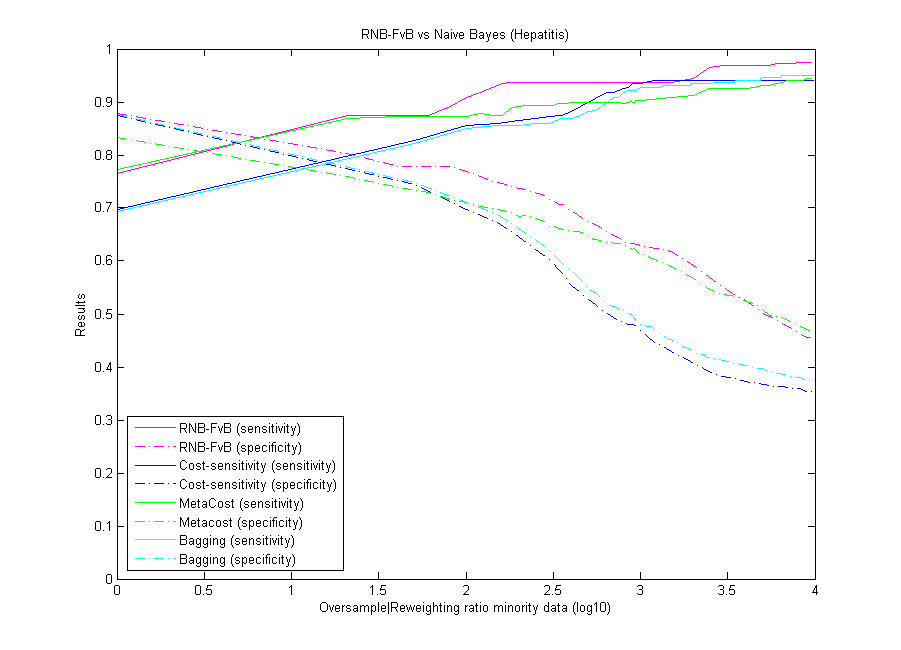
\includegraphics[scale=0.65]{img/RNB-FvB-hepatitis.png}

\begin{table}[h]
\centering  
\begin{tabular}{ l | c r | r r|}                                      
& \multicolumn{2}{c}{max AUC (sample ratio)} & \multicolumn{2}{c}{max sensitivity (specificity)} \\
\hline 
RNB-FvB & 0.9101 & (x\,7\,500) & 97.50\% & (46.42\%)\\
Cost-sensitivity & 0.8639 & (x\,51) & 94.06\% & (44.72\%)\\
MetaCost & 0.8710 & (x\,21) & 94.37\% & (47.07\%)\\
Bagging & 0.8723 & (x\,1) & 95.31\% & (44.39\%)\\
\hline                          % inserts single-line
\end{tabular}
\label{tab:PPer}
\caption{Overview Results RNB-FvB for Hepatitis} % title name of the table
\end{table}

\newpage
\textbf{Sick}: this dataset conciders Thyroid disease records supplied by the Garavan Institute and the New South Wales Institute (J. Ross Quinlan), Sydney, Australia. The dataset includes 231 instances of one class (\textit{sick}) and 3541 instances of another class (\textit{negative}). The instances are described by 29 attributes, of which  7 are continuous and 23 are discrete. In the following graph, performance results of Random Naive Bayes with Feature-value bootstrapping is compared with regular Naive Bayes (reweighting the \textit{sick} class).

\includegraphics[scale=0.65]{img/RNB-FvB-sick.png}

\begin{table}[h]
\centering  
\begin{tabular}{ l | c r | r r|}                                      
& \multicolumn{2}{c}{max AUC (sample ratio)} & \multicolumn{2}{c}{max sensitivity (specificity)} \\
\hline 
RNB-FvB & 0.9322 & (x\,1) & 96.97\% & (48.18\%)\\
Cost-sensitivity & 0.9253 & (x\,1) & 98.23\% & (29.74\%)\\
MetaCost & 0.8898 & (x\,1) & 96.23\% & (25.73\%)\\
Bagging & 0.9281 & (x\,1) & 96.84\% & (36.92\%)\\
\hline                          % inserts single-line
\end{tabular}
\label{tab:PPer}
\caption{Overview Results RNB-FvB for Sick} % title name of the table
\end{table}

\newpage
\textbf{Liver-disorders}: This dataset contains blood tests (taken from male individuals) which are thought to be sensitive to liver disorders that might arise from excessive alcohol consumption. The dataset includes 145 instances of one class and 200 instances of another class. The instances are described by 6 attributes, of which all are continuous. In the following graph, performance results of Random Naive Bayes with Feature-value bootstrapping is compared with regular Naive Bayes where the minority data is reweighted.

\includegraphics[scale=0.65]{img/RNB-FvB-liverdisorder.png}

\begin{table}[h]
\centering  
\begin{tabular}{ l | c r | r r|}                                      
& \multicolumn{2}{c}{max AUC (sample ratio)} & \multicolumn{2}{c}{max sensitivity (specificity)} \\
\hline 
RNB-FvB & 0.5744 & (x\,11) & 99.31\% & (6.05\%)\\
Cost-senstivity & 0.6331 & (x\,171) & 97.93\% & (7.25\%)\\
MetaCost & 0.5804 & (x\,11) & 95.10\% & (6.75\%)\\
Bagging & 0.6328 & (x\,161) & 98.00\% & (6.65\%)\\
\hline                 
\end{tabular}
\label{tab:PPer}
\caption{Overview Results RNB-FvB for Liver-disorders} 
\end{table}
Note that the lower AUC values for RNB-FvB are probably related to the fact that the used bootstrapping technique for continuous features is a mathematically not optimal solution. However, it is clear that RNB-FvB outperforms Naive Bayes even when all features are bootstrapped this way.

\chapter{Conclusion}\label{Conclusion}
In this chapter we present our answers to the research questions and recommendations for future research. The answers are provided in section~\ref{conclusion-answer}. The recommendations are summarized in section~\ref{conclusion-recommendations}.

\section{Thesis Conclusion}\label{conclusion-answer}

Given the overview provided in chapter~\ref{imbalanced} and the experiments we showed in chapter~\ref{Experiments}, we are in position to answer our first research question:

\begin{quote}\emph{Which existing techniques improve classification in the presence of class imbalanced data?}\end{quote}

The answer to this question can be formulated as follows. The most promising techniques are based on combining ensembles and sampling techniques, which is illustrated by the experiments with Bagging for Imbalanced Datasets (section~\ref{exp-bagging}) and MetaCost (section~\ref{exp-metacost}). The results can also be improved by better estimating data distribution (e.g. Laplace estimate in a Naive Bayes classifier) or proper tuning the probability decision thresholds of scoring classifiers. In this context, we note the importance of appropriate evaluation metrics as AUC when measuring the classifier's performance.

After this answer, we continue with the second research question:

\begin{quote}\emph{Can Naive Bayes Sampling additionally improve classification for class imbalanced data?}\end{quote}

An answer to this question can mainly be found in chapter~\ref{newapproach}. Although we showed that Naive Bayes Sampling changes the bias and variance of the estimate, it is unclear what the exact relation is. The reason is that measuring the impact of imposing feature independence is a very complicated task. Similar problems moreover occur  in different approaches that implement a strategy to make the independence assumption more true. Hence, we suggest to compare different sampling schemes beside Naive Bayes Sampling before making a statement about its performance. However, experiment results show that Naive Bayes Sampling can indeed improve classification for class imbalanced data.


\section{Future Research}\label{conclusion-recommendations}
Future research will focus on the following issues. First, we will improve bootstrapping of numerical features (1) by applying exactly the same sampling scheme as for nominal feature values, or (2) by estimating different distributions than the (augmented) Gaussian. Second, we will experiment under-sampling of the majority class in very large datasets by applying Naive Bayes Sampling. Third, we will investigate a technique that penalizes existing feature dependencies depending on the amount of examples that describe them. As a result, it would be possible to present generated samples to different learning algorithms than Naive Bayes. However, given the fact that minority classes often lack in descriptive data, we are not sure if this approach would allow big improvements.


%\newpage
%\lstset{language=Java, caption=Bootstrap Filter, label=DescriptiveLabel}
\begin{lstlisting}
import java.util.*;
import weka.core.*;
import weka.core.Capabilities.*;
import weka.filters.*;


/**
 * This filter makes a bootstrap of a specific class. In order to apply it
 * correctly, the filter should be used in combination with a
 * FilteredClassifier, such that the bootstrap only uses training data
 *
 * Apr 10, 2009
 * @author Thomas Debray
 * @version $Revision: 1.0 $
 */
public class Bootstrap extends Filter implements SupervisedFilter,
        OptionHandler, TechnicalInformationHandler {

    /** the class to oversample **/
    protected int m_ClassValueIndex = 0;

     /** the seed **/
     protected int m_RandomSeed = 1;

     /** the ratio to oversample **/
     protected double m_SampleRatio = 1;


     @Override
     public Capabilities getCapabilities() {
         Capabilities result = super.getCapabilities();

         // attributes
         result.enableAllAttributes();
         result.enable(Capability.MISSING_VALUES);

         // class
         result.enable(Capability.NOMINAL_CLASS);
         result.enable(Capability.MISSING_CLASS_VALUES);
         return result;
    }
    
    

     @Override
     public boolean setInputFormat(Instances instanceInfo) throws Exception {
         super.setInputFormat(instanceInfo);
         super.setOutputFormat(instanceInfo);
         return true;
     }

    @Override
    public boolean input(Instance instance) {
        if (getInputFormat() == null)
            throw new IllegalStateException("No input instance format defined");
        if (m_NewBatch) {
            resetQueue();
            m_NewBatch = false;
        }
        if (m_FirstBatchDone) {
            push(instance);
            return true;
        } else {
            bufferInput(instance);
            return false;
        }
    }

    @Override
    public boolean batchFinished() throws Exception {
        if (getInputFormat() == null)
            throw new IllegalStateException("No input instance format defined");

        if (!m_FirstBatchDone) {
            doBootstrapping();
        }
        flushInput();

        m_NewBatch = true;
        m_FirstBatchDone = true;
        return (numPendingOutput() != 0);
    }

    private void doBootstrapping() {
        int numpos = getInputFormat().attributeStats(getInputFormat()
                .classIndex()).nominalCounts[m_ClassValueIndex];
        int [] posInd = new int[numpos];
        int [] posWeights = new int[numpos];


        //store the index of positive instances
        int k=0;
        for(int i=0; i<getInputFormat().numInstances(); i++) {
            Instance instance = (Instance) getInputFormat().instance(i);
            if (instance.classValue() == m_ClassValueIndex)
                posInd[k++] = i;
            else
                push((Instance)instance.copy());
        }

        //create n new instances
        int instancesToCreate = (int)Math.round(numpos*m_SampleRatio);
        Random random = new Random(m_RandomSeed);
        for (int i=0; i<instancesToCreate; i++)
        {
            int index = random.nextInt(numpos);
            posWeights[index]++;
        }

        //alter the weight of the instances and push them
        for (int i=0; i<numpos; i++)
        {
            Instance next = getInputFormat().instance(posInd[i]);
            next.setWeight(posWeights[i]);
            push(next);
        }
    }

    public String getRevision() {
        throw new UnsupportedOperationException("Not supported yet.");
    }

    public Enumeration listOptions() {
        Vector newVector = new Vector();
        newVector.addElement(new Option(
                "\tSpecifies the random number seed\n"
                + "\t(default 1)",
                "S", 1, "-S <num>"));
        newVector.addElement(new Option(
                "\tSpecifies the ratio to bootstrap"
                +"(default 1 - keep original\n"
                +"\tamount of positive instances)\n"
                +"\t(default 0: no oversampling))\n",
                "R", 1, "-R <value-index>"));
        newVector.addElement(new Option(
                "\tSpecifies the positive class value (default 0))\n",
                "C", 1, "-C <value-index>"));
        return newVector.elements();
    }

    public void setOptions(String[] arg0) throws Exception {
        String seedStr = Utils.getOption('S', arg0);
        if (seedStr.length() != 0) {
            setRandomSeed(Integer.parseInt(seedStr));
        } else {
            setRandomSeed(1);
        }
        String classValueIndexStr = Utils.getOption( 'C', arg0);
        if (classValueIndexStr.length() != 0)
            setClassValue(Integer.parseInt(classValueIndexStr));
        String sampleRatio = Utils.getOption('R',arg0);
        if (sampleRatio.length() != 0)
            setSampleRatio(Double.parseDouble(sampleRatio));
    }

    public String[] getOptions() {
        Vector<String>	result;

        result = new Vector<String>();
        result.add("-C");
        result.add("" + getClassValue());
        result.add("-S");
        result.add("" + getRandomSeed());
        result.add("-R");
        result.add("" + getSampleRatio());

        return result.toArray(new String[result.size()]);
    }

    public TechnicalInformation getTechnicalInformation() {
        throw new UnsupportedOperationException("Not supported yet.");
    }

    /* PARAMETER RANDOM SEED **/
    public String randomSeedTipText() {
        return "The seed used for bootstrapping.";
    }
    public int getRandomSeed() {
        return m_RandomSeed;
    }
    public void setRandomSeed(int value) {
        m_RandomSeed = value;
    }


    /* PARAMETER MINORITY CLASS VALUE **/
    public String classValueTipText() {
        return "The index of the class value which should be oversampled. ";
    }
    public void setClassValue(int value) {
        m_ClassValueIndex = value;
    }
    public int getClassValue() {
        return m_ClassValueIndex;
    }

    /* PARAMETER SAMPLE RATIO **/
    public String sampleRatioTipText() {
        return "The sample ratio of the class to be bootstrapped";
    }
    public void setSampleRatio(double value) {
        this.m_SampleRatio = value;
    }
    public double getSampleRatio() {
        return m_SampleRatio;
    }
}
\end{lstlisting}

\newpage
\bibliographystyle{acm}
\bibliography{myrefs}

\backcover
\end{document}
